\documentclass{report}
\usepackage{graphicx}
\usepackage{amsmath}
\usepackage{amsfonts}
\usepackage{amssymb}
\usepackage[utf8]{inputenc}   % see note below
\usepackage[spanish, english]{babel}
\usepackage{blindtext}
\usepackage{textcomp}
\usepackage{pgfplots}
\pgfplotsset{width=10cm,compat=1.9}
\usepackage[margin=1in]{geometry}

\pgfplotsset{compat=1.17}
\usetikzlibrary{shapes.geometric, calc}
\usepackage{caption}
\usepackage{svg,scalerel}
\usepackage{float}
\usepackage[round,authoryear]{natbib}
% Load hyperref after natbib
\usepackage[hidelinks]{hyperref}
\usepackage{hyperref}
\usepackage[hang,flushmargin]{footmisc}
\usepackage[most]{tcolorbox}
\usepackage{tikz}

\usepackage{booktabs}
\usepackage{tabularx}
\usepackage{multirow}
\usepackage{xcolor}
\usepackage{colortbl}
\usepackage[table,xcdraw]{xcolor}

%%--- 
% \usepackage{tikz}
% \usetikzlibrary{positioning,arrows.meta,calc}
% \usepackage{pdflscape}
% \usepackage{adjustbox}
% \usepackage{forest}
% \usepackage{pdflscape}

% % PREAMBLE
% \usepackage{tikz}
% \usetikzlibrary{positioning,arrows.meta}
% \usepackage{pdflscape}

\usepackage{tikz}
\usetikzlibrary{positioning,arrows.meta}

\definecolor{softblue}{RGB}{232,240,248}
\definecolor{softgreen}{RGB}{234,244,236}
\definecolor{softpeach}{RGB}{250,239,228}
\definecolor{softgrey}{RGB}{238,238,238}
\tikzset{
    root/.style={
        draw,
        rounded corners=3pt,
        fill=softgrey,
        font=\bfseries,
        align=center,
        text width=5.0cm,
        minimum height=0.9cm
    },
    bluebranch/.style={
        draw,
        rounded corners=3pt,
        fill=softblue,
        font=\bfseries,
        align=center,
        text width=3.4cm,
        minimum height=0.8cm
    },
    greenbranch/.style={
        draw,
        rounded corners=3pt,
        fill=softgreen,
        font=\bfseries,
        align=center,
        text width=3.4cm,
        minimum height=0.8cm
    },
    peachbranch/.style={
        draw,
        rounded corners=3pt,
        fill=softpeach,
        font=\bfseries,
        align=center,
        text width=3.4cm,
        minimum height=0.8cm
    },
    bluemethod/.style={
        draw,
        rounded corners=2pt,
        fill=softblue!55,
        align=center,
        font=\small,
        text width=2.8cm,
        minimum height=0.72cm
    },
    greenmethod/.style={
        draw,
        rounded corners=2pt,
        fill=softgreen!55,
        align=center,
        font=\small,
        text width=2.8cm,
        minimum height=0.72cm
    },
    peachmethod/.style={
        draw,
        rounded corners=2pt,
        fill=softpeach!60,
        align=center,
        font=\small,
        text width=2.8cm,
        minimum height=0.72cm
    },
    arrow/.style={->, thick}
}
%%------

\usepackage[edges]{forest}
\usepackage{xcolor}

\title{Probability and Randomness}
\author{Ivelina P. Mladenova}
\date{July 2026}

\begin{document}
\maketitle
\tableofcontents

% 
\section{The Theory that would not die: Bayesian Probability}


\noindent
What do guiding NASA's \textbf{Apollo 11} mission to the lunar surface (\textit{July 1969}) \cite{schmidt1966application}, locating the lost wreckage of \textbf{Air France Flight 447} in the Atlantic (\textit{May 2011}) \cite{stone2014search, cornell2015bayes}, and \textbf{Google DeepMind's AlphaGo} defeating world champion Lee Sedol (\textit{March 2016}) \cite{silver2016mastering} all have in common? 

The answer lies in \textbf{Bayesian statistics}. Despite spanning different eras and domains, each historic breakthrough relied on updating probabilistic beliefs in real time under extreme uncertainty. This chapter explores the history of Bayesian inference, tracing how an 18th-century theorem evolved into one of the most powerful computational tools in modern applied mathematics.


\subsection{Was Bayes trying to calculate the existence of God in the 18th century?}
In the eighteenth century, Thomas Bayes began developing what would later become Bayes' theorem, although his work remained unpublished during his lifetime. After Bayes' death in 1761, his friend Richard Price discovered the manuscript among his papers, edited it, and presented it to the Royal Society in 1763 under the title An Essay towards Solving a Problem in the Doctrine of Chances. Price recognised that Bayes' mathematical framework had important philosophical implications and used it to support arguments about reasoning under uncertainty.

\fcolorbox{red}{red!10}{
  \textcolor{red}{\textbf{TODO: Add an image of the Bayes pool table experiment or the square picture CAN BE ADDED LATER IN section 7.3.}}
}

One popular historical interpretation is that Bayes originally developed his theorem in response to David Hume's 1748 essay Of Miracles. Hume argued that miracles are so improbable that no amount of human testimony could rationally justify believing they had occurred. According to this interpretation, Bayes sought to show mathematically that sufficiently strong accumulated evidence could outweigh the initial improbability of an event, providing a rational framework for evaluating extraordinary claims such as miracles, divine providence, or the resurrection of Jesus Christ. Richard Price later strengthened this connection by explicitly applying Bayesian reasoning in defence of religious belief after Bayes' death (Stigler, 1986).
The English Enlightenment period was when academicians, philosiphers, mathematicians attempted to quantify philosophical ideas. Many statistical and logical frameworks emerged from time as a result of these motivations. 

However, this interpretation remains debated. McGrayne (2011) argues that there is no direct evidence that Bayes intended his work as a response to Hume. Bayes left few personal writings explaining his motivations, making it difficult to determine his original purpose. Some historians instead suggest that Bayes was simply interested in solving a mathematical problem concerning inverse probability, with Price later recognising its wider philosophical and theological significance. In this view, the association between Bayes' theorem and Hume's essay is largely the result of Price's interpretation rather than Bayes' own intentions.

\begin{figure}
    \centering
    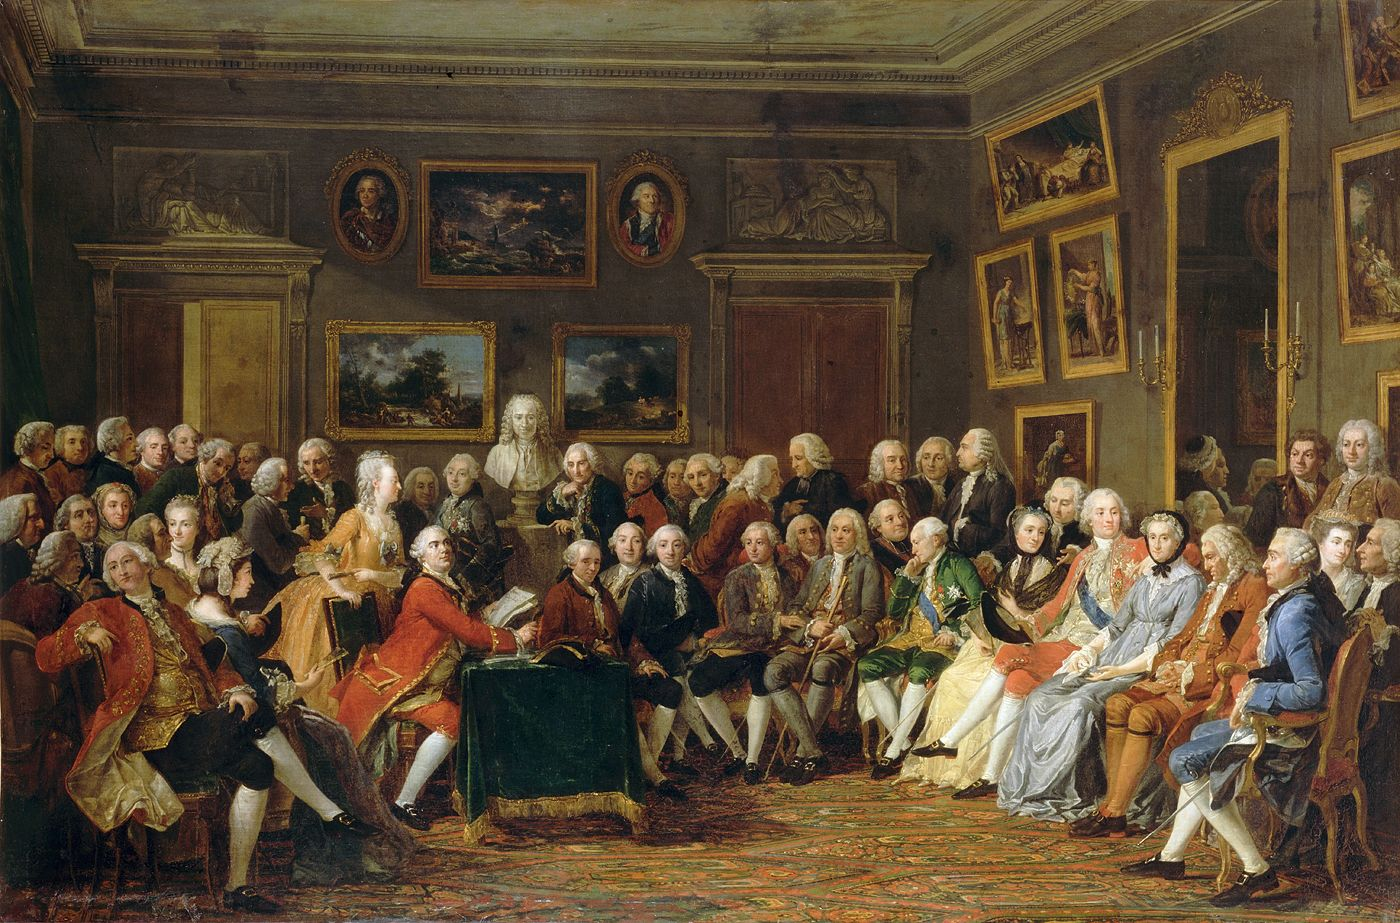
\includegraphics[width=0.75\linewidth]{Les_salons_au_XVIIIe_siècle_-_Histoire_Image.jpg}
    \caption{Enlightenment Period Painting "In the Salon of Madame Geoffrin in 1755."}
    \label{fig:placeholder}
\end{figure}


Regardless of Bayes' original motivation, his work emerged during the English Enlightenment, a period in which philosophers, mathematicians, and scientists increasingly sought to describe uncertainty and rational belief using mathematics. This intellectual movement produced many of the statistical and logical ideas that would later become the foundations of modern probability theory and Bayesian statistics.


%\fcolorbox{red}{red!10}{
 % \textcolor{red}{\textbf{TODO: Add an image of the Enlightenment period.}}
%}

\subsection*{REFERENCES TO BE COMPILED}
McGrayne, S. B. (2011). The Theory That Would Not Die: How Bayes' Rule Cracked the Enigma Code, Hunted Down Russian Submarines, and Emerged Triumphant from Two Centuries of Controversy. Yale University Press.

Stigler, S. M. (1986). The History of Statistics: The Measurement of Uncertainty Before 1900. Harvard University Press.

Hummes book also mentined An Enquiry Concerning Human Understanding



%Short answer is: No.

%But there are stereotypes that Bayes, or more specifically Price, connected the theory with religion - to defend Christian theology as a direct, "more intellectual and rigourous" way to counteract the Scottish Enlightenment philosopher David Hume. (For context: English enlightenment period: from the late 17th century to the late 18th century (roughly 1685 to 1815).

%Bayes instructed his assistance to place a ball in an unknown position on the snooker table and Bayes would throw balls behind his head on the table. The assistant would  then only announce whether the balls landed to the left or to the right of the placed ball. Using this new information bayes would try to predict the where the ball was placed.


\subsection{Laplace's independent search for laws of nature hidden in astronomy data}
By the late eighteenth century, astronomers had collected hundreds of years of observations on the motions of planets such as Jupiter and Saturn. While this gave scientists a huge amount of data to work with, much of it contained observational mistakes, recording errors, and inconsistencies. These errors made it seem as though the planets did not always follow Newton's laws of motion. Instead of assuming Newton's theory was wrong, Pierre Simon Laplace (1749–1827) looked for a way to separate the true motion of the planets from errors in the data.

INCLUSE THE THEORY BEFORE THAT JUPITER AND SATURN WOULD CRASH INTO EACH OTHER

Although Thomas Bayes first introduced the theorem that is now named after him, it was Laplace who independently developed and mathematically formalised the theory. His work was much more rigorous and widely recognised, which is why some historians argue that it should really be known as the Bayes–Laplace theorem.

REFERENCE 
Stigler, S. M. (1986). The history of statistics: The measurement of uncertainty before 1900. Harvard University Press.

Laplace's main contribution was what became known as inverse probability. Traditional or forward modelling asks, "If this model is correct, what data should we observe?" Laplace turned this around and instead asked, "Given all of this observed data, what model most likely produced it, what are the model parameters, and how certain can we be about them?" This was a major shift because it focused on learning from data instead of simply testing a model.


\fcolorbox{red}{red!10}{
  \textcolor{red}{\textbf{TODO: Add an image of the Laplace theorem found in google images CHECK IF EVE HAS ANY PICs.}}
}

His approach helped explain that many of the differences between observations and Newton's predictions were due to measurement errors rather than problems with the laws of physics. This idea became the foundation of Bayesian inference, which is still widely used today in statistics, machine learning, and many areas of scientific research.


Found link similar to what we are working on 
McGrayne, S. B. (2011). The theory that would not die: How Bayes' rule cracked the enigma code, hunted down Russian submarines, and emerged triumphant from two centuries of controversy. Yale University Press.

Laplace, P.-S. (1774). Mémoire sur la probabilité des causes par les événements. Mémoires de l'Académie Royale des Sciences de Paris. (This is Laplace's first publication introducing inverse probability.)

%Laplace formalised the rigourous mathematical proof of bayes
%The birth of "inverse probability" -- note Laplace was very famous and a rigourous mathematician compared to bayes and price. He formulated the theory mathematically, and some even beleive the theory should be named after him. 

%The initial problems with big data he was strugging to work with - centuries of data aggregation and messy data of the orbits of Jupyter and Saturn --> many mistakes led to misalignment with Newton's laws of motion --> Laplace solved the human error (and other errors) through finding inverse probability. 

%Forward modelling asks: "Given this model, what does out data look like?"

%Laplace asked: " Given i have all this data, what does my model look like? what are my model parameters and what is the probability of uncertainty that these parameters are true?"

\subsection{So what is Bayes' theorem?} 

The previous sections introduced the historical origins of Bayesian reasoning through the work of Thomas Bayes and Pierre-Simon Laplace. However, the theorem itself is often presented as a mathematical formula without explaining the intuition behind it. 
MAYBE CHANGE WHST YOU WROTE
In reality, Bayes' theorem is simply a rule for updating probabilities when new information becomes available. Rather than treating probability as fixed, Bayesian inference allows beliefs to change as evidence accumulates.

Before introducing Bayes' theorem, it is first necessary to understand the concept of conditional probability.

Conditional probability measures the probability of an event occurring given that another event has already occurred. Suppose two events, (A) and (B), are defined. The conditional probability of event (A) occurring given that event (B) has occurred is written as (P(A|B)) and is defined as
\begin{equation}
[
P(A|B)=\frac{P(A\cap B)}{P(B)}.
]
\end{equation}

This definition states that once event (B) has occurred, the original sample space is restricted only to outcomes contained within (B). The probability of (A) must further be recalculated within this reduced set of possibilities.

The same joint probability may also be written in the opposite direction,
\begin{equation}
[
P(B|A)=\frac{P(A\cap B)}{P(A)}.
]
\end{equation}

Since both equations describe the same joint event (P(A|B)), they can be equated,
\begin{equation}
[ 
P(A|B)P(B)=P(B|A)P(A),
]
\end{equation}
which, after rearranging, gives Bayes' theorem,
\begin{equation}
    [P(A|B)=\frac{P(B|A)P(A)}{P(B)}.]
\end{equation}

The theorem contains four quantities, each with a seperate interpretation:
\begin{itemize}
    \item \textbf{Prior probability (P(A)):} the initial belief about an event before observing new evidence.
\end{itemize}   
\begin{itemize}
    \item \textbf{Likelihood (P(B|A)):} the probability of observing the evidence assuming the hypothesis is true.
\end{itemize}   
\begin{itemize}
    \item \textbf{Evidence (P(B)):} the overall probability of observing the evidence.
\end{itemize}
\begin{itemize}
    \item \textbf{Posterior probability (P(A|B)):} the updated belief after incorporating the evidence.
\end{itemize}

To summarise, rather than introducing a completely new probability, Bayes' theorem simply redistributes existing probabilities using newly acquired information. This process of continually updating beliefs is known as Bayesian inference.
\subsubsection{A geometric interpretation}

Although Bayes' theorem is usually introduced algebraically, it is often easier to understand geometrically. Imagine a rectangle representing an entire population. The width of the rectangle corresponds to the prior probability (P(A)), while the remaining width represents the complement of the event. The rectangle is then divided horizontally according to whether the observed evidence occurs. The overlapping region corresponds to the joint probability $(P(A\cap B)).$

\fcolorbox{red}{red!10}{
  \textcolor{red}{\textbf{TODO: Add an image of the Geometric interpretation of Bayes' theorem showing prior probability, likelihood and posterior probability}}
}

Viewed geometrically, Bayes' theorem asks a remarkably simple question:
\begin{quote}
    Of all the individuals for whom the evidence is true, what proportion actually belong to the hypothesis being investigated?
\end{quote}

Consequently, the posterior probability is obtained by dividing the area of the overlap by the total area representing the observed evidence. This geometric perspective illustrates that Bayes' theorem is not merely an algebraic identity but a natural consequence of partitioning probability space.

\subsubsection{The Medical paradox}
One of the most famous demonstrations of Bayes' theorem is the medical testing paradox. It highlights why intuitive reasoning about probabilities often leads to incorrect conclusions.

Suppose a disease affects only 1\% of the population. A medical test correctly identifies an infected patient 99\% of the time (99\% sensitivity) and correctly identifies a healthy patient 95\% of the time (95\% specificity).

Many people assume that receiving a positive test result means there is approximately a 99\% chance they have the disease. Bayes' theorem shows that this conclusion is incorrect because it ignores the rarity of the disease.

\fcolorbox{red}{red!10}{%
  \parbox{\dimexpr\linewidth-2\fboxsep-2\fboxrule\relax}{%
    \raggedright
    \textcolor{black}{%  
      \begin{enumerate}
        \itembf To illustrate this, imagine testing 10,000 people.
        \item Approximately 100 people genuinely have the disease.
        \item The test correctly identifies 99 of these individuals.
        \item The remaining 9,900 people are healthy.
        Since the false positive rate is 5\%, approximately 495 healthy people will also receive a positive result.
      \end{enumerate}
    }%
  }%
}%

Therefore, there are
\begin{equation}
    99+495=594    
\end{equation}

positive test results in total, yet only 99 correspond to genuine cases.
The probability that a person actually has the disease after receiving a positive result is therefore

$\frac{99}{594}$
$\approx0.167.$

In other words, despite the test appearing highly accurate, the probability that a positive result indicates genuine disease is only about 16.7\%. The overwhelming number of healthy individuals means that false positives dominate the positive test results.


\fcolorbox{red}{red!10}{
  \textcolor{red}{\textbf{TODO: Add an image of a Frequency tree about the medical testing paradox}}}

This phenomenon demonstrates one of the most important principles of Bayesian inference: evidence cannot be interpreted in isolation.
The strength of new evidence depends critically on the prior probability of the event under investigation. 
Ignoring the prior often leads to serious errors in judgement, a mistake known as the base-rate fallacy.
Bayes' theorem therefore provides much more than a mathematical identity.
It offers a principled framework for learning from evidence by continuously refining beliefs as additional information becomes available. 
This seemingly simple idea would later become the mathematical foundation of modern Bayesian statistics, probabilistic machine learning, artificial intelligence, medical diagnosis, robotics, and countless other applications explored throughout the remainder of this chapter.

NEED HELP WITH THE ALIGNMENT
%Here was explain the theorem in practice with simple examples from : 
%Explain conditional probability then bayes theorem GEOMETRICALLY

%https://www.3blue1brown.com/lessons/bayes-theorem/ 
%+ Proof
%https://youtu.be/U_85TaXbeIo?si=B8yTYpSsGEeVEBOe 
%The medical test paradox, and redesigning Bayes' rule: USE IMAGES
%https://youtu.be/lG4VkPoG3ko?si=jxpWbi86mc0MeRBM


\subsection{Bayesian developments after 1950's} 
Despite strong criticism from Ronald Fisher and many frequentist statisticians, Bayesian statistics continued to develop throughout the twentieth century. Frequentists argued that probability should only describe long run frequencies of repeated events and rejected the idea of assigning probabilities to unknown parameters. However, Bayesian researchers believed probability could also represent uncertainty about unknown quantities, allowing prior knowledge to be combined with observed data. By the 1950s, this debate had led to two major branches of Bayesian statistics: Bayesian inference and Bayesian decision theory.

Bayesian inference focused on updating beliefs using Bayes' theorem. Starting with a prior distribution, new evidence is incorporated through the likelihood function to produce a posterior distribution, representing updated beliefs about the unknown parameters. During this period, Harold Jeffreys made important contributions by introducing objective Bayesian methods. His most well known contribution, Jeffreys prior, provided a way of choosing non-informative priors using the Fisher information matrix, allowing Bayesian analyses to be performed with minimal subjective assumptions. Alongside this, statisticians continued to investigate different choices of informative and non-informative priors, including the uniform prior originally suggested by Laplace.
%(Jeffreys, 1939)

At the same time, Bayesian decision theory developed alongside advances in statistical decision theory. Abraham Wald established the mathematical foundations of decision theory during the 1940s while working on military problems for the United States during the Second World War. One of the famous examples was the aircraft survival problem, where Wald demonstrated that armour should be placed where returning aircraft showed the least damage, since aircraft hit in those locations were less likely to survive. His work introduced the concept of minimising expected loss when making decisions under uncertainty. 
%(Wald, 1950).
article: https://medium.com/@penguinpress/an-excerpt-from-how-not-to-be-wrong-by-jordan-ellenberg-664e708cfc3d

\begin{figure}
    \centering
    
\includegraphics[width=0.4\linewidth]{images.jpeg}
    \caption{Aircraft Survivability Diagram}
    \label{fig:placeholder}
\end{figure}



Leonard J. Savage later combined Wald's statistical decision framework with Bayesian probability. In The Foundations of Statistics (1954), Savage argued that rational decisions should be based on posterior probabilities together with a utility or loss function. Rather than selecting the most likely outcome alone, Bayesian decision theory chooses the action that minimises expected loss or maximises expected utility. This framework closely links to utility theory and provides a practical extension of Bayesian inference from estimating unknown quantities to making optimal decisions.


Today, these two branches are rarely separated. Modern Bayesian methods first use inference to estimate a posterior distribution and then apply decision theory to determine the optimal action. This combination forms the basis of many artificial intelligence and machine learning systems, where posterior distributions quantify uncertainty while loss functions guide decision making. Applications now span medicine, economics, robotics, autonomous systems, and natural language processing, demonstrating how Bayesian inference and Bayesian decision theory together provide a principled framework for learning from data and making decisions under uncertainty.


These developments also laid the foundations for probabilistic reasoning in computing. During the 1930s, Alan Turing studied at Princeton University, where he became acquainted with John von Neumann, whose work on computing and game theory would later complement Bayesian ideas about rational decision making. At the same time, Turing was familiar with Harold Jeffreys' work on probability, and these ideas would later influence his approach to reasoning under uncertainty during the Second World War. This connection provides a natural transition from the theoretical development of Bayesian statistics to one of its earliest practical applications: Turing's Bayesian methods for breaking the German Enigma cipher at Bletchley Park.

CHECK WITH IVE IF ANY INFO IS REPEATED


%Bayesian methods contiued to be developed and attempted to be enhanced regardless of Fishers and other frequentist statisticians protests and refusal to acknowledge the concepts. 
%In the 1950's, 2 branches of bayes were developed. Bayesian inference and bayesian Decision theory. -> Both of which were later combined to make optimal decisions in modern bayesian applications like, economics, medicine and more.

%Looking specifically at Bayesian Decision Theory Branch 1:
%Wald worked with the US on aircraft armors where he used the general stats decision theory. - Aircraft survival experiment
%Savage in 1970's worked on formal bayesian statistical decsion theory

%Decision theory - bayes risk function vs frequentist risk. Link to utility theory example in LLN and CLT chapters. 
%Modern AI systems use both branches- Bayesian inference + Posterior distribution + Decision theory (Loss functions, Expected utility) = optimal decision making

%Branch 2:
%Jefferies prior - Fisher info matrix
%Laplace prior? Informative and non-informative?
%Work  that ties to Alan Turing's work


%% ------------------------------------------
%% ------------------------------------------
% \subsection{Alan Turing and Joan Clarke: Breaking the Enigma}

% Alan turing and von neumann -- alan rivarly 

% jeffrey and Neumann were friends -- jeffrey worked in the priors neumann worked on implosion-type nuclear weapons. aka the manhattan project.. 

% leave jeffrey to previous subsection

% Mention the popularity growth of bayesian methods post publishing her book - "The Theory That Would Not Die.", published May 17, 2011 by historian Sharon Bertsch McGrayne. She played a crucial role in sparking more interest and research into the theory of bayesiam methods. 

% Explain methods from: 
% https://www.youtube.com/watch?v=82q3uYw6MuY&t=813s 
% https://en.wikipedia.org/wiki/Joan_Clarke 

%% Start, updated 21-07-2026 ------------------------------------------

\subsection{WWII Bayes: Turing, Good, Clarke and the Enigma Problem}
\label{sec:wwii-turing-good-clarke}

Although Bayesian methods had already found applications in astronomy, geodesy, insurance and scientific inference during the nineteenth and early twentieth centuries   \cite{mcgrayne2011,hacking1975,franklin2001}, the Second World War provided one of their most remarkable practical successes. 

Building upon initial foundational breakthroughs by Polish mathematicians, the cryptanalysts at Bletchley Park- including Alan Turing, I.~J.~Good and Joan Clarke—developed sophisticated statistical methods for extracting military intelligence from encrypted German communications transmitted using the Enigma cipher machine \cite{hodges2014,hinsley1993}. Their work not only contributed significantly to Allied codebreaking efforts, but also demonstrated how probabilistic reasoning could be used to solve large-scale inference problems under uncertainty. These developments would later influence both modern Bayesian statistics and the early history of computing.

The methods used to break the codes were classified as military secrets for a long time before Turing's assistants (like I.J. Good) introduced these ideas into the public statistical and computer science communities. In the book The Theory That Would Not Die \cite{mcgrayne2011}, science writer Sharon Bertsch McGrayne describes in detail Alan turing's contributions in a critical way such as  Banburismus; the decibans, sequential analysis and Bayes factors; search trees \& species sampling, and others (see \cite{zabell2023secret}).

\subsubsection*{The Problem: Breaking the Enigma Cipher}

The Enigma machine encrypted plaintext by passing each typed letter through a series of rotating electrical rotors before illuminating the corresponding ciphertext letter. Since the rotor positions changed after every key press, and the daily rotor order, ring settings and plugboard connections were changed every twenty-four hours, the number of possible machine configurations was enormous. Testing every configuration was computationally impossible within the time available before the next day's settings came into effect.

\fcolorbox{red}{red!10}{
  \textcolor{red}{\textbf{TODO: Add an image of the Enigma machine. why was frequentist methods useless?}}
}

Rather than searching blindly through every possible key, the aim for the cryptanalysts was to rank competing hypotheses according to how well they explained the observed evidence. The evidence included probable plaintext words (\emph{cribs}), \cite{hodges2014} such as those found in routine weather reports, repeated message formats, operator mistakes, known military terminology, and information obtained from previously decrypted communications, see \cite{kahn1996,hinsley1993}. Each additional clue altered the plausibility of different Enigma settings.

The central statistical question therefore became

\begin{quote}
\itshape
``Given all of the evidence collected so far, which Enigma configuration is now the most probable?''
\end{quote}

\subsubsection*{Key Contributors}

\begin{itemize}
    \item \textbf{Marian Rejewski, Jerzy Różycki, and Henryk Zygalski:} The Polish Biuro Szyfrów mathematicians who made the initial mathematical breakthroughs in the 1930s. Rejewski applied permutation theory to reconstruct the Enigma wiring, and the team built the first electromechanical \emph{Bomba} machines. Their pre-war discoveries and sharing of techniques with Allied intelligence in 1939 provided the foundational architecture for Bletchley Park's work. 
    
    \item \textbf{Alan Turing (1912--1954):}
    While the Polish mathematicians used a more pure algebraic/group-theoretic codebreaking approach, due to the German military changing their security protocols in 1938-39, the team in Bletchley took over. Turing formulated the statistical foundation of Banburismus, introducing sequential likelihood updating and logarithmic weights of evidence to reduce the computational workload on electromechanical Bombe machines. 
    \item \textbf{Irving John (Jack) Good (1916--2009):} Served as Turing's main statistical assistant, later formalising these wartime procedures into mainstream Bayesian theory and subjectivist probability \cite{good1950,good1983}.
    \item \textbf{Joan Clarke (1917--1996):} A leading cryptanalysts in Hut 8 who spearheaded the practical application of Banburismus to complex Naval Enigma (\emph{Dolphin}) traffic.
\end{itemize}

% Today this is known as the problem of Bayesian inference: beliefs about competing hypotheses are updated sequentially as new evidence becomes available.

% \subsubsection*{The Mathematicians Behind the Solution}

% \fcolorbox{red}{red!10}{
%   \textcolor{red}{\textbf{TODO: Add breakthrough made by Polish mathematicians (Marian Rejewski, Jerzy Różycki, and Henryk Zygalski), who provided the initial mathematical framework (permutations, initial Bomba concepts, and rotor wiring) before Bletchley Park took over.}}
% }


% Several mathematicians contributed to the statistical methods used at Bletchley Park, most notably Alan Turing (1912--1954), Irving John (Jack) Good (1916--2009), and Joan Clarke (1917--1996).

% Alan Turing developed statistical procedures for ranking competing Enigma settings according to the available evidence rather than treating cryptanalysis as a purely logical exercise. His work on the Banburismus, a sequential Bayesian procedure, introduced the idea that each new observation contributes a measurable ``weight of evidence'' in favour of one hypothesis over another.

% Jack Good later formalised many of these statistical ideas and explicitly interpreted them within the Bayesian framework. Following the war, Good became one of the principal advocates of Bayesian statistics and helped establish its modern theoretical foundations.

% Joan Clarke was one of the leading cryptanalysts at Bletchley Park and played an important role in applying these statistical methods to German Naval Enigma traffic. Although she did not publish new Bayesian theory herself, her mathematical work formed an essential part of the practical implementation of wartime cryptanalysis.

\subsubsection*{Testing Hypotheses via Decibans}


\textcolor{red}{Introduce base of bayesian hypothesis testing with the textbooks:  \& compare in brief sentence why it is different to freuqentist approaches. When do we use one over the other?}
\noindent
\fcolorbox{red}{red!10}{%
  \parbox{\dimexpr\linewidth-2\fboxsep-2\fboxrule\relax}{%
    \raggedright
    \textcolor{red}{%
      \textbf{TODO:} Add an introduction textbooks about Bayesian Hypothesis testing - mentioning credible intervals vs confidence intervals, use cases - spam emails etc. 
      
      \begin{enumerate}
        \item Statistical Decision Theory and Bayesian Analysis by James O. Berger  
        \item The Bayesian Choice by Christian P. Robert
        \item Bayesian Data Analysis (BDA3) by Andrew Gelman et al.
      \end{enumerate}
    }%
  }%
}

% Suppose $H$ denotes the hypothesis that a particular Enigma setting is correct, while $E$ represents newly observed evidence obtained from an intercepted message.

% Turing and his colleagues preferred to work with \emph{odds}. The prior odds $O(H)$ of a hypothesis $H$ vs. the alternative hypothesis $\neg H$ are defined as

% \begin{equation}
% O(H)
% =
% \frac{\mathbb{P} (H)}
%      {\mathbb{P}(\neg H)}.
% \end{equation}

% Jack Good, who worked directly with Turing at Bletchley Park, details the procedure of weight of evidence in \cite{good1950,good1983}: after observing evidence $E$, (the data), the posterior odds given some observations become

% \begin{equation}
% O(H\mid E)
% =
% O(H)
% \,
% \frac{\mathbb{P}(E\mid H)}
%      {\mathbb{P}(E\mid \neg H)}.
% \end{equation}

% The multiplicative term

% \begin{equation}
% B
% =
% \frac{\mathbb{P}(E\mid H)}
%      {\mathbb{P}(E\mid \neg H)}
% \end{equation}

% is now known as the \emph{Bayes factor}. Each new piece of evidence simply multiplies the current odds, allowing information from many independent clues to accumulate naturally.

% To speed up and simplify repeated manual calculations, Turing introduced the idea of taking logarithms of the odds, or turning probabilities into "decibans". Writing

% \begin{equation}
% W
% =
% \log
% \left(
% \frac{\mathbb{P}(E\mid H)}
%      {\mathbb{P}(E\mid \neg H)}
% \right),
% \end{equation}

% \noindent  each observation contributes an additive quantity known as its \emph{weight of evidence}. Turing measured this quantity using units called \emph{bans}, while smaller units became known as \emph{decibans}. Instead of multiplying many likelihood ratios together, cryptanalysts simply added the corresponding weights of evidence.

% This simple transformation dramatically reduced the computational effort required for hand calculations and became one of the key statistical ideas behind the Banburismus procedure.

% While Banburismus itself was a technique created specifically for Enigma and was officially discontinued in September 1943, the theoretical framework behind it had a direct impact on many problems postwar such as cryptography, some linguistic phenomena, the rise of the Good-Turing estimator that calculates the total probability of encountering any object from any species that has never been seen before in your sample and also became a foundational pillar of n-gram language models
% \cite{zabell2023secret,gale1995good, dallmissing, mcallester2000convergence, avasthi2021processing}. 

Let $H$ denote the hypothesis that a specific Enigma configuration is correct, and let $\neg H$ be its complement. Given initial prior odds,
\begin{equation}
O(H) = \frac{\Pr(H)}{\Pr(\neg H)},
\end{equation}
the observation of new evidence $E$ updates the odds to posterior odds $O(H \mid E)$ via Bayes' theorem:
\begin{equation}
O(H \mid E) = O(H) \cdot \frac{\Pr(E \mid H)}{\Pr(E \mid \neg H)}.
\end{equation}

The multiplicative term $B = \frac{\Pr(E \mid H)}{\Pr(E \mid \neg H)}$ is the \emph{Bayes factor} (or likelihood ratio). To simplify manual computations, Turing expressed likelihood ratios on a logarithmic scale. Defining the weight of evidence $W$ as:
\begin{equation}
W = \log_{10} \left( \frac{\Pr(E \mid H)}{\Pr(E \mid \neg H)} \right),
\end{equation}
cryptanalysts could update belief sequentially through simple addition rather than multiplication:
\begin{equation}
\log_{10} O(H \mid E) = \log_{10} O(H) + W.
\end{equation}

Turing defined a unit of evidence corresponding to a factor of $10$ as a \emph{ban}, and used one-tenth of a ban—a \emph{deciban} ($\text{db}$)—as the working unit. A weight of $1\text{ db}$ represented a factor of $10^{0.1} \approx 1.26$ in odds, roughly the smallest increment of evidence discernable in manual calculations.

\vspace{5mm}

Though Banburismus as a manual procedure was phased out by late 1943 as machine throughput expanded, its foundational concepts laid early groundwork for modern sequential analysis, non-parametric estimation (such as the Good-Turing frequency estimator), and language modeling techniques \cite{zabell2023secret,gale1995good,mcallester2000convergence,avasthi2021processing}.

%% End ------------------------------------------

% add: The Sequential Test \& Wald ConnectionTuring's use of accumulated decibans to reach a decision threshold (stopping rule when $W > \text{threshold}$) is effectively Abraham Wald’s Sequential Probability Ratio Test (SPRT), developed independently in the US around the same time.

\subsection{When Bayes Became Computable: Monte Carlo, Metropolis--Hastings, and Gibbs Sampling}
\label{sec:mcmc-history}

During World War II, Alan Turing and I. J. Good demonstrated that Bayesian updating could be operationalised through sequential evidence weighting—using log-odds, \emph{decibans}, and Good--Turing smoothing to solve cryptanalytic problems under strict mechanical constraints. 

However, these wartime methods relied either on discrete evidence accumulation or continuous analytical approximations. In the post-war decades, as Bayesian inference expanded into complex, high-dimensional parameter spaces $\Theta \subseteq \mathbb{R}^d$, calculating posterior expectations $\mathbb{E}_\pi[h(\theta)] = \int_\Theta h(\theta)\pi(\theta \mid y)d\theta$ required evaluating the marginal likelihood (normalising constant):

\textcolor{red}{Reference to Bayesian into subsection once written up}

\begin{equation}
    p(y) = \int_{\Theta} p(y \mid \theta)\pi_{0}(\theta)\,d\theta.
    \label{eq:marginal-likelihood}
\end{equation}
In high dimensions, standard numerical quadrature scales as $\mathcal{O}(K^d)$ for a grid of size $K$, rendering exact evaluation computationally intractable - the modern problem of the \emph{curse of dimensionality}.

While we will detail a small subsection of the history and methods developed, more details about the history of the MCMC methods can be found in \cite{robert2011short, grimmett2014probability, wiki:mcmc, wiki:metropolishastings}


\noindent
\fcolorbox{red}{red!10}{%
  \parbox{\dimexpr\linewidth-2\fboxsep-2\fboxrule\relax}{%
    \raggedright
    \textcolor{red}{%
      \textbf{TODO:} Add
      
      \begin{enumerate}
        \item overall examples of where mcmc methods are used today - locating the flight?
        \item maybe more details about what inference is vs bayesian inference and why we need it? -> what do 18yo students actually know about this?
        \item explaining in simple terms the consequences of the theorems + their connection to CLT --> elaborate further + add proofs from books + mention Markov Chains intro 1040s
        \item Links to the full algorithms in appendix or code on github. 
        \item any images of the mcmc e.g. locality theorem of gibbs. 
        \item link to Markov Chain CLT with metropolis hastings algo --> using it
        \item What is a transition kernel density and what are the conditions for it? 
      \end{enumerate}
    }%
  }%
}

% -----------------------------------------------------------------------------
\subsubsection{Physics Origins: The Metropolis--Hastings Framework (1953--1970)}
\label{subsec:metropolis-hastings}

The computational breakthrough behind modern Markov chain Monte Carlo (MCMC) originated not in statistics, but in physical chemistry. Nicholas Metropolis, Arianna Rosenbluth, Marshall Rosenbluth, Augusta Teller, and Edward Teller \cite{metropolis1953} sought to calculate macroscopic thermodynamic quantities for systems of $N$ interacting particles in $d$ dimensions ($d \in \{2, 3\}$).

Let $x = (x_1, \dots, x_N) \in \mathcal{X}$ denote a spatial configuration with potential energy $E(x)$. At thermodynamic equilibrium, states follow the canonical Boltzmann distribution:
\begin{equation}
    \pi(x) = \frac{\widetilde{\pi}(x)}{Z} = \frac{\exp\left\{-\beta E(x)\right\}}{Z}, \qquad \text{where } \beta = \frac{1}{k_{\mathrm{B}}T}.
\end{equation}
Evaluating expected physical properties $\mathbb{E}_{\pi}[h(X)]$ required computing the ratio of two high-dimensional integrals over the partition function $Z = \int_{\mathcal{X}} \exp\{-\beta E(x)\} dx$. Standard Monte Carlo sampling $X_i \sim \text{Uniform}(\mathcal{X})$ failed because uniform samples in dense states almost always placed particles unrealistically close together, driving $E(x) \to \infty$ and yielding negligible weights $\exp\{-\beta E(x)\} \approx 0$.

To bypass evaluating $Z$, Metropolis et al. (1953) \cite{metropolis1953} introduced a guided random walk using a symmetric proposal distribution $q(y \mid x) = q(x \mid y)$. While published under five authors, historical accounts attribute the mathematical derivation to Marshall Rosenbluth and the implementation on the MANIAC I computer to Arianna Rosenbluth \cite{gubernatis2005}. W. K. Hastings (1970) \cite{hastings1970} generalised this to asymmetric proposals $q(y \mid x) \neq q(x \mid y)$, transforming a physical simulation technique into a general mathematical tool for statistical sampling.

\begin{proposition}[Cancellation of Normalising Constants \cite{robert2004mcmc}]
\label{prop:cancellation-constant}
Let $\widetilde{\pi}(\theta) = p(y \mid \theta)\pi_0(\theta)$ be an unnormalised target density with normalising constant $Z = p(y)$. For any proposal $q(\cdot \mid \theta)$, the Metropolis--Hastings acceptance probability $\alpha_{\mathrm{MH}}(\theta, \theta')$ satisfies:
\begin{equation}
    \alpha_{\mathrm{MH}}(\theta, \theta') = \min\left\{1, \; \frac{\pi(\theta') q(\theta \mid \theta')}{\pi(\theta) q(\theta' \mid \theta)}\right\} = \min\left\{1, \; \frac{\widetilde{\pi}(\theta') q(\theta \mid \theta')}{\widetilde{\pi}(\theta) q(\theta' \mid \theta)}\right\}.
\end{equation}
\end{proposition}

\noindent This cancellation is the foundation of MCMC computation. It allows samples to be drawn from complex target posterior distributions knowing only the unnormalised joint density $p(y \mid \theta)\pi_0(\theta)$, entirely bypassing the intractable high-dimensional integration required to evaluate $p(y)$.

\begin{theorem}[Detailed Balance and Ergodicity \cite{meyn2012mcke, tierney1994}]
\label{thm:mcmc-ergodic}
If a transition kernel $P(x, dy)$ satisfies detailed balance $\pi(dx) P(x, dy) = \pi(dy) P(y, dx)$, then $\pi$ is invariant. Furthermore, if the resulting Markov chain is $\pi$-irreducible, aperiodic, and positive Harris recurrent, then for any $\pi$-integrable function $h$:
\begin{equation}
    \lim_{M \to \infty} \frac{1}{M} \sum_{m=1}^{M} h(X_m) = \mathbb{E}_\pi[h(X)] \quad \text{a.s.}
\end{equation}
\end{theorem}

\noindent Detailed balance theorem offers a tractable, local condition to ensure that the chain preserves the target distribution $\pi$. Ergodicity provides the formal theoretical guarantee that sample path averages will almost surely converge to true posterior expectations as the chain runs infinitely long.

% -----------------------------------------------------------------------------
\subsubsection{Image Restoration and Gibbs Sampling (1984)}
\label{subsec:gibbs-sampling}

Independently of Hastings' statistical formulation, Stuart and Donald Geman (1984) \cite{geman1984} addressed the problem of recovering a clean digital image $F = (F_s)_{s \in \mathcal{S}}$ over a grid $\mathcal{S}$ given noisy observations $G$, via the posterior $\pi(f \mid g) \propto p(g \mid f) \pi_0(f)$.

To capture local spatial correlations, Geman and Geman modeled the prior $\pi_0(f)$ as a Markov Random Field (MRF) over local neighbourhoods $\partial s$.

\begin{theorem}[Hammersley--Clifford Theorem \cite{besag1974spatial, geman1984}]
\label{thm:hammersley-clifford}
A strictly positive random field $F$ on a finite lattice $\mathcal{S}$ is a Markov Random Field if and only if its joint distribution $\pi_0(f)$ is a Gibbs distribution:
\begin{equation}
    \pi_0(f) = \frac{1}{Z} \exp\left\{ -\frac{1}{T} \sum_{C \in \mathcal{C}} V_C(f) \right\},
\end{equation}
where $T > 0$ is temperature, $\mathcal{C}$ is the collection of local pixel cliques, and $V_C(f)$ are clique potential functions.
\end{theorem}

\noindent This theorem builds a crucial theoretical bridge between local spatial specifications and global joint probability fields. It proves that specifying simple, local interactions is mathematically equivalent to defining a valid joint distribution over the entire lattice.

For a lattice of $d$ pixels with $K$ discrete intensity levels, $Z$ involves $K^d$ terms (e.g., $256^{512 \times 512}$), rendering direct evaluation impossible. Geman and Geman introduced what they named the \emph{Gibbs sampler}—in honor of Josiah Willard Gibbs—noting that the full conditional distribution of a pixel $F_s$ given $F_{-s}$ depends solely on its local neighbourhood $\partial s$:
\begin{equation}
    \pi(f_s \mid f_{-s}) = \pi(f_s \mid f_{\partial s}) = \frac{\exp\left\{ -\frac{1}{T} \sum_{C : s \in C} V_C(f) \right\}}{\sum_{u \in \mathcal{F}_s} \exp\left\{ -\frac{1}{T} \sum_{C : s \in C} V_C(u, f_{-s}) \right\}},
\end{equation}


where $F_{-s}$ denotes the values of all pixels on the grid except pixel $s$. By updating each coordinate iteratively from its full conditional distribution, the chain targets the full joint distribution:
\begin{align}
    X_1^{(m+1)} &\sim \pi(x_1 \mid X_2^{(m)}, X_3^{(m)}, \dots, X_d^{(m)}), \\
    &\;\;\vdots \notag \\
    X_d^{(m+1)} &\sim \pi(x_d \mid X_1^{(m+1)}, X_2^{(m+1)}, \dots, X_{d-1}^{(m+1)}).
\end{align}


\begin{proposition}[Gibbs Update as Exact Metropolis--Hastings \cite{robert2004mcmc}]
\label{prop:gibbs-as-mh}
A Gibbs update proposing $y = (y_i, x_{-i}) \sim \pi(y_i \mid x_{-i})$ is equivalent to a Metropolis--Hastings step with acceptance probability identically equal to 1:
\begin{equation}
    \alpha(x,y) = \min\left\{1, \; \frac{\pi(y) q(x \mid y)}{\pi(x) q(y \mid x)}\right\} = \min\left\{1, \; \frac{\pi(x_{-i})\pi(y_i \mid x_{-i}) \cdot \pi(x_i \mid x_{-i})}{\pi(x_{-i})\pi(x_i \mid x_{-i}) \cdot \pi(y_i \mid x_{-i})}\right\} = 1.
\end{equation}
\end{proposition}
\noindent This unifies Gibbs sampling within the broader Metropolis--Hastings framework. It shows that sampling directly from full conditionals avoids rejected moves entirely ($\alpha = 1$), removing the need to manually choose and tune proposal densities.

% -----------------------------------------------------------------------------
\subsubsection{The Mainstream Statistical Revolution and Applications (1987--Present)}
\label{subsec:mcmc-applications}

The bridge between physical/image models and mainstream Bayesian statistics was completed by Tanner and Wong (1987) \cite{tannerwong1987} via \emph{Data Augmentation} for latent variables, and synthesized by Gelfand and Smith (1990) \cite{gelfandsmith1990}. Gelfand and Smith demonstrated that Gibbs sampling could routinely calculate marginal posterior distributions across arbitrary hierarchical Bayesian models.

The subsequent release of declarative MCMC engines like BUGS (Bayesian inference Using Gibbs Sampling) language \cite{gilks1994} laid the foundation for modern probabilistic programming by demonstrating how to specify complex hierarchical statistical models using Markov chain Monte Carlo (MCMC) methods. Key application domains include:

\begin{itemize}
    \item \textbf{Hierarchical Bayesian Models:} Sequential sampling of hyper-parameters and group parameters in multi-level structures \cite{gelman2013bayesian}.
    \item \textbf{Latent Variable \& Missing Data Models:} Treating unobserved states $Z$ as parameters via Data Augmentation to sample from $\pi(\theta \mid z, y)$ and $\pi(z \mid \theta, y)$ \cite{tannerwong1987}.
    \item \textbf{Spatial Statistics \& Image Processing:} Estimating spatial autoregressions and Markov Random Fields in disease mapping and geostatistics \cite{besag1974spatial}.
    \item \textbf{Phylogenetics \& Population Genetics:} Traversing tree topologies and estimating evolutionary rates from genomic sequences \cite{yang2014molecular}.
\end{itemize}



% End, updated 21-07-2026 -----------------------------------------------------------------------------

\subsection{Bayes through time: state-space models, Kalman filtering and particle filters}


Kalman Filters developed for Apollo Space mission:  applied in Apollo navigation.
https://www.youtube.com/watch?v=MMFpaNm-1EI




Standard MCMC assumes a \emph{static} posterior distribution $\pi(\theta \mid y)$. However, when observations arrive sequentially over time ($y_{1:t}$), re-running MCMC at each step $t$ is computationally prohibitive. 

\cite{sequentialMCinvitation2022}

This necessitates \emph{sequential Bayesian filtering}: evaluating $p(x_t \mid y_{1:t})$ recursively via prediction and update steps. The following section explores how exact updates (Kalman Filters) and particle approximations (Sequential Monte Carlo) extend Bayesian inference into time-evolving dynamical systems.

% \subsection{The path from distributions to optimisation: variational methods}

% - women, other countries

% \subsection{Bayesian Statistics powers Generative Language Models}

\newpage

% --- START OF FIT-TO-PAGE DECISION TREE ---
\begin{figure}[htbp]
\centering

% Color Palette
\definecolor{primary}{HTML}{1A365D}    % Deep Blue
\definecolor{decision}{HTML}{2C5282}   % Slate Blue
\definecolor{leaf}{HTML}{276749}       % Forest Green

% Guaranteed page-width fit
\resizebox{\linewidth}{!}{%
\begin{tikzpicture}[
    auto,
    node distance = 0.9cm and 0.8cm,
    font = \sffamily\small,
    % Decision Box (Rhombus/Diamond)
    question/.style = {
        diamond,
        draw=decision,
        fill=decision!12,
        thick,
        text width=2.8cm,
        align=center,
        inner sep=0pt,
        drop shadow={opacity=0.15, shadow xshift=1pt, shadow yshift=-1pt}
    },
    % Algorithm/Leaf Box (Rectangle)
    leaf/.style = {
        rectangle,
        rounded corners=3pt,
        draw=leaf,
        fill=leaf!12,
        thick,
        text width=3.2cm,
        align=center,
        minimum height=0.7cm,
        inner sep=3pt,
        drop shadow={opacity=0.15, shadow xshift=1pt, shadow yshift=-1pt}
    },
    branch/.style = {
        font=\sffamily\bfseries\scriptsize,
        color=primary
    },
    line/.style = {
        draw=primary,
        -Stealth,
        thick
    }
]

% ==================== NODES ====================

% Level 1: Q1 Likelihood
\node [question] (q1) {\textbf{Q1: Likelihood}\\Is $p(x|z)$ computable?};
\node [leaf, left=0.8cm of q1] (lfi) {\textbf{Likelihood-Free Inference}\\Classical ABC / Neural SBI};

% Level 2: Q2 Data Type
\node [question, below=0.8cm of q1] (q2) {\textbf{Q2: Data Type}\\Dynamic / streaming?};

% Branch Q2 -> YES (Streaming Sub-tree)
\node [question, right=0.8cm of q2] (q2a) {\textbf{Q2a: State}\\Continuous or Discrete?};
\node [leaf, above right=0.1cm and 0.8cm of q2a] (hmm) {\textbf{HMM}\\Forward-Backward / Viterbi};

\node [question, below=0.7cm of q2a] (q2b) {\textbf{Q2b: Dynamics}\\Linear \& Gaussian?};
\node [leaf, right=0.8cm of q2b] (kf) {\textbf{Kalman Filter (KF)}};

\node [question, below=0.7cm of q2b] (q2c) {\textbf{Q2c: Dynamics}\\Severity of non-linearity?};
\node [leaf, right=0.8cm of q2c] (ekf) {\textbf{EKF / UKF}};

\node [question, below=0.7cm of q2c] (q2d) {\textbf{Q2d: Parameters}\\Need static params ($\theta$)?};
\node [leaf, right=0.8cm of q2d] (smc) {\textbf{SIR Particle Filter}};
\node [leaf, below=0.3cm of smc] (pmcmc) {\textbf{PMCMC / SMC$^2$}};

% Branch Q2 -> NO (Static Data)
\node [question, below=3.8cm of q2] (q3) {\textbf{Q3: Data Scale}\\Massive dataset ($N > 10^5$)?};

% Branch Q3 -> YES (Massive N)
\node [question, right=0.8cm of q3] (q3a) {\textbf{Q3a: Latents}\\High-D continuous generative model?};
\node [leaf, above right=0.1cm and 0.8cm of q3a] (vae) {\textbf{Amortized VI (VAE)}};
\node [leaf, below right=0.1cm and 0.8cm of q3a] (svi) {\textbf{Stochastic VI / SGLD}};

% Branch Q3 -> NO (Moderate/Small Data)
\node [question, below=1.8cm of q3] (q4) {\textbf{Q4: Parameters}\\Continuous or Discrete?};

% Branch Q4 -> Discrete
\node [question, right=0.8cm of q4] (q4a) {\textbf{Q4a: Target}\\Multimodal / Combinatorial?};
\node [leaf, above right=0.1cm and 0.8cm of q4a] (asmc) {\textbf{Annealed SMC}};
\node [leaf, below right=0.1cm and 0.8cm of q4a] (gibbs) {\textbf{Gibbs / MH}};

% Branch Q4 -> Continuous
\node [question, below=1.6cm of q4] (q4b) {\textbf{Q4b: Dimension}\\High-D ($D > 20$) or Correlated?};
\node [leaf, right=0.8cm of q4b] (hmc) {\textbf{HMC / NUTS}\\($\nabla_z \log p(x,z)$)};
\node [leaf, below=0.3cm of hmc] (rwm) {\textbf{Random-Walk MH / Slice}};


% ==================== PATHS & CONNECTIONS ====================

% Main Spine
\draw [line] (q1) -- node [branch, left] {NO} (lfi);
\draw [line] (q1) -- node [branch, right] {YES} (q2);
\draw [line] (q2) -- node [branch, right] {NO (Static)} (q3);
\draw [line] (q3) -- node [branch, right] {NO} (q4);

% Dynamic Branch (Q2)
\draw [line] (q2) -- node [branch, above] {YES} (q2a);
\draw [line] (q2a) |- node [branch, near start, above] {Discrete} (hmm);
\draw [line] (q2a) -- node [branch, right] {Continuous} (q2b);
\draw [line] (q2b) -- node [branch, above] {YES} (kf);
\draw [line] (q2b) -- node [branch, right] {NO} (q2c);
\draw [line] (q2c) -- node [branch, above] {Mild} (ekf);
\draw [line] (q2c) -- node [branch, right] {Severe} (q2d);
\draw [line] (q2d) -- node [branch, above] {NO} (smc);
\draw [line] (q2d) |- node [branch, near start, right] {YES} (pmcmc);

% Massive Scale Branch (Q3)
\draw [line] (q3) -- node [branch, above] {YES} (q3a);
\draw [line] (q3a) |- node [branch, near start, above] {YES} (vae);
\draw [line] (q3a) |- node [branch, near start, below] {NO} (svi);

% Parameter Space Branches (Q4)
\draw [line] (q4) -- node [branch, above] {Discrete / Mixed} (q4a);
\draw [line] (q4) -- node [branch, right] {Continuous} (q4b);

\draw [line] (q4a) |- node [branch, near start, above] {YES} (asmc);
\draw [line] (q4a) |- node [branch, near start, below] {NO} (gibbs);

\draw [line] (q4b) -- node [branch, above] {YES} (hmc);
\draw [line] (q4b) |- node [branch, near start, right] {NO} (rwm);

\end{tikzpicture}%
}
\caption{Master Decision Tree for Selecting Bayesian Inference Methods.}
\label{fig:bayes_decision_tree}
\end{figure}
% --- END OF FIT-TO-PAGE DECISION TREE ---

\newpage



\subsection{Dark side of Bayes Theorem vs additional Bayes developments?}

Sally Clark 
https://theconversation.com/bayes-theorem-the-maths-tool-we-probably-use-every-day-but-what-is-it-76140


Data Privacy Issues - inverse engineer NHS data.
-- cases where somehting has happened 

neuclear weapon from Neumann.. 

medical paradox - https://www.youtube.com/watch?v=lG4VkPoG3ko 








\section{The Theory that would not die: Bayesian Probability}\label{sec:bayes}


\noindent
What do guiding NASA's \textbf{Apollo missions} to the Moon, locating the wreckage of \textbf{Air France Flight 447}\footnote{
A useful contrast is the search for Malaysia Airlines Flight MH370. Bayesian methods were also used to estimate probable flight trajectories and crash locations from sparse radar and satellite observations \cite{davey2016bayesian}. Unlike Air France Flight 447, however, these estimated search regions did not lead to recovery of the aircraft's main wreckage. For Air France 447, investigators faced a comparatively constrained search-location problem, whereas for MH370 they first had to infer an unobserved flight trajectory from sparse and indirect measurements before estimating where the aircraft may have entered the ocean.
} in the Atlantic Ocean (\textit{2011}) \cite{stone2014search, cornell2015bayes}, and improving \textbf{Google DeepMind's AlphaGo} before its historic victory over Lee Sedol (\textit{March 2016}) \cite{silver2016mastering} have in common?

\vspace{0.2em}

The answer lies in \textbf{Bayesian statistics}. From recursive state estimation in spacecraft navigation, through Bayesian search theory, to Bayesian optimisation in artificial intelligence, the underlying question for these problems is similar: \textit{"How should uncertain beliefs be revised as new evidence arrives?"}. 

\vspace{0.4em}

This chapter follows the developments of the 18th-century theorem and how it evolved into one of the most powerful computational tools in modern applied mathematics.

\subsection{Was Bayes trying to calculate the existence of God in the 18th century?}

\noindent\textbf{The intellectual setting.}

\vspace{0.4em}

\textbf{Thomas Bayes} (1702 - 1761) lived during the \textbf{Enlightenment}, an intellectual movement of the seventeenth and eighteenth centuries in which European philosophers, mathematicians, and scientists increasingly emphasised reason, observation, and empirical evidence as ways of understanding both the natural and social world. Questions that had traditionally belonged largely to philosophy or theology--what\textit{ should we believe? How strong is the evidence for a claim? How certain can we be about an event we did not observe directly?}--were increasingly being examined via empirical observations adding to the developments in mathematics and probability \cite{hacking1975,stigler1986}. Probability itself had developed rapidly from seventeenth-century work on games of chance, particularly through Pascal, Fermat, Huygens, and later Jacob Bernoulli and Abraham de Moivre, see chapter \ref{chapter:four_CLT}. By Bayes' lifetime, probability was therefore beginning to offer a mathematical language not only for games of chance, but for reasoning about \textit{uncertain evidence}.

In 1748, the Scottish philosopher \textbf{David Hume} (1711 - 1776) wrote in his second book \cite{hume1748enquiry}, his ideas about human nature. In particular, the idea that we are more influenced by our feelings than by reason. In \textit{Section X, ``Of Miracles''}, he questioned whether reason and testimony could justify belief in miraculous religious claims. Hume wrote:

\begin{quote}
\itshape
``The \textit{Christian Religion} [...] cannot be believed by any reasonable person without [a miracle]. Mere reason is insufficient to convince us of its veracity.''
\cite{hume1748enquiry}
\end{quote}

His arguments raised a question that has an unmistakably probabilistic character: \textit{How should our confidence in a claim change when new evidence is presented?} It was around the same time of Hume's book publication that \textbf{Thomas Bayes} investigated what would later be called an \textbf{inverse-probability problem}. Bayes did not publish his work during his lifetime. Following his death in 1761, his friend \textbf{Richard Price} (1723 – 1791), a British moral philosopher, Nonconformist minister and mathematician, discovered the manuscript, edited it, and forwarded it to the Royal Society, where it appeared in 1763 as \textit{An Essay towards Solving a Problem in the Doctrine of Chances} \cite{bayes1763essay}. Rather than assuming that the probability of an event was known and predicting what observations should follow, Bayes asked the reverse question: \textit{given repeated observations, what can be inferred about the unknown probability that produced them?}

% \begin{tcolorbox}[
%     title={Bayes' square-table thought experiment},
%     colback=gray!5,
%     colframe=black!70,
%     boxrule=0.6pt,
%     arc=2mm
% ]

\proofbox{
\textbf{Bayes' square-table thought experiment with modern notation.}

Bayes imagined a \textbf{``square table or plane''}\footnote{
For more detailed mathematical and visual explanations of Bayes'
square-table experiment, see Begley \cite{begley2020bayesian} and the
Cheenta Probability Series \cite{cheentaBayesBilliard}. Accessible video demonstrations are also available here \cite{bayesYoutube1,hannahFryMattParkerBayes}.
} on which balls fall
uniformly at random \cite{bayes1763essay}. After rescaling the table to have
length $1$, let $\theta\in(0,1)$ denote the position of the first ball,
measured as the proportion of the table lying to its left. In other words, $\theta$ measures only the distance from the left-hand edge of the table to the point where the first ball lands, expressed as a proportion of the total table length. The vertical position of the ball is ignored. 

\begin{center}
\begin{tikzpicture}[scale=8]

% Main horizontal line
\draw[thick] (0,0) -- (1,0);

% End points
\draw (0,0.025) -- (0,-0.025);
\draw (1,0.025) -- (1,-0.025);

% First ball position
\filldraw (0.42,0) circle (0.012);

% Labels
\node[below=4pt] at (0,0) {$0$};
\node[below=4pt] at (1,0) {$1$};
\node[above=5pt] at (0.42,0) {$b_1$};

% theta marker
\draw[<->] (0,-0.08) -- (0.42,-0.08);
\node[below=2pt] at (0.21,-0.08) {$\theta$};

% 1-theta marker
\draw[<->] (0.42,-0.08) -- (1,-0.08);
\node[below=2pt] at (0.71,-0.08) {$1-\theta$};

% Optional captions
\node[above=14pt] at (0.21,0) {\small success region};
\node[above=14pt] at (0.71,0) {\small failure region};

\end{tikzpicture}
\end{center}

Thus, before observing any subsequent throws, we can assign the unknown horizontal position $\theta$ of the first ball a \textbf{uniform (prior) distribution},

\[
\theta \sim \mathrm{Unif}(0,1)
        \equiv \mathrm{Beta}(1,1).
\]

% In other words, we assume that before observing any additional data, every horizontal position $\theta$ of the first ball is considered equally plausible.

A subsequent ball $b_2$ is called  \textbf{\textit{success}} if it lands to the left of the first ball. Conditional on $\theta$,

\[
X_i \mid \theta \sim \mathrm{Bernoulli}(\theta),
\qquad
P(X_i=1\mid\theta)=\theta.
\]

where $X_i=1$ if the $i$th ball lands to the left of $b_1$, and $X_i=0$
otherwise. After $n$ independent throws, let $S=\sum_{i=1}^{n}X_i$ denote the total number of \textbf{successful throws}. Then the number of balls that land to the left of the initial ball $b_1$ is modelled by

\[
S \mid \theta \sim \mathrm{Binomial}(n,\theta).
\]

% Hence if we throw $n$ balls independently, and each ball has probability $\theta$ of landing to the left of $b_1$, then $S$ counts how many of those $n$ throws are successful. 
If we observe exactly $S = s$ successful throws, the probability of this outcome, given $\theta$, is

\[
p(s\mid\theta)
=
\binom{n}{s}\theta^{s}(1-\theta)^{\,n-s}.
\]

Note that this conditional density function is viewed as a function of the unknown parameter $\theta$, and it is called the \textbf{likelihood}. Since the factor $\binom{n}{s}$ does not depend on $\theta$, we may write

\[
p(s\mid\theta)
\propto
\theta^{s}(1-\theta)^{\,n-s}.
\]

% Combining this likelihood with Bayes' uniform prior gives

% \[
% p(\theta\mid s)
% \propto
% p(s\mid\theta)p(\theta)
% \propto
% \theta^{s}(1-\theta)^{\,n-s},
% \]

% and therefore, in modern notation,

% \[
% \boxed{
% \theta\mid S=s
% \sim
% \mathrm{Beta}(s+1,n-s+1)
% }.
% \]
Combining the likelihood with the uniform prior using Bayes' rule gives

\[
p(\theta\mid s)
\propto
p(s\mid\theta)p(\theta).
\]

Since the uniform prior satisfies $p(\theta)=1$, $0<\theta<1,$ we obtain

\[
p(\theta\mid s)
\propto
\binom{n}{s}\theta^s(1-\theta)^{n-s}\times 1
\propto
\theta^s(1-\theta)^{n-s}.
\]

Although this has the same mathematical shape as the likelihood, this occurs
because the prior is uniform and therefore contributes no preference towards
any particular value of $\theta$. The observed data now determine how the
posterior probability is distributed across the possible values of $\theta$.
After normalisation,

\[
\theta\mid S=s
\sim
\mathrm{Beta}(s+1,n-s+1).
\]

The \textbf{prior} represents uncertainty about the unknown position before
observing the additional throws; the \textbf{likelihood} records how compatible
each possible value of $\theta$ is with the observations; and the
\textbf{posterior} describes the remaining uncertainty about $\theta$ after
the data have been observed.

}


\paragraph{But was Hume the reason?}
This remains historically uncertain. One interpretation is that Bayes developed inverse probability partly in response to Hume's arguments concerning miracles: perhaps sufficiently strong accumulated evidence could overcome the initially small probability assigned to an extraordinary claim.\textbf{Stephen Stigler} (1941), a professor in Statistics, argues that a connection between Bayes, Price, and contemporary theological debates is plausible \cite{stigler2013truetitle}. While, statisticians Diniz and Bellhouse argue that Bayes' interest was primarily mathematical, arising from problems encountered in de Moivre's \textit{Doctrine of Chances}, rather than from an attempt to refute Hume \cite{diniz2022bayes}. Crucially, there is \textbf{no surviving statement from Bayes confirming that refuting Hume or proving the existence of God was his intention}.

\begin{figure}[H]
\centering
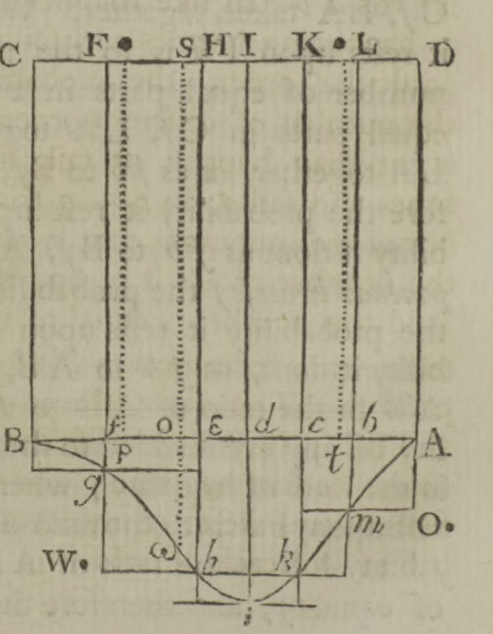
\includegraphics[width=0.35\linewidth]{figs/Bayes_figs/Bayes_Royal_society_Screenshot_illustration.png}
\caption{A modern illustration of Bayes' square-table thought experiment. Bayes described a ``square table or plane'', rather than specifically a billiard or pool table, see \href{https://royalsocietypublishing.org/rstl/article/doi/10.1098/rstl.1763.0053/119736/LII-An-essay-towards-solving-a-problem-in-the}
{Bayes' original 1763 essay}.}
\label{fig:bayes_billard}
\end{figure}


% \subsection{Laplace: From Uncertain Astronomical Observations to Inverse Probability}

\subsection{Laplace: Independently Developing and Extending Inverse Probability}

Thomas Bayes' essay of 1763 had solved a particular inverse problem: after observing a sequence of successes and failures, how could one infer the unknown probability that generated them? Through his square-table construction, Bayes effectively treated the unknown probability as uniformly distributed over $(0,1)$ and then updated this distribution using the observed data.

\textbf{Pierre-Simon Laplace} (1749--1827) independently developed the idea in a more general form. In his 1774 memoir, \textit{Mémoire sur la probabilité des causes par les événements} (``Memoir on the Probability of Causes from Events''), Laplace distinguished between predicting an uncertain event when its cause (a different event) is known and the reverse problem in which the event has been observed but its cause remains unknown \cite{laplace1774,stigler1986laplace}.  As \textbf{Sharon Bertsch McGrayne} summarises it in \textit{The Theory That Would Not Die} (2011),

\begin{quote}
``the probability of a cause (given an event) is proportional to the probability of the event (given its cause).''
\cite{mcgrayne2011}
\end{quote}

Laplace did not state the general principle using modern conditional-probability notation. Instead Laplace's statement appears in Article II of the 1774 memoir, shown in Figure~\ref{fig:laplace_inverse_principle}. He explains that if an observed event can have arisen from several possible causes, then the probabilities assigned to those causes after observing the event should be proportional to the probabilities with which each cause would have produced that event \cite{laplace1774}. Under the assumption that the possible causes are initially equally probable, the principle can be written in modern notation as

\[
P(C_i\mid E)\propto P(E\mid C_i).
\]

\begin{figure}[H]
    \centering
    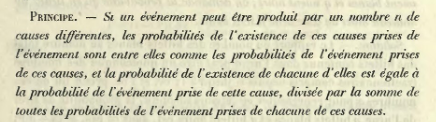
\includegraphics[width=0.5\textwidth]
    {figs/Bayes_figs/Laplace_cause_of_an_event_principle.png}

    \caption{Laplace's statement of his inverse-probability principle in
    Article II of \textit{Mémoire sur la probabilité des causes par les
    événements} (1774); see the
    \href{https://fr.wikisource.org/wiki/Page:Laplace_-_\%C5\%92uvres_compl\%C3\%A8tes,_Gauthier-Villars,_1878,_tome_8.djvu/41}
    {original facsimile}.}

    \label{fig:laplace_inverse_principle}
\end{figure}

% Laplace then applied the principle to his \textit{Problem I} with two urns that contain an infinite number of white and black banknotes in an unknown ratio. If an unknown probability $\theta$ could take any value in $(0,1)$, and $s$ successes and $n-s$ failures had been observed, he obtained an expression equivalent to

% \[
% \frac{\theta^s(1-\theta)^{n-s}\,d\theta}
% {\displaystyle\int_0^1 \theta^s(1-\theta)^{n-s}\,d\theta},
% \]

% \noindent
% for the probability assigned to possible values of $\theta$ after observing the data \cite{laplace1774}. In modern terminology this is the same Beta-type posterior that arises in Bayes' original problem. Laplace's contribution was therefore not simply a rediscovery of Bayes' calculation, but a broader formulation of inverse reasoning that could be applied to unknown causes, parameters and future observations \cite{stigler1986laplace,stigler1986}.

\proofbox{
\textbf{Laplace's urn problem: from past observations to future probability, see also \cite{laplace1774} for more details.}


Laplace illustrated his principle of inverse probability using an urn
containing an infinite number of white and black tickets in an
\textbf{unknown proportion}. 

% Suppose that $\mathbf{p}$ white tickets and $\mathbf{q}$ black tickets have already been observed. If $\mathbf{x}$ \textbf{denotes the unknown proportion of white tickets in the urn}, Laplace assigned the possible values of $x$ a probability proportional to
Suppose that $\mathbf{p}$ white tickets and $\mathbf{q}$ black tickets have already been observed, and let $\mathbf{x}$ denote the \textbf{unknown proportion of white tickets in the urn}.

If the \textbf{true} proportion were $\mathbf{x}$, then in modern notation

\[
P(\text{white ticket}\mid x)=x,
\qquad
P(\text{black ticket}\mid x)=1-x.
\]

Therefore, after observing $p$ white tickets and $q$ black tickets, Laplace associated each possible value of $x$ with the quantity

\[
x^p(1-x)^q.
\]

Thus, $x^p(1-x)^q$ measures how compatible a particular value of $\mathbf{x}$ is with the observations already made.

He then asked a slightly different question from Bayes: \textit{given these past observations, what is the probability that the next ticket drawn will be white?}



For any fixed value of $x$, that probability is simply also just $\mathbf{x}$, as the ratio shouldn't change. However, since $x$ is unknown, \textbf{Laplace considered all possible values of} $\mathbf{x}$ \textbf{between} $\mathbf{0}$ and $\mathbf{1}$, weighting each according to $x^p(1-x)^q$. He denoted the resulting ``entire probability'' by $E$:

\[
E
=
\frac{
\displaystyle\int_0^1
x\,x^p(1-x)^q\,dx
}{
\displaystyle\int_0^1
x^p(1-x)^q\,dx
}
=
\frac{
\displaystyle\int_0^1
x^{p+1}(1-x)^q\,dx
}{
\displaystyle\int_0^1
x^p(1-x)^q\,dx
}.
\]

The denominator ensures that the weights assigned to all possible values of $x$ are properly normalised, while the additional factor $x$ in the numerator accounts for the probability of drawing a white ticket for each possible value of $x$.

Laplace evaluates the integral over a few pages, and gives the answer

\[
\boxed{
E=\frac{p+1}{p+q+2}
}
\]

so $E$ is the probability, inferred from the $p+q$ observations already made, that the \emph{next} ticket drawn from the urn will be white \cite{laplace1774}.
}

\noindent
McGrayne illustrates the difference in scope between Bayes and Laplace with the analogy

\begin{quote}
``If Bayes and Price asked whether today's puddles could tell us whether it had rained yesterday and whether it might rain tomorrow, Laplace asked how much rain might fall and then repeatedly revised that estimate as additional information became available.''
\cite{mcgrayne2011}
\end{quote}

The important extension was the possibility of \textbf{\textit{repeated updating}}: as new observations arrived, the probability assigned to an unknown quantity could be revised again.

Laplace's work on probability soon developed alongside his work in astronomy and celestial mechanics. In Chapter~2, ``The Man Who Did Everything,'' McGrayne describes how eighteenth-century astronomers possessed observations extending over centuries, although the measurements differed greatly in precision and sometimes appeared inconsistent with Newtonian celestial mechanics.\footnote{For examples of astronomical observations available before Laplace, see Flamsteed's \textit{Historia Coelestis Britannica} \cite{flamsteed1725}. For the older European tradition of planetary tables, see Chabás and Goldstein \cite{chabasgoldstein2012}.} One particularly troubling example concerned the apparent long-term motions of Jupiter and Saturn. As McGrayne writes,

\begin{quote}
``...eventually, they thought, Jupiter would smash into the sun, and Saturn would spin off into space.''
\cite{mcgrayne2011}
\end{quote}

Laplace's 1774 memoir had not been written specifically to solve this astronomical problem. Rather, he used probability, theories of observational error and other analytical methods alongside celestial mechanics to infer unknown astronomical quantities from imperfect observations \cite{mcgrayne2011}. Some of Laplace's related contributions to large-sample approximation and probability are discussed in the earlier Chapter~\ref{chapter:four_CLT}.


% \subsubsection*{Why did inverse probability later become controversial?}
% \subsection{What become of this theory in the 19th century?}


\subsubsection*{Inverse probability in the nineteenth century: continued use and growing criticism}

The nineteenth century was a period of rapid expansion in both probability theory and the use of mathematics to analyse empirical observations. As discussed further in Chapter~\ref{chapter:four_CLT}, Laplace developed \textbf{generating functions} and \textbf{normal approximations}; Siméon-Denis Poisson (1781 - 1840) extended the \textbf{theory of repeated trials} and introduced the expression \textbf{law of large numbers}; Irénée-Jules Bienaymé (1796 - 1878) contributed to \textbf{probability inequalities} and \textbf{error theory}; and Pafnuty Chebyshev (1821 - 1894) later established increasingly general results concerning \textbf{averages, inequalities and convergence} \cite{poissonnn1837} \cite{bienayme1853} \cite{chebyshev1867}

% \cite{poisson1837,bienayme1853,chebyshev1867}. 

At the same time, probability and statistical methods were being applied to an expanding range of empirical data. It was beginning to form what we would now recognise as \textbf{statistical methodology}. Astronomers and geodesists continued to estimate unknown quantities from noisy measurements using methods associated with Laplace (1749 - 1827), Legendre (1752 - 1833) and Gauss (1777 - 1855), while Adolphe Quetelet (1796 - 1874) transferred ideas about averages, variation and the normal law from astronomy to large collections of demographic and social observations \cite{stigler1986,gauss1809,quetelet1835}. McGrayne also writes 

\begin{quote}
\textit{" \textbf{James Clerk Maxwell} (1831 - 1879), learned about probability from Adolphe Quetelet (1796 - 1874), not from Laplace, and adopted frequency-based methods for statistical mechanics and the kinetic theory of gases.",} \cite{mcgrayne2011}
\end{quote}


In modern language, the nineteenth century was beginning to face an early version of the \textbf{“big data” problem}: scientists and governments were collecting increasingly large amounts of \textit{astronomical, demographic and social observations}, creating a need for mathematical methods that could identify patterns, quantify uncertainty and estimate unknown quantities from data. During the time inverse probability remained in use, particularly in applied problems of estimation, but it was no longer the only framework through which mathematicians and scientists were learning from uncertain observations.

The theory's biggest difficulty was concerned with the probabilities assigned to unknown causes or parameters. Bayes' construction and many of Laplace's calculations began by treating possible values as \textbf{initially equally probable}. This assumption continued discussions in the 20th century, under the name of \textit{principle of indifference}\footnote{The expression ``principle of indifference'' was used prominently by Keynes in his \textit{Treatise on Probability} (1921); related arguments had long been discussed under the older expression ``principle of insufficient reason''.}. For a symmetric problem such as throwing an idealised fair die, assigning equal probabilities may appear natural. For an unknown planetary mass parameter, population parameter, or other continuous quantity, however, there is no obvious reason why a lack of prior knowledge should imply that we assign equal initial probabilities to the model parameters. George Boole (1815 - 1864) , John Venn (1834 - 1923) and Joseph Bertrand (1822 - 1900) criticised different aspects of this reasoning \cite{boole1854,venn1866,bertrand1889}. In the chapter \textbf{``Many doubts, few defenders''} \cite{mcgrayne2011} McGrayne discusses many arguments noted during the century about Laplace's reasoning.  

While John Maynard Keynes, see \href{https://archive.org/details/treatiseonprobab007528mbp/page/382/mode/2up}{A Treatise on Probability (1921), Chapter XXX, “Statistical Inference”, around pp. 382} states 

\begin{quote}
``...it has been very widely accepted, — by Augustus De Morgan (1806 - 1871), by William Stanley Jevons (1835 - 1882), by Rudolf Hermann Lotze (1817–1881), by Emanuel Czuber (1851 - 1925), and by Professor Pearson, — to name some representative writers of successive schools and periods.''\cite{keynes1921,mcgrayne2011}
\cite{mcgrayne2011}
\end{quote}

 

The controversy was therefore increasingly about the \emph{interpretation} of inverse probability rather than the validity of conditional probability itself: \textbf{could an unknown but fixed quantity legitimately be assigned a probability distribution, and how should that distribution be chosen?} These questions remained unresolved at the end of the nineteenth century. In the early twentieth century they became much sharper as \textbf{alternative theories of statistical inference} were developed. R.~A.~Fisher (1890 - 1926) would reject inverse probability as a general foundation for parameter inference and develop \textbf{likelihood-based methods} that did not require prior probabilities \cite{fisher1922}, while other mathematicians---including Harold Jeffreys (1891 - 1989), \textbf{Dorothy Wrinch} (1894 - 1976)\footnote{\textbf{Dorothy Wrinch} (1894–1976) was a mathematician and philosopher of science, and \textbf{the first woman to receive a Doctor of Science (DSc) degree from Oxford University (awarded in 1929)}. She collaborated with Harold Jeffreys on probability and scientific inference between 1919 and 1923. Their work has been identified as an important conceptual precursor to Bayesian hypothesis testing and the later Bayes factor; Jeffreys subsequently acknowledged Wrinch's substantial contribution to the foundations of his work on scientific inference. \href{https://mathshistory.st-andrews.ac.uk/Extras/Jeffreys_Probability/}{An extract from Jeffreys' book on Probability} \cite{wrinchjeffreys1919,wrinchjeffreys1921,jeffreys1973} } and Bruno de Finetti (1906 - 1985)---would instead attempt to place probabilistic inference on stronger foundations. The resulting disagreement marks the beginning of the much more explicit twentieth-century debate over how statistical inference should be performed.


\subsection{So what is Bayes' theorem today?} 

An excellent introductory Probability book is written by Tijms' \textit{\textbf{Understanding Probability}} \cite{tijms2012}. \textbf{Chapter~8} develops conditional probability, the law of total probability and Bayes' rule before introducing Bayesian statistics for the discrete case. \textbf{Chapter~13} later extends these ideas to continuous random variables and continuous Bayesian models. For readers already comfortable with these probability and calculus concepts, Gelman et al.'s \textit{\textbf{Bayesian Data Analysis}} provides a natural next step \cite{gelman2013bayesian}. 
A visual and intuitive explanation of Bayes' theorem, is provided in several \textbf{YouTube video introductions}, including \textbf{3Blue1Brown}'s \href{https://youtu.be/HZGCoVF3YvM}{geometric explanation of Bayes' theorem}, as well as further examples by \href{https://youtu.be/NLKWLBJ-b9E}{RiskByNumbers} and \href{https://youtu.be/5NMxiOGL39M}{Brandon Rohrer}. 3Blue1Brown also explores Bayes' rule through the \href{https://youtu.be/lG4VkPoG3ko}{medical test paradox}, illustrating visually why base rates and prior probabilities matter when interpreting evidence.

\vspace{2mm}

Modern introductions to Bayes' theorem usually begin with the
\textbf{discrete case}. Suppose that the events $B_1,\ldots,B_k$ represent all possible hypotheses, explanations or parameter values under consideration. For example, in Bayes' experiment, the unknown
quantity was \textbf{the position} $\theta$ \textbf{of the first ball} on the table, while in Laplace's urn problem it was the actual \textbf{unknown proportion} $\mathbf{x}$ \textbf{of white tickets}. These are assumed to be \textbf{mutually exclusive}, so that no two can occur simultaneously, and \textbf{exhaustive}, so that one of them must occur. 

Let $A$ denote some observed evidence, or collected data. In Bayes' experiment, this could be the observation that, among $n$ subsequent balls, $s$ fell to the left of the first ball and $n-s$ to its right. In Laplace's urn problem, the corresponding evidence was the observation of $p$ white tickets and $q$ black tickets. 

Two results from probability theory are needed. First, \textbf{conditional probability}
is defined by

\[
P(B_i\mid A)
=
\frac{P(B_i\cap A)}{P(A)}.
\]

Second, the \textbf{law of total probability} says that the probability of
observing $A$ can be found by considering all the different hypotheses under
which $A$ could have occurred:

\[
P(A)
=
\sum_{j=1}^{k}P(A\mid B_j)P(B_j).
\]

This can be visualised geometrically by dividing the event $A$ into the
mutually exclusive pieces contributed by each possible hypothesis, as shown
in Figure~\ref{fig:total_probability}.

\begin{figure}[H] \centering 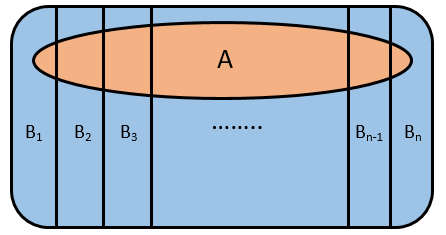
\includegraphics[width=0.45\textwidth]{figs/Bayes_figs/law_total_probability_venn.png} \caption{Geometric illustration of the law of total probability. The sample space is partitioned into mutually exclusive events $B_1,\ldots,B_n$, and the probability of $A$ is obtained by adding its intersections with each part of the partition. Illustration source: \href{https://qualityengineer.weebly.com/probability/total-probability-law}{Blog by Authors: Armin Nikzad and Fatima Mosallaei}.} \label{fig:total_probability} \end{figure}

Since the intersection can also be obtained by $P(B_i\mid A)P(A) = P(B_i\cap A) = P(A\cap B_i) = P(A\mid B_i)P(B_i)$,  substituting the law of total probability into conditional probability gives the modern discrete  form\footnote{Bayes' theorem may appear in different notation or equivalent forms across textbooks, depending on whether it is stated for events, hypotheses, random variables or statistical parameters; the underlying relationship is the same.} of \textbf{Bayes' theorem}:

\begin{equation}
    \boxed{
    P(B_i\mid A)
    =
    \frac{P(A\mid B_i)P(B_i)}
    {\displaystyle
    \sum_{j=1}^{k}P(A\mid B_j)P(B_j)}
    }.
\end{equation}

\noindent
Further details on conditional probability and the law of total probability can be found in \cite{tijms2012}.

In words, Bayes' theorem begins with probabilities assigned to the different possible hypotheses $B_i$, asks how compatible the observed evidence $A$ is with each of them, and then uses this information to revise their probabilities after the evidence has been observed. In modern Bayesian terminology this is often summarised as

\begin{equation}
    \boxed{
    \text{posterior}
    \propto
    \text{likelihood}
    \times
    \text{prior}
    }.
\end{equation}

The same idea extends naturally to \textbf{continuous} problems. In the discrete case there is a finite or countable list of possibilities, $B_1,B_2,\ldots,B_k$. In a continuous problem, however, an unknown quantity may take any value within an interval. For example, an unknown probability might take any value between $0$ and $1$, rather than being restricted to a list of possible values. Such an unknown quantity is commonly represented by a parameter such as $\theta$.

To connect the discrete and continuous forms, let $B_i$ represent the event
that an unknown parameter $\Theta$ takes the value $\theta_i$, suppose that the hypotheses $B_i$ correspond to possible values of an unknown parameter $\Theta$, so that $B_i=\{\Theta=\theta_i\},$ and let the observed evidence $A$ correspond to observing the data $x$.
Then the discrete form of Bayes' theorem, may equivalently be written in parameter notation as

\[
P(\Theta=\theta_i\mid x)
=
\frac{
P(x\mid\theta_i)\,P(\Theta=\theta_i)
}{
\displaystyle
\sum_{j=1}^{k}
P(x\mid\theta_j)\,P(\Theta=\theta_j)
}.
\]

Here the possible parameter values $\theta_1,\ldots,\theta_k$ still form a
finite or countable collection. If $\Theta$ is instead continuous, these individual probability masses are replaced by probability densities, and the sum over the possible values $\theta_j$ becomes an integral over the continuum of possible values of $\theta$. This is the same mathematical transition from summation to integration discussed in the Calculus chapter (see Section~\ref{sec:CALCULUS }).

The continuous form of Bayes' theorem is therefore

\begin{equation}
\boxed{
\overbrace{p(\theta\mid x)}^{\text{posterior density}}
=
\frac{
    \overbrace{p(x\mid\theta)}^{\text{likelihood}}
    \;
    \overbrace{p(\theta)}^{\text{prior density}}
}{
    \underbrace{
    \displaystyle\int p(x\mid u)p(u)\,du
    }_{
    \substack{
    \text{marginal density }p(x)\\
    \text{(evidence / normalising constant)}
    }
    }
}
}.
\label{eq:continuous_bayes}
\end{equation}

Here $u$ is a dummy variable of integration. The denominator sums, or in the
continuous case integrates, over all possible values of the unknown
parameter.


%HELP move diagram below text
% NOTE: INFERENCE IS NOT THE POINT OF THIS SUBSECTION - THIS SECTION JUST EXPLAINS THE CLASSIC BAYES THEOREM. + Notation does not match. It is unnecessarily confusing as not explained. 
% \begin{figure}
%     \centering
%     \includegraphics[width=0.5\linewidth]{Bayesian Process Diagram.png}
%     \caption{Bayesian Inference Process Diagram}
%     \label{fig:placeholder}
% \end{figure}
% If $x$ denotes the observed data, the continuous form of Bayes' theorem can be written as 
% \begin{equation} \boxed{ p(\theta\mid x) = \frac{p(x\mid\theta)p(\theta)} {\displaystyle \int p(x\mid u)p(u)\,du} }. \end{equation}

% Here $p(\theta)$ is the \textbf{prior density}, $p(x\mid\theta)$ is the \textbf{likelihood}, and $p(\theta\mid x)$ is the \textbf{posterior density}. The denominator plays the same role as the sum in the discrete version: it accounts for all possible values of the unknown parameter and normalises the posterior so that it integrates to one. The difference is that, because $\theta$ may take continuously many possible values, the discrete sum is replaced by an integral.


% The previous sections introduced the historical origins of Bayesian reasoning through the work of Thomas Bayes and Pierre-Simon Laplace. However, the theorem itself is often presented as a mathematical formula without explaining the intuition behind it. 
% MAYBE CHANGE WHST YOU WROTE
% In reality, Bayes' theorem is simply a rule for updating probabilities when new information becomes available. Rather than treating probability as fixed, Bayesian inference allows beliefs to change as evidence accumulates.

% Before introducing Bayes' theorem, it is first necessary to understand the concept of conditional probability.

% Conditional probability measures the probability of an event occurring given that another event has already occurred. Suppose two events, (A) and (B), are defined. The conditional probability of event (A) occurring given that event (B) has occurred is written as (P(A|B)) and is defined as
% \begin{equation}
% [
% P(A|B)=\frac{P(A\cap B)}{P(B)}.
% ]
% \end{equation}

% This definition states that once event (B) has occurred, the original sample space is restricted only to outcomes contained within (B). The probability of (A) must further be recalculated within this reduced set of possibilities.

% The same joint probability may also be written in the opposite direction,
% \begin{equation}
% [
% P(B|A)=\frac{P(A\cap B)}{P(A)}.
% ]
% \end{equation}

% Since both equations describe the same joint event (P(A|B)), they can be equated,
% \begin{equation}
% [ 
% P(A|B)P(B)=P(B|A)P(A),
% ]
% \end{equation}
% which, after rearranging, gives Bayes' theorem,
% \begin{equation}
%     [P(A|B)=\frac{P(B|A)P(A)}{P(B)}.]
% \end{equation}

% The theorem contains four quantities, each with a seperate interpretation:
% \begin{itemize}
%     \item \textbf{Prior probability (P(A)):} the initial belief about an event before observing new evidence.
% \end{itemize}   
% \begin{itemize}
%     \item \textbf{Likelihood (P(B|A)):} the probability of observing the evidence assuming the hypothesis is true.
% \end{itemize}   
% \begin{itemize}
%     \item \textbf{Evidence (P(B)):} the overall probability of observing the evidence.
% \end{itemize}
% \begin{itemize}
%     \item \textbf{Posterior probability (P(A|B)):} the updated belief after incorporating the evidence.
% \end{itemize}

% To summarise, rather than introducing a completely new probability, Bayes' theorem simply redistributes existing probabilities using newly acquired information. This process of continually updating beliefs is known as Bayesian inference.


% \subsubsection{A geometric interpretation}

% Although Bayes' theorem is usually introduced algebraically, it is often easier to understand geometrically. Imagine a rectangle representing an entire population. The width of the rectangle corresponds to the prior probability (P(A)), while the remaining width represents the complement of the event. The rectangle is then divided horizontally according to whether the observed evidence occurs. The overlapping region corresponds to the joint probability $(P(A\cap B)).$

% \fcolorbox{red}{red!10}{
%   \textcolor{red}{\textbf{TODO: Add an image of the Geometric interpretation of Bayes' theorem showing prior probability, likelihood and posterior probability}}
% }

% Viewed geometrically, Bayes' theorem asks a remarkably simple question:
% \begin{quote}
%     Of all the individuals for whom the evidence is true, what proportion actually belong to the hypothesis being investigated?
% \end{quote}

% Consequently, the posterior probability is obtained by dividing the area of the overlap by the total area representing the observed evidence. This geometric perspective illustrates that Bayes' theorem is not merely an algebraic identity but a natural consequence of partitioning probability space.

% \subsubsection{The Medical paradox}
% One of the most famous demonstrations of Bayes' theorem is the medical testing paradox. It highlights why intuitive reasoning about probabilities often leads to incorrect conclusions.

% Suppose a disease affects only 1\% of the population. A medical test correctly identifies an infected patient 99\% of the time (99\% sensitivity) and correctly identifies a healthy patient 95\% of the time (95\% specificity).

% Many people assume that receiving a positive test result means there is approximately a 99\% chance they have the disease. Bayes' theorem shows that this conclusion is incorrect because it ignores the rarity of the disease.

% \fcolorbox{red}{red!10}{%
%   \parbox{\dimexpr\linewidth-2\fboxsep-2\fboxrule\relax}{%
%     \raggedright
%     \textcolor{black}{%  
%       \begin{enumerate}
%         \itembf To illustrate this, imagine testing 10,000 people.
%         \item Approximately 100 people genuinely have the disease.
%         \item The test correctly identifies 99 of these individuals.
%         \item The remaining 9,900 people are healthy.
%         Since the false positive rate is 5\%, approximately 495 healthy people will also receive a positive result.
%       \end{enumerate}
%     }%
%   }%
% }%

% Therefore, there are
% \begin{equation}
%     99+495=594    
% \end{equation}

% positive test results in total, yet only 99 correspond to genuine cases.
% The probability that a person actually has the disease after receiving a positive result is therefore

% $\frac{99}{594}$
% $\approx0.167.$

% In other words, despite the test appearing highly accurate, the probability that a positive result indicates genuine disease is only about 16.7\%. The overwhelming number of healthy individuals means that false positives dominate the positive test results.


% \fcolorbox{red}{red!10}{
%   \textcolor{red}{\textbf{TODO: Add an image of a Frequency tree about the medical testing paradox}}}

% This phenomenon demonstrates one of the most important principles of Bayesian inference: evidence cannot be interpreted in isolation.
% The strength of new evidence depends critically on the prior probability of the event under investigation. 
% Ignoring the prior often leads to serious errors in judgement, a mistake known as the base-rate fallacy.
% Bayes' theorem therefore provides much more than a mathematical identity.
% It offers a principled framework for learning from evidence by continuously refining beliefs as additional information becomes available. 
% This seemingly simple idea would later become the mathematical foundation of modern Bayesian statistics, probabilistic machine learning, artificial intelligence, medical diagnosis, robotics, and countless other applications explored throughout the remainder of this chapter.

% NEED HELP WITH THE ALIGNMENT
%Here was explain the theorem in practice with simple examples from : 
%Explain conditional probability then bayes theorem GEOMETRICALLY

%https://www.3blue1brown.com/lessons/bayes-theorem/ 
%+ Proof
%https://youtu.be/U_85TaXbeIo?si=B8yTYpSsGEeVEBOe 
%The medical test paradox, and redesigning Bayes' rule: USE IMAGES
%https://youtu.be/lG4VkPoG3ko?si=jxpWbi86mc0MeRBM


% \subsection{Bayesian developments after 1950's} 


% \subsection{The Birth of Modern Statistical Inference, 20th century} 

\subsection{From inverse probability to competing theories of statistical inference
(c.~1900--1954)}

\paragraph{A new foundation for probability (1900--1933).}

At the beginning of the twentieth century, probability itself was being
reconstructed on firmer mathematical foundations. David Hilbert
(1862--1943) called for its axiomatization in his sixth problem of 1900; Émile Borel brought measure-theoretic ideas into probability, drawing on the emerging theory of measure and integration developed by Borel and Henri Lebesgue, while Richard von Mises (1883--1953)
developed an explicitly frequency-based interpretation. The mathematical development by Andrey Kolmogorov's (1903--1987)
\textit{Grundbegriffe der Wahrscheinlichkeitsrechnung} (1933), which defined
probability axiomatically as a measure on a space of events
\cite{hilbert1900,BorelEmile1909,vonmisesss1919,kolmogorovaudrey1933}.

% But the question of inverse probability persisted: \textit{what exactly may be assigned a probability?} If $\theta$ is unknown but fixed quantity, can we meaningfully speak of $P(\theta\mid D)$? During the following decades of the 20-th century, several different answers were developed.
\noindent
But the question of inverse probability persisted:

\begin{center}
{\setlength{\fboxsep}{10pt}
\fcolorbox{gray!50}{gray!8}{
\begin{minipage}{0.88\textwidth}
\centering

\textbf{\textit{What exactly may be assigned a probability?}}

\vspace{0.3cm}

% \textbf{If $\theta$ is unknown but fixed, can we meaningfully speak of $P(\theta\mid D)$?}

\textbf{If $\theta$ is a fixed quantity whose true value we do not know, can we assign probabilities to the different values that $\theta$ might take?}

\end{minipage}
}}
\end{center}

\noindent
During the following decades of the twentieth century, several different answers were developed.


\paragraph{Fisher: likelihood instead of inverse probability (1922--1935).}

Ronald Aylmer Fisher (1890--1962) developed a non-Bayesian framework of statistical inference in which \href{https://youtu.be/zgir07qRdGw?si=F4FiON4TNKXERrvz}{\textbf{likelihood}} provided a way of comparing possible values of an unknown parameter without assigning probabilities to those values. He then developed \href{https://youtu.be/Pk7kDdWuG1Q?si=ULzKm_jphNl_5-zk}{\textbf{maximum likelihood estimation}} and introduced concepts for assessing how much information about a parameter could be extracted from data, including \textbf{sufficiency}, \textbf{efficiency} and \textbf{statistical information}. In parallel, he developed \textbf{significance testing} and \textbf{fiducial inference} as an alternative way of making inferential statements about unknown parameters without introducing Bayesian prior probabilities \cite{fisher1922foundations,fisher1925statistical,fisher1930inverse, fisher1935fiducial,aldrich1997}. While his rejection of inverse probability was explicit. In 1930 he described it as a doctrine that appeared to \begin{quote} ``a succession of sound writers to be \textit{fundamentally false and devoid of foundation}'' \cite[p.~528]{fisher1930inverse}. \end{quote}

At Rothamsted, Fisher worked closely with his first statistical assistant, \textbf{Winifred Alice Mackenzie (1896--1954)}, who co-authored studies on rainfall, bacterial counts and crop variation, including an important 1923 paper connected with the early development of analysis of variance  \cite{fishermackenzie1923,tayloraldrich2022}. Dr Giuditta Parolini, a sustainability data scientist, wrote that \textit{\textbf{``over 200 women worked as computing assistants at Rothamsted''}}, analysing the results of field and laboratory experiments and  agricultural surveys by hand \cite{parolini2015}. Entry-level pay for these women was even lower than that of the female cleaners at Rothamsted \cite{langkjaerbain2018}.




% \paragraph{Neyman and Pearson 

% \footnote{While Karl Pearson founded the world's first university statistics department was founded in 1911 at University College London (UCL), his PhD student \href{https://en.wikipedia.org/wiki/Florence_Nightingale_David}{Florence Nightingale David}, who would publish her work under the nickname F.N. David, was the first woman professor in the department. Her research focused heavily on classic frequentist tools like goodness-of-fit tests, the behaviour of correlation coefficients, and tests for randomness.}

% : 

% \paragraph{Neyman and Pearson\footnote{While Karl Pearson founded the world's first university statistics department was founded in 1911 at University College London (UCL), his PhD student \href{https://en.wikipedia.org/wiki/Florence_Nightingale_David}{Florence Nightingale David}, who would publish her work under the nickname F.N. David, was the first woman professor in the department. Her research focused heavily on classic frequentist tools like goodness-of-fit tests, the behaviour of correlation coefficients, and tests for randomness.}: hypothesis testing and error control (1928--1937).}

\paragraph{Neyman and Pearson: hypothesis testing and error control (1928--1937).}

Jerzy Neyman (1894--1981) and Egon Pearson\footnote{ Karl Pearson founded the world's first university statistics department was founded in 1911 at University College London (UCL). His student \href{https://en.wikipedia.org/wiki/Florence_Nightingale_David}{\textbf{Florence Nightingale David}}, who would publish her work under the nickname F.N. David, later became the first woman professor in the department. Her research focused heavily on classic frequentist tools like goodness-of-fit tests, the behaviour of correlation coefficients, and tests for randomness.} (1895--1980) developed another non-Bayesian approach to statistical inference. Their work between 1928 and 1933 treated hypothesis testing as a decision between a \textbf{null hypothesis} $H_0$ and an \textbf{alternative hypothesis} $H_1$ \cite{neymanpearson1928,neymanpearson1933}. Instead of assigning initial probabilities to the hypotheses themselves, they asked how often a testing rule would make the wrong decision if the same experiment were performed many times under the same conditions:

\begin{equation}
\underbrace{P(\text{reject }H_0 \mid H_0 \text{ is true})}_{\text{Type I error }(\alpha)}
\qquad\text{and}\qquad
\underbrace{P(\text{do not reject }H_0 \mid H_1 \text{ is true})}_{\text{Type II error }(\beta)}.
\end{equation}

The \textbf{power}\footnote{Dr Nic has an excellent YouTube video explaining \href{https://youtu.be/edzQQFNzFjM?si=ZIDEkYKkMHhuys9M}{
Type 1 and Type 2 errors} in more detail.} of the test is the probability of correctly rejecting
$H_0$ when $H_1$ is true:

\begin{equation}
P(\text{reject }H_0 \mid H_1 \text{ is true})
=
1-\beta.
\end{equation}
 
Neyman applied the same idea to his 1937 theory of \textbf{confidence intervals} \cite{neyman1937}. Fisher and Neyman--Pearson are now often grouped together as ``frequentist'', although their interpretations of statistical testing differed substantially. Later textbooks on Statisitcs often combined Fisherian p-values/significance testing with Neyman–Pearson terminology and error-control machinery, despite disagreements between their founders \cite{lehmann2011,perezgonzalez2015}.


\paragraph{Wrinch, Haldane and Jeffreys: probabilities of hypotheses
(1919--1946).}

% Meanwhile, Dorothy Wrinch\footnote{You can find Dr. Marjorie Senechal's talk on \textbf{Dorothy Wrinch} in the \href{https://youtu.be/KsbenEkuaw8?si=zAg_2lpAXTZuWOG6}{YouTube Video} where she states that \textit{"Dorothy was the first person to have any ideas that proteins have a structure."} } (1894--1976) and Harold Jeffreys (1891--1989) were developing almost the opposite framework. Between 1919 and 1923 they treated probability as a logic for reasoning about scientific propositions  \cite{wrinchjeffreys1919,wrinchjeffreys1921,wrinchjeffreys1923}. In 1921 they wrote that

Meanwhile, Dorothy Wrinch (1894--1976) and Harold Jeffreys (1891--1989) were developing almost the opposite framework. Between 1919 and 1923 they treated probability as a logic for reasoning about scientific propositions  \cite{wrinchjeffreys1919,wrinchjeffreys1921,wrinchjeffreys1923}. In 1921 they wrote that

\begin{quote}
``an inference drawn from a simple scientific law may have a very high
probability, not far from unity''
\cite[p.~380]{wrinchjeffreys1921}.
\end{quote}

J.~B.~S.~Haldane (1892--1964) developed an early Bayesian approach to hypothesis testing.. He introduced a prior in which an exact hypothesis, such as ``there is no effect'' ($\theta=0$), could itself be assigned some probability, while the remaining probability was spread continuously over possible alternatives \cite{haldane1932,etzwagenmakers2017}. Jeffreys then developed Bayesian significance tests in 1935 and systematically in \textit{Theory of Probability} (1939) \cite{jeffreys1935,jeffreys1939}.

Jeffreys also returned to the old difficulty of choosing a prior. His 1939 book developed invariant approaches to prior choice, and his 1946 paper gave the general Fisher-information rule $\pi_J(\boldsymbol{\theta}) \propto \sqrt{\det I(\boldsymbol{\theta})},$ which is invariant under smooth one-to-one reparameterisations \cite{jeffreys1939,jeffreys1946}.

\paragraph{Wald and Savage: inference becomes decision-making
(1939--1954).}

Abraham Wald\footnote{Jordan Ellenberg, a professor of mathematics, famously opens with Abraham Wald and the missing bullet hole in his 2014 book \textit{How Not to Be Wrong: The Power of Mathematical Thinking}. You can also find his talk at \textit{The Royal Institution} on \href{https://youtu.be/kZTKuMBJP7Y?si=1ar3FDNu2gL10LAG}{YouTube}.} (1902--1950) reframed the problem at hand. From 1939 onward he treated estimation and hypothesis testing as instances of a more general \textbf{decision problem}: after observing data, a statistician must choose some action $a$. This action is evaluated through a \textbf{loss function} $L(a,\theta)$, which measures the cost of taking action $a$ when the true but unknown, model parameter is $\theta$ \cite{wald1939,wald1950}.

Using a Bayesian approach, first we update the probability distribution of the unknown parameter $\theta$ after observing the data, and then chooses the action with the smallest \textbf{expected loss under that posterior distribution} \cite{wald1950,savage1954}. In other words, the preferred action is the one expected to perform the best given what is now known about $\theta$. Leonard J.~Savage (1917--1971) developed this connection further in \textit{The Foundations of Statistics} (1954), giving subjective Bayesian probability a decision-theoretic foundation based on personal probabilities and expected utility \cite{savage1954}.

Wald's work on sequential analysis was an important precursor to Richard Bellman's (1920--1984) development of \textbf{dynamic programming}. Bellman described his new theory as \textit{"intimately related"} to Wald's sequential analysis \cite{bellman1952}, while his broader development of dynamic programming also drew on work on sequential decision problems and multi-stage optimisation \cite{bellman1952,bellman1957}. Dynamic programming later became foundational to optimal control, Markov decision processes and reinforcement learning\footnote{Reinforcement learning later became a central component of several major artificial-intelligence systems developed by DeepMind (now Google DeepMind). AlphaGo combined deep neural networks, tree search, supervised learning from expert human games and reinforcement learning through self-play to achieve professional-level and subsequently superhuman performance in Go \cite{silver2016alphago}}
% Start, updated 21-07-2026 ------------------------------------------

\subsection{Bayesian inference at Bletchley Park: Turing, Good and Naval Enigma (c.~1940--1943)}
\label{sec:wwii-turing-good}

Although inverse probability had already found applications in astronomy, geodesy, population and mortality statistics, insurance and actuarial science during the nineteenth and early twentieth centuries \cite{mcgrayne2011,hacking1975,franklin2001}, the Second World War produced one of the most remarkable practical applications of probabilistic and Bayesian reasoning.

In \textit{Part II: Second World War Era} of \textit{The Theory That Would Not Die}, McGrayne devotes considerable attention to the problems faced during the war \cite{mcgrayne2011}. Importantly, her account emphasises that British cryptanalytic work at Bletchley Park did not begin from nothing. The Polish Cipher Bureau had already made substantial progress against German Enigma during the 1930s. She writes,

\begin{quote}
“By early 1938 the Poles were reading 75\% of Germany’s army and air force messages.”
\cite{mcgrayne2011}.
\end{quote}

The mathematicians Marian Rejewski, Jerzy Różycki and Henryk Zygalski had developed mathematical, mechanical and paper-based methods for attacking the German Enigma system. Shortly before the outbreak of war in 1939, the Polish cryptanalysts shared their discoveries with British and French intelligence, providing an important foundation for the subsequent work at Bletchley Park \cite{mcgrayne2011,hodges2014,hinsley1993}.

The increasingly mechanical character of cryptography also changed the type of expertise required by the British Government. Alastair Denniston, head of the Government Code and Cypher School, deliberately began recruiting mathematicians from British universities, including Alan Turing (1912--1954), Gordon Welchman (1906--1985) and Max Newman (1897--1984). Turing subsequently took on the particularly difficult problem of German Naval Enigma and became a central figure in Hut~8. Irving John Jack'' Good (1916--2009), originally trained as a pure mathematician, joined Bletchley Park in 1941 and later described himself as Turing's main statistical assistant'' during the war \cite{good1979turing}.

This was nevertheless\textbf{ a much broader collaborative cryptanalytic effort rather than the work of Turing alone}. Different German communications systems were being attacked by different groups, and some were already yielding results during the early months of the war. McGrayne notes that

\begin{quote}
“By January [1940] the English were reading German air force messages.””
\cite{mcgrayne2011}.
\end{quote}

Progress against Naval Enigma, however, presented a substantially more difficult problem. The German Navy employed Enigma with more sophisticated operating procedures than the other German services; GCHQ's historical account consequently describes it as \textit{the hardest cryptanalytic problem facing Bletchley Park.} It was this problem that Turing chose to attack and within which probabilistic reasoning, \textbf{Banburismus} and the weighing of evidence would become particularly important.

\paragraph{Women at Bletchley Park.}

Women played a significant role both in the mathematical work at Bletchley
Park and in putting its cryptanalytic methods into practice. The mathematician
\href{https://www.gchq.gov.uk/information/joan-clarke}{Joan Clarke} (1917--1996), who worked alongside Turing in Hut~8, became particularly
skilled at the process  \emph{Banburismus}\footnote{Banburismus was a statistical cryptanalytic procedure developed by Turing for Naval Enigma. Evidence from intercepted messages was accumulated and expressed through logarithmic weights of evidence, or decibans, in order to rank possible rotor orders and reduce the amount of Bombe processing required \cite{good1979turing,zabell2012turing}.}. 
% GCHQ describes the method explicitly as an application of Bayesian statistics which produced substantial savings in Bombe processing time \cite{gchq2019clarke}.

The contribution of women extended far beyond Hut~8. Around \textbf{75\% of the Bletchley Park workforce were women}\footnote{Source: \href{https://www.google.com/search?q=how+many+women+worked+in+blenchley+park&oq=how+many+women+worked+in+blenchley+park&gs_lcrp=EgZjaHJvbWUyBggAEEUYOTIICAEQABgWGB4yDQgCEAAYhgMYgAQYigUyDQgDEAAYhgMYgAQYigUyDQgEEAAYhgMYgAQYigUyDQgFEAAYhgMYgAQYigUyDQgGEAAYhgMYgAQYigXSAQg4Njg0ajBqN6gCALACAA&sourceid=chrome&source=chrome.ob&ie=UTF-8}{Wikipedia}}, in roles including cryptanalysis, linguistics, traffic analysis, interception, clerical work and the operation of cryptanalytic machinery  \cite{gchq2017women}. Members of the Women's Royal Naval Service (\emph{Wrens}), for example, operated the Bombe machines used to test possible
Enigma settings. Among the notable women were
\href{https://www.gchq.gov.uk/section/history/people-from-our-past} {Mavis Batey}, whose work against Enigma later proved important to Allied preparations for D-Day, and \href{https://www.bletchleypark.org.uk/betty_webb/}
{Charlotte ``Betty'' Webb}, who worked with German intercepts and later with Japanese communications.

For further historical accounts, see Philippa Lacey's interview with Sir Dermot Turing,  \href{https://youtu.be/eCP7ZIGcomk?si=ks0lL17KtvcQlQ5c} {\textit{The Hidden Women Codebreakers of World War II}}. For the wider
international story of women in wartime cryptanalysis, see Liza Mundy's book
\textit{Code Girls: The Untold Story of the American Women Code Breakers of
World War II} (2017) and her
\href{https://youtu.be/D9sYm32TR8A?si=wstiQGtGWrX9U_mw} 
{\textit{Talks at Google} presentation}.



\begin{figure}[H]
    \centering
    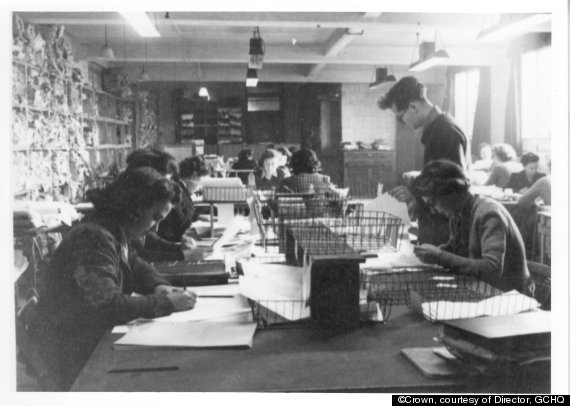
\includegraphics[width=0.5\textwidth]
    {figs/Bayes_figs/Women_in_Bletchley_Park.jpg}

    \caption{Women in Bletchley Park, (date of image: unknown); Source: \href{https://en.wikipedia.org/wiki/Women_in_Bletchley_Park}
    {Wikipedia}.}

    \label{fig:women-at-Bletchley}
\end{figure}


\subsubsection*{The problem: Naval Enigma and Bayesian hypothesis testing}

The Enigma machine encrypted each letter through a plugboard and a sequence of rotating wired rotors. For more informaiton, Alexander's post-war history and Mahon's \textit{History of Hut Eight} are excellent sources for Naval Enigma \cite{alexander1945,mahon1945}. Because the rotors moved as the machine was used, the substitution continually changed. Knowing how an Enigma machine worked was therefore not enough: the cryptanalysts had to infer its \textbf{unknown configuration} from intercepted messages and other evidence.

% \begin{figure}[H]
\begin{figure}[h]
\centering

% --- Enigma machine ---
\begin{minipage}[t]{0.42\textwidth}
    \centering

    \href{https://en.wikipedia.org/wiki/Cryptanalysis_of_the_Enigma\#/media/File:EnigmaMachineLabeled.jpg}{
        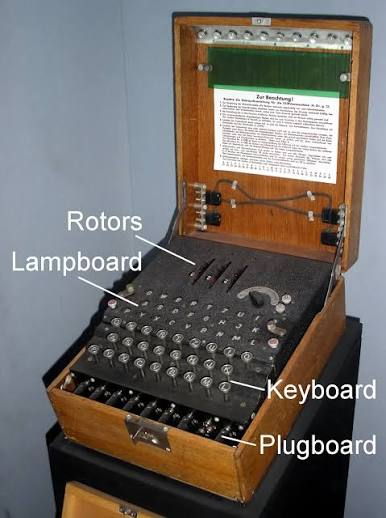
\includegraphics[height=7cm,keepaspectratio]
        {figs/Bayes_figs/Enigma.jpg}
    }

    \caption{A German Enigma machine.
    \href{https://en.wikipedia.org/wiki/Cryptanalysis_of_the_Enigma\#/media/File:EnigmaMachineLabeled.jpg}
    {Source: Wikipedia}.}

    \label{fig:enigma-machine}
\end{minipage}
\hspace{0.04\textwidth}
% --- Turing example ---
\begin{minipage}[t]{0.42\textwidth}
    \centering

    \href{https://arxiv.org/pdf/1505.04714}{
        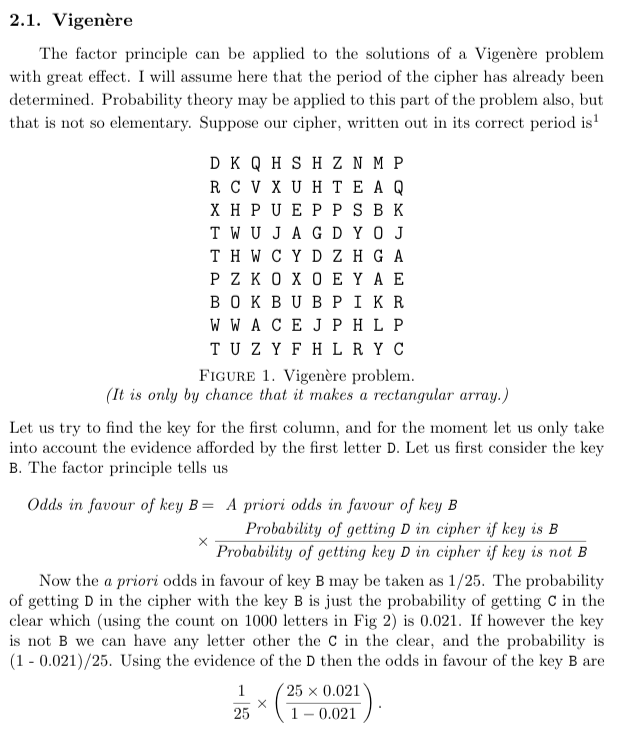
\includegraphics[height=7cm,keepaspectratio]
        {figs/Bayes_figs/Turing_Vigenere_example_bayesfactors.png}
    }

    \caption{Turing's Vigen\`ere cipher example in
    \textit{The Applications of Probability to Cryptography}.
    \href{https://arxiv.org/pdf/1505.04714}
    {Read the original text}.}

    \label{fig:turing-vigenere}
\end{minipage}

\end{figure}

For Naval Enigma, the difficulty could be formulated partly as a problem of \textbf{hypothesis testing}, more specifically \href{https://www.youtube.com/live/Ip8Ci5KUVRc?si=n0YSvhupRbd9GGuH}{Bayesian Hypothesis Testing}. Cryptanalysts compared pairs of intercepted messages by shifting one ciphertext relative to another. A proposed alignment represented a hypothesis that portions of the two messages had been enciphered at corresponding Enigma positions. If an alignment produced an unusually large number or pattern of letter coincidences, this provided evidence that the two portions were in \textit{depth} — that is, that corresponding letters had passed through the same sequence of Enigma substitutions. Probable depths could then be combined to infer relationships between message settings and to eliminate unlikely rotor orders, greatly reducing the subsequent search \cite{turing1941cryptography,alexander1945,zabell2012turing}.

Let $H_1$ and $H_0$ denote two competing hypotheses about the cipher
configuration, and let $E$ denote the observed evidence---for example, the pattern of coincidences produced by a particular message alignment. In odds form, Bayes' theorem gives

\begin{equation}
\boxed{
\underbrace{
\frac{P(H_1\mid E)}{P(H_0\mid E)}
}_{\text{posterior odds}}
=
\underbrace{
\frac{P(H_1)}{P(H_0)}
}_{\text{prior odds}}
\;
\underbrace{
\frac{P(E\mid H_1)}{P(E\mid H_0)}
}_{\substack{\text{Bayes factor}\\\text{(likelihood ratio)}}}
}
\end{equation}

Thus the \textbf{prior odds} are multiplied by a \textbf{likelihood ratio} \textit{measuring how strongly the observed evidence favours one hypothesis over the other}.  Turing described this idea in his wartime manuscript \textit{The Applications of Probability to Cryptography}, calling it the \emph{factor principle} \cite{turing1941cryptography,zabell2012turing}.

Because the calculations required the multiplication of many such factors, Turing expressed the resulting weight of evidence on a logarithmic scale using the \textbf{deciban} \cite{turing1941cryptography,good1979turing},

\begin{equation}
\boxed{
D
=
10\log_{10}
\left(
\frac{P(E\mid H_1)}{P(E\mid H_0)}
\right).
}
\end{equation}

Ten decibans multiplied the odds by $10$, while one deciban changed them by a factor of $10^{0.1}\approx1.26$. These ideas formed part of Turing's statistical procedure known as \emph{Banburismus}, which allowed the accumulation of evidence \textit{for or against candidate rotor relationships} and thereby eliminate unlikely rotor orders before committing scarce Bombe time \cite{good1979turing,alexander1945,zabell2012turing}.

The importance of \textbf{Turing's contribution} was therefore not the invention of Bayesian hypothesis testing itself, which had earlier roots in the work of Wrinch, Haldane and Jeffreys
\cite{wrinchjeffreys1919,wrinchjeffreys1921,
wrinchjeffreys1923,haldane1932,jeffreys1935,
etzwagenmakers2017}. His important contribution was to \textbf{make these ideas practical}. As new clues were obtained, the cryptanalysts could increase or decrease their confidence in different possible Enigma settings, gradually narrowing down the possibilities. Good later documented and further developed the wartime statistical ideas into the public literature here \cite{good1950,good1979turing}.

%% Final section ------------------------------------------


\subsection{The computational revolution in Bayesian inference: from Bayes’ theorem to algorithms (c. 1950–present)}
\label{sec:bayes-computational-history}

Post-1950 history of Bayesian statistics can be viewed as three connected developments:

\[
\boxed{
\begin{array}{lll}
\textbf{Computation} &:&
\text{how can difficult posterior distributions be calculated?}\\[1mm]
\textbf{Modelling} &:&
\text{what kinds of unknown objects can carry probability distributions?}\\[1mm]
\textbf{Learning and decisions} &:&
\text{how can uncertainty be used for prediction and action?}
\end{array}}
\]


%%%%%%%%%%%%%%%% Diagram 5 - split into 3 trees + COLOURRRR!! %%%%%%%%%%%%%%%%

\begin{figure}[H]
\centering

\begin{tikzpicture}[>=Latex]

\node[root] (root) at (0,0)
{Computational Bayesian inference};

% Main branches
\node[bluebranch]  (mcmc)   at (-5.1,-1.7) {MCMC};
\node[greenbranch] (filter) at (0.3,-1.7)  {Sequential inference};
\node[peachbranch] (approx) at (5.2,-1.7)  {Approximate inference};

\draw[arrow] (root) -- (mcmc);
\draw[arrow] (root) -- (filter);
\draw[arrow] (root) -- (approx);

% MCMC
\node[bluemethod] (metro) at (-5.1,-3.2)
{\textbf{Metropolis} (1953)};

\node[bluemethod] (mh) at (-5.1,-4.5)
{\textbf{Metropolis--Hastings} (1970)};

\node[bluemethod] (gibbs) at (-6.8,-5.9)
{\textbf{Gibbs sampling} (1984)};

\node[bluemethod] (hmc) at (-3.4,-5.9)
{\textbf{Hamiltonian MC} (1987)};

\draw[arrow] (mcmc) -- (metro);
\draw[arrow] (metro) -- (mh);
\draw[arrow] (mh) -- (gibbs);
\draw[arrow] (mh) -- (hmc);

% Sequential inference
\node[greenmethod] (kalman) at (0.5,-3.2)
{\textbf{Kalman filter} (1960)};

\node[greenmethod] (pf) at (0.5,-4.5)
{\textbf{Particle filter} (1993)};

\node[greenmethod] (pmcmc) at (0.5,-5.9)
{\textbf{Particle MCMC} (2010)};

\draw[arrow] (filter) -- (kalman);
\draw[arrow] (kalman) -- (pf);
\draw[arrow] (pf) -- (pmcmc);

% Approximate inference
\node[peachmethod] (vi) at (5.2,-3.2)
{\textbf{Variational inference} (1999)};

\draw[arrow] (approx) -- (vi);

\end{tikzpicture}

\caption{Selected developments in Bayesian computation after 1950.}
\label{fig:bayes-computation-tree}
\end{figure}


\begin{figure}[H]
\centering

\begin{tikzpicture}[
    >=Latex,
    root/.style={
        draw,
        rounded corners=3pt,
        fill=gray!20,
        font=\bfseries,
        align=center,
        text width=5.0cm,
        minimum height=0.9cm
    },
    branch/.style={
        draw,
        rounded corners=3pt,
        fill=gray!12,
        font=\bfseries,
        align=center,
        text width=3.6cm,
        minimum height=0.8cm
    },
    method/.style={
        draw,
        rounded corners=2pt,
        fill=gray!4,
        align=center,
        font=\small,
        text width=3.5cm,
        minimum height=0.72cm
    },
    arrow/.style={->, thick}
]

\node[root] (root) at (0,0)
{Bayesian modelling};

% THREE TYPES OF UNKNOWN OBJECT
\node[bluebranch] (parameters) at (-5.2,-1.7)
{Related parameters};

\node[greenbranch] (distributions) at (0,-1.7)
{Unknown distributions};

\node[peachbranch] (functions) at (5.2,-1.7)
{Unknown functions};

\draw[arrow] (root) -- (parameters);
\draw[arrow] (root) -- (distributions);
\draw[arrow] (root) -- (functions);

% RELATED PARAMETERS
\node[bluemethod] (emp) at (-5.2,-3.2)
{\textbf{Empirical Bayes} (1956)};

\node[bluemethod] (hier) at (-5.2,-4.6)
{\textbf{Hierarchical Bayes} (1972)};

\draw[arrow] (parameters) -- (emp);
\draw[arrow] (emp) -- (hier);

% UNKNOWN DISTRIBUTIONS
\node[greenmethod] (dp) at (0,-3.2)
{\textbf{Dirichlet process} (1973)};

\node[greenmethod] (dpm) at (0,-4.6)
{\textbf{DP mixtures} (1974)};

\node[greenmethod] (unknown) at (0,-6.0)
{\textbf{Unknown-component mixtures} (1997)};

\draw[arrow] (distributions) -- (dp);
\draw[arrow] (dp) -- (dpm);
\draw[arrow] (dpm) -- (unknown);

% FUNCTIONS
\node[peachmethod] (function) at (5.2,-3.2)
{\textbf{Bayesian function estimation} (1970)};

\node[peachmethod] (gp) at (5.2,-4.6)
{\textbf{Gaussian-process regression} (1978)};

\draw[arrow] (functions) -- (function);
\draw[arrow] (function) -- (gp);

\end{tikzpicture}

\caption{Selected developments in Bayesian modelling after 1950.
Bayesian uncertainty expanded from parameters to distributions and functions.}
\label{fig:bayes-modelling-tree}
\end{figure}




\begin{figure}[H]
\centering

\begin{tikzpicture}[>=Latex]

\node[root] (root) at (0,0)
{Bayesian learning and decision-making};

% Main branches
\node[bluebranch] (models) at (-5.1,-1.7)
{Probabilistic models};

\node[greenbranch] (optimisation) at (0,-1.7)
{Bayesian optimisation};

\node[peachbranch] (decisions) at (5.1,-1.7)
{Search and decisions};

\draw[arrow] (root) -- (models);
\draw[arrow] (root) -- (optimisation);
\draw[arrow] (root) -- (decisions);


% ------------------------------------------------------------
% Probabilistic models
% ------------------------------------------------------------

\node[bluemethod] (bn) at (-6.5,-3.3)
{\textbf{Bayesian networks}\\(1980s)};

\node[bluemethod] (bnn) at (-3.6,-3.3) %(-3.6,-3.2)
{\textbf{Bayesian neural networks}\\(1992)};

\node[bluemethod] (pgm) at (-6.5,-5.2)
{\textbf{Graphical models}\\(1990s)};

\node[bluemethod] (neal) at (-3.6,-5.2)
{\textbf{Neal's Bayesian NNs}\\(1996)};

\draw[arrow] (models) -- (bn);
\draw[arrow] (models) -- (bnn);

\draw[arrow] (bn) -- (pgm);
\draw[arrow] (bnn) -- (neal);


% ------------------------------------------------------------
% Bayesian optimisation
% ------------------------------------------------------------

\node[greenmethod] (kushner) at (0,-3.3)
{\textbf{Probabilistic optimisation}\\(1964)};

\node[greenmethod] (mockus) at (0,-5.2)
{\textbf{Bayesian global optimisation}\\(1970s)};

\node[greenmethod] (ego) at (0,-6.9)
{\textbf{EGO}\\(1998)};

\node[greenmethod] (ml) at (0,-8.6)
{\textbf{ML hyperparameters}\\(2012)};

\node[greenmethod] (alpha) at (0,-10.4)
{\textbf{AlphaGo tuning}\\(2016)};

\draw[arrow] (optimisation) -- (kushner);
\draw[arrow] (kushner) -- (mockus);
\draw[arrow] (mockus) -- (ego);
\draw[arrow] (ego) -- (ml);
\draw[arrow] (ml) -- (alpha);


% ------------------------------------------------------------
% Search / decisions
% ------------------------------------------------------------

\node[peachmethod] (central) at (5.1,-3.3)
{\textbf{SS Central America}\\(1980s)};

\node[peachmethod] (af) at (5.1,-5.2)
{\textbf{Air France AF447}\\(2011)};

\draw[arrow] (decisions) -- (central);
\draw[arrow] (central) -- (af);

\end{tikzpicture}

\caption{Selected developments and applications of Bayesian ideas in
machine learning and decision-making.}
\label{fig:bayes-learning-tree}
\end{figure}




%%%%%%%%%%%%%%%% Diagram 4 - split into 3 trees!! %%%%%%%%%%%%%%%%

\begin{figure}[H]
\centering

\begin{tikzpicture}[
    >=Latex,
    root/.style={
        draw,
        rounded corners=3pt,
        fill=gray!20,
        font=\bfseries,
        align=center,
        text width=5.2cm,
        minimum height=0.9cm
    },
    branch/.style={
        draw,
        rounded corners=3pt,
        fill=gray!12,
        font=\bfseries,
        align=center,
        text width=3.6cm,
        minimum height=0.8cm
    },
    method/.style={
        draw,
        rounded corners=2pt,
        fill=gray!4,
        align=center,
        font=\small,
        text width=3.3cm,
        minimum height=0.72cm
    },
    arrow/.style={->, thick}
]

% ROOT
\node[root] (root) at (0,0)
{Computational Bayesian inference};

% MAIN BRANCHES
\node[branch] (mcmc)   at (-5.2,-1.7) {MCMC};
\node[branch] (filter) at (0,-1.7)    {Sequential inference};
\node[branch] (approx) at (5.2,-1.7)  {Approximate inference};

\draw[arrow] (root) -- (mcmc);
\draw[arrow] (root) -- (filter);
\draw[arrow] (root) -- (approx);

% MCMC
\node[method] (metro) at (-5.2,-3.2)
{\textbf{Metropolis} (1953)};

\node[method] (mh) at (-5.2,-4.5)
{\textbf{Metropolis--Hastings} (1970)};

\node[method] (gibbs) at (-7.0,-5.9)
{\textbf{Gibbs sampling} (1984)};

\node[method] (hmc) at (-3.4,-5.9)
{\textbf{Hamiltonian MC} (1987)};

\draw[arrow] (mcmc) -- (metro);
\draw[arrow] (metro) -- (mh);
\draw[arrow] (mh) -- (gibbs);
\draw[arrow] (mh) -- (hmc);

% FILTERING
\node[method] (kalman) at (0,-3.2)
{\textbf{Kalman filter} (1960)};

\node[method] (pf) at (0,-4.5)
{\textbf{Particle filter} (1993)};

\node[method] (pmcmc) at (0,-5.9)
{\textbf{Particle MCMC} (2010)};

\draw[arrow] (filter) -- (kalman);
\draw[arrow] (kalman) -- (pf);
\draw[arrow] (pf) -- (pmcmc);

% VARIATIONAL
\node[method] (vi) at (5.2,-3.2)
{\textbf{Variational \newline inference} (1999)};

\draw[arrow] (approx) -- (vi);

\end{tikzpicture}

\caption{Selected developments in Bayesian computation after 1950.}
\label{fig:bayes-computation-tree}
\end{figure}




2. Bayesian modelling


\begin{figure}[H]
\centering

\begin{tikzpicture}[
    >=Latex,
    root/.style={
        draw,
        rounded corners=3pt,
        fill=gray!20,
        font=\bfseries,
        align=center,
        text width=5.0cm,
        minimum height=0.9cm
    },
    branch/.style={
        draw,
        rounded corners=3pt,
        fill=gray!12,
        font=\bfseries,
        align=center,
        text width=3.6cm,
        minimum height=0.8cm
    },
    method/.style={
        draw,
        rounded corners=2pt,
        fill=gray!4,
        align=center,
        font=\small,
        text width=3.5cm,
        minimum height=0.72cm
    },
    arrow/.style={->, thick}
]

\node[root] (root) at (0,0)
{Bayesian modelling};

% THREE TYPES OF UNKNOWN OBJECT
\node[branch] (parameters) at (-5.2,-1.7)
{Related parameters};

\node[branch] (distributions) at (0,-1.7)
{Unknown distributions};

\node[branch] (functions) at (5.2,-1.7)
{Unknown functions};

\draw[arrow] (root) -- (parameters);
\draw[arrow] (root) -- (distributions);
\draw[arrow] (root) -- (functions);

% RELATED PARAMETERS
\node[method] (emp) at (-5.2,-3.2)
{\textbf{Empirical Bayes} (1956)};

\node[method] (hier) at (-5.2,-4.6)
{\textbf{Hierarchical Bayes} (1972)};

\draw[arrow] (parameters) -- (emp);
\draw[arrow] (emp) -- (hier);

% UNKNOWN DISTRIBUTIONS
\node[method] (dp) at (0,-3.2)
{\textbf{Dirichlet process} (1973)};

\node[method] (dpm) at (0,-4.6)
{\textbf{DP mixtures} (1974)};

\node[method] (unknown) at (0,-6.0)
{\textbf{Unknown-component mixtures} (1997)};

\draw[arrow] (distributions) -- (dp);
\draw[arrow] (dp) -- (dpm);
\draw[arrow] (dpm) -- (unknown);

% FUNCTIONS
\node[method] (function) at (5.2,-3.2)
{\textbf{Bayesian function estimation} (1970)};

\node[method] (gp) at (5.2,-4.6)
{\textbf{Gaussian-process regression} (1978)};

\draw[arrow] (functions) -- (function);
\draw[arrow] (function) -- (gp);

\end{tikzpicture}

\caption{Selected developments in Bayesian modelling after 1950.
Bayesian uncertainty expanded from parameters to distributions and functions.}
\label{fig:bayes-modelling-tree}
\end{figure}



% I think this one is particularly nice because it shows the conceptual progression much better than a date-only timeline:

% [
% \boxed{\theta}
% \qquad
% \boxed{{\theta_i}}
% \qquad
% \boxed{F}
% \qquad
% \boxed{f(x)}.
% ]

So the reader immediately understands **what actually changed mathematically**.

And this gives you three women in historically meaningful places in the surrounding discussion:

* **Grace Wahba** — functions/splines/kernels;
* **Sylvia Richardson** — flexible mixture models;
* later applied hierarchical work including **Nicky Best**.

---

3. Bayesian learning, AI and decision-making
\begin{figure}[H]
\centering

\begin{tikzpicture}[
    >=Latex,
    root/.style={
        draw,
        rounded corners=3pt,
        fill=gray!20,
        font=\bfseries,
        align=center,
        text width=5.5cm,
        minimum height=0.9cm
    },
    branch/.style={
        draw,
        rounded corners=3pt,
        fill=gray!12,
        font=\bfseries,
        align=center,
        text width=3.6cm,
        minimum height=0.8cm
    },
    method/.style={
        draw,
        rounded corners=2pt,
        fill=gray!4,
        align=center,
        font=\small,
        text width=3.5cm,
        minimum height=0.72cm
    },
    arrow/.style={->, thick}
]

\node[root] (root) at (0,0)
{Bayesian learning and decision-making};

% MAIN BRANCHES
\node[branch] (models) at (-5.2,-1.7)
{Probabilistic models};

\node[branch] (optimisation) at (0,-1.7)
{Bayesian optimisation};

\node[branch] (decisions) at (5.2,-1.7)
{Search and decisions};

\draw[arrow] (root) -- (models);
\draw[arrow] (root) -- (optimisation);
\draw[arrow] (root) -- (decisions);

% PROBABILISTIC MODELS
\node[method] (bn) at (-6.2,-3.2)
{\textbf{Bayesian networks} (1980s)};

\node[method] (bnn) at (-4.2,-4.6)
{\textbf{Bayesian neural networks} (1992)};

\node[method] (pgm) at (-6.2,-4.6)
{\textbf{Graphical models} (1990s)};

\draw[arrow] (models) -- (bn);
\draw[arrow] (bn) -- (pgm);
\draw[arrow] (models) -- (bnn);

% BAYESIAN OPTIMISATION
\node[method] (kushner) at (0,-3.2)
{\textbf{Probabilistic optimisation} (1964)};

\node[method] (mockus) at (0,-4.5)
{\textbf{Bayesian global optimisation} (1970s)};

\node[method] (ego) at (0,-5.8)
{\textbf{EGO} (1998)};

\node[method] (ml) at (0,-7.1)
{\textbf{ML hyperparameters} (2012)};

\node[method] (alpha) at (0,-8.4)
{\textbf{AlphaGo tuning} (2016)};

\draw[arrow] (optimisation) -- (kushner);
\draw[arrow] (kushner) -- (mockus);
\draw[arrow] (mockus) -- (ego);
\draw[arrow] (ego) -- (ml);
\draw[arrow] (ml) -- (alpha);

% SEARCH
\node[method] (central) at (5.2,-3.2)
{\textbf{SS Central America} (1980s)};

\node[method] (af) at (5.2,-4.6)
{\textbf{Air France AF447} (2011)};

\draw[arrow] (decisions) -- (central);
\draw[arrow] (central) -- (af);

\end{tikzpicture}

\caption{Selected developments and applications of Bayesian ideas in
machine learning and decision-making.}
\label{fig:bayes-learning-tree}
\end{figure}




\newpage

%%%%%%%%%%%%%%%% Diagram 3 %%%%%%%%%%%%%%%%
\begin{landscape}

\begin{figure}[H]
\centering

{\Large\bfseries Bayesian inference after 1950}

\vspace{0.6cm}

% ============================================================
% COMMON TIKZ STYLE
% ============================================================

\tikzset{
    category/.style={
        draw,
        rounded corners=3pt,
        fill=gray!20,
        font=\bfseries,
        align=center,
        text width=5.2cm,
        minimum height=0.9cm
    },
    method/.style={
        draw,
        rounded corners=2pt,
        fill=gray!5,
        align=center,
        font=\small,
        text width=3.5cm,
        minimum height=0.75cm
    },
    arrow/.style={
        ->,
        >=Latex,
        thick
    }
}

% ============================================================
% COLUMN 1: COMPUTATION
% ============================================================

\begin{minipage}[t]{0.32\linewidth}
\centering

\begin{tikzpicture}

\node[category] (comp) at (0,0)
{Computational methods};

% --- MCMC branch ---
\node[method] (metro) at (-2.2,-1.6)
{\textbf{Metropolis}\\1953};

\node[method] (mh) at (-2.2,-3.0)
{\textbf{Metropolis--Hastings}\\1970};

\node[method] (gibbs) at (-3.5,-4.5)
{\textbf{Gibbs sampling}\\1984};

\node[method] (hmc) at (-0.9,-4.5)
{\textbf{Hamiltonian MC}\\1987};

\draw[arrow] (comp) -- (metro);
\draw[arrow] (metro) -- (mh);
\draw[arrow] (mh) -- (gibbs);
\draw[arrow] (mh) -- (hmc);

% --- Filtering branch ---
\node[method] (kalman) at (2.2,-1.6)
{\textbf{Kalman filter}\\1960};

\node[method] (pf) at (2.2,-3.0)
{\textbf{Particle filter}\\1993};

\node[method] (pmcmc) at (2.2,-4.5)
{\textbf{Particle MCMC}\\2010};

\draw[arrow] (comp) -- (kalman);
\draw[arrow] (kalman) -- (pf);
\draw[arrow] (pf) -- (pmcmc);

% --- VI ---
\node[method] (vi) at (0,-6.2)
{\textbf{Variational inference}\\1999};

\draw[arrow] (comp.south)
to[out=-90,in=90]
(vi.north);

\end{tikzpicture}

\end{minipage}
%
\hfill
%
% ============================================================
% COLUMN 2: MODELLING
% ============================================================

\begin{minipage}[t]{0.32\linewidth}
\centering

\begin{tikzpicture}

\node[category] (model) at (0,0)
{Bayesian modelling};

% --- Hierarchical ---
\node[method] (emp) at (-2.5,-1.6)
{\textbf{Empirical Bayes}\\1956};

\node[method] (hier) at (-2.5,-3.1)
{\textbf{Hierarchical Bayes}\\1972};

\draw[arrow] (model) -- (emp);
\draw[arrow] (emp) -- (hier);

% --- Functions / GP ---
\node[method] (func) at (0,-1.6)
{\textbf{Bayesian function estimation}\\1970};

\node[method] (gp) at (0,-3.1)
{\textbf{Gaussian-process regression}\\1978};

\draw[arrow] (model) -- (func);
\draw[arrow] (func) -- (gp);

% --- Nonparametrics ---
\node[method] (dp) at (2.5,-1.6)
{\textbf{Dirichlet process}\\1973};

\node[method] (dpm) at (2.5,-3.1)
{\textbf{DP mixtures}\\1974};

\node[method] (unknown) at (2.5,-4.7)
{\textbf{Unknown-dimensional mixtures}\\1997};

\draw[arrow] (model) -- (dp);
\draw[arrow] (dp) -- (dpm);
\draw[arrow] (dpm) -- (unknown);

\end{tikzpicture}

\end{minipage}
%
\hfill
%
% ============================================================
% COLUMN 3: LEARNING / AI
% ============================================================

\begin{minipage}[t]{0.32\linewidth}
\centering

\begin{tikzpicture}

\node[category] (learn) at (0,0)
{Learning, prediction\\and decision-making};

% --- Bayesian networks ---
\node[method] (bn) at (-2.3,-1.6)
{\textbf{Bayesian networks}\\1980s--1988};

\node[method] (pgm) at (-2.3,-3.1)
{\textbf{Graphical models}\\1990s--2000s};

\draw[arrow] (learn) -- (bn);
\draw[arrow] (bn) -- (pgm);

% --- Bayesian neural nets ---
\node[method] (bnn) at (2.3,-1.6)
{\textbf{Bayesian neural networks}\\1992};

\node[method] (neal) at (2.3,-3.1)
{\textbf{Neal's Bayesian NNs}\\1996};

\draw[arrow] (learn) -- (bnn);
\draw[arrow] (bnn) -- (neal);

% --- Bayesian optimisation ---
\node[method] (kushner) at (0,-4.8)
{\textbf{Probabilistic optimisation}\\Kushner, 1964};

\node[method] (mockus) at (0,-6.3)
{\textbf{Bayesian global optimisation}\\Mockus, 1970s};

\node[method] (ego) at (0,-7.8)
{\textbf{Efficient Global Optimisation}\\1998};

\node[method] (snoek) at (0,-9.3)
{\textbf{ML hyperparameter optimisation}\\2012};

\node[method] (alpha) at (0,-10.8)
{\textbf{AlphaGo tuning}\\2016};

\draw[arrow] (learn.south)
to[out=-90,in=90]
(kushner.north);

\draw[arrow] (kushner) -- (mockus);
\draw[arrow] (mockus) -- (ego);
\draw[arrow] (ego) -- (snoek);
\draw[arrow] (snoek) -- (alpha);

\end{tikzpicture}

\end{minipage}

\vspace{0.6cm}

{\small
\textit{Important later connections:}
Particle MCMC combines ideas from MCMC and particle filtering;
Gaussian processes became important surrogate models in Bayesian optimisation;
and both MCMC and variational inference are used for inference in Bayesian
neural networks.
}

\caption{A simplified genealogy of selected developments in Bayesian
statistics after 1950. The diagram separates developments in computation,
modelling, and learning and decision-making.}

\label{fig:bayesian-post1950-tree}

\end{figure}

\end{landscape}

%%%%%%%%%%%%%%%% Diagram 2 %%%%%%%%%%%%%%%%

\begin{landscape}

\begin{figure}[H]
\centering

\begin{tikzpicture}[
    >=Latex,
    root/.style={
        draw,
        rounded corners=3pt,
        fill=gray!20,
        font=\bfseries,
        align=center,
        text width=4.2cm,
        minimum height=0.8cm
    },
    category/.style={
        draw,
        rounded corners=3pt,
        fill=gray!15,
        font=\bfseries,
        align=center,
        text width=3.6cm,
        minimum height=0.75cm
    },
    method/.style={
        draw,
        rounded corners=2pt,
        fill=gray!5,
        align=center,
        font=\small,
        text width=2.8cm,
        minimum height=0.7cm
    },
    direct/.style={
        ->,
        thick
    },
    influence/.style={
        ->,
        dashed,
        thick,
        gray
    }
]

% ============================================================
% ROOT
% ============================================================

\node[root] (root) at (0,0)
{Bayesian inference after 1950};

% ============================================================
% THREE MAIN BRANCHES
% ============================================================

\node[category] (comp)  at (-7,-1.6)
{Computational methods};

\node[category] (model) at (0,-1.6)
{Bayesian modelling};

\node[category] (learn) at (7,-1.6)
{Learning, prediction\\and decision-making};

\draw[direct] (root) -- (comp);
\draw[direct] (root) -- (model);
\draw[direct] (root) -- (learn);


% ============================================================
% COMPUTATION
% ============================================================

% MCMC branch
\node[method] (metro) at (-9,-3.3)
{\textbf{Metropolis}\\1953};

\node[method] (mh) at (-9,-4.6)
{\textbf{Metropolis--Hastings}\\1970};

\node[method] (gibbs) at (-10.6,-6.0)
{\textbf{Gibbs sampling}\\1984};

\node[method] (hmc) at (-7.4,-6.0)
{\textbf{Hamiltonian MC}\\1987};

\draw[direct] (comp) -- (metro);
\draw[direct] (metro) -- (mh);
\draw[direct] (mh) -- (gibbs);
\draw[direct] (mh) -- (hmc);


% Filtering branch
\node[method] (kalman) at (-5,-3.3)
{\textbf{Kalman filter}\\1960};

\node[method] (pf) at (-5,-4.6)
{\textbf{Particle filter}\\1993};

\node[method] (pmcmc) at (-5,-6.0)
{\textbf{Particle MCMC}\\2010};

\draw[direct] (comp) -- (kalman);
\draw[direct] (kalman) -- (pf);
\draw[direct] (pf) -- (pmcmc);

% MCMC contributes to PMCMC
\draw[influence]
(mh.east) to[bend left=10] (pmcmc.west);


% VI
\node[method] (vi) at (-7,-7.6)
{\textbf{Variational inference}\\1999};

\draw[direct]
(comp.south) to[out=-90,in=90] (vi.north);


% ============================================================
% MODELLING
% ============================================================

% Hierarchical branch
\node[method] (emp) at (-2.4,-3.3)
{\textbf{Empirical Bayes}\\1956};

\node[method] (hier) at (-2.4,-4.7)
{\textbf{Hierarchical Bayes}\\1972};

\draw[direct] (model) -- (emp);
\draw[direct] (emp) -- (hier);


% Function / GP branch
\node[method] (func) at (0.8,-3.3)
{\textbf{Bayesian function estimation}\\1970};

\node[method] (gp) at (0.8,-4.7)
{\textbf{Gaussian-process regression}\\1978};

\draw[direct] (model) -- (func);
\draw[direct] (func) -- (gp);


% Nonparametrics branch
\node[method] (dp) at (4,-3.3)
{\textbf{Dirichlet process}\\1973};

\node[method] (dpm) at (4,-4.7)
{\textbf{DP mixtures}\\1974};

\node[method] (rj) at (4,-6.1)
{\textbf{Unknown-dimensional mixtures}\\1997};

\draw[direct] (model) -- (dp);
\draw[direct] (dp) -- (dpm);
\draw[direct] (dpm) -- (rj);


% ============================================================
% LEARNING / AI
% ============================================================

% Bayesian networks
\node[method] (bn) at (7,-3.3)
{\textbf{Bayesian networks}\\1980s--1988};

\node[method] (pgm) at (7,-4.7)
{\textbf{Graphical models}\\1990s--2000s};

\draw[direct] (learn) -- (bn);
\draw[direct] (bn) -- (pgm);


% Bayesian neural networks
\node[method] (bnn) at (10.2,-3.3)
{\textbf{Bayesian neural networks}\\1992};

\node[method] (neal) at (10.2,-4.7)
{\textbf{Neal's Bayesian NNs}\\1996};

\draw[direct] (learn) -- (bnn);
\draw[direct] (bnn) -- (neal);


% Bayesian optimisation -- use vertical space
\node[method] (kushner) at (7,-6.5)
{\textbf{Stochastic optimisation}\\1964};

\node[method] (mockus) at (7,-7.9)
{\textbf{Bayesian global optimisation}\\1970s};

\node[method] (ego) at (7,-9.3)
{\textbf{Efficient Global Optimisation}\\1998};

\node[method] (snoek) at (7,-10.7)
{\textbf{ML hyperparameter optimisation}\\2012};

\node[method] (alphago) at (7,-12.1)
{\textbf{AlphaGo tuning}\\2016};

\draw[direct]
(learn.south) to[out=-90,in=90] (kushner.north);

\draw[direct] (kushner) -- (mockus);
\draw[direct] (mockus) -- (ego);
\draw[direct] (ego) -- (snoek);
\draw[direct] (snoek) -- (alphago);


% ============================================================
% CROSS-CONNECTIONS
% ============================================================

% GP -> Bayesian optimisation
\draw[influence]
(gp.east)
to[bend left=15]
node[midway, above, sloped, font=\scriptsize]
{GP surrogate}
(ego.west);

% MCMC -> Bayesian neural networks
\draw[influence]
(hmc.east)
to[bend right=12]
(bnn.west);

% VI -> Bayesian neural networks
\draw[influence]
(vi.east)
to[bend right=12]
(bnn.south west);


% ============================================================
% LEGEND
% ============================================================

\node[align=left,font=\scriptsize] at (0,-12.2)
{
\tikz{\draw[direct] (0,0)--(0.8,0);}
\; methodological development
\qquad\qquad
\tikz{\draw[influence] (0,0)--(0.8,0);}
\; later connection / influence
};

\end{tikzpicture}

\caption{A simplified genealogy of selected developments in Bayesian statistics
after 1950. Solid arrows indicate a broadly direct methodological development;
dashed arrows indicate important later connections rather than a claim of
direct historical descent.}

\label{fig:bayesian-post1950-tree}

\end{figure}

\end{landscape}


%%%%%%%%%%%%%%%% Diagram 1 %%%%%%%%%%%%%%%%
\begin{landscape}

\begin{figure}[H]
\centering


\begin{tikzpicture}[
    scale=0.5,
    transform shape,
    node distance=0.65cm and 0.8cm,
    >=Latex,
    root/.style={
        draw,
        rounded corners=3pt,
        fill=gray!20,
        font=\bfseries,
        align=center,
        minimum width=5.5cm,
        minimum height=0.9cm
    },
    category/.style={
        draw,
        rounded corners=3pt,
        fill=gray!15,
        font=\bfseries,
        align=center,
        text width=4.6cm,
        minimum height=0.85cm
    },
    method/.style={
        draw,
        rounded corners=2pt,
        fill=gray!5,
        align=center,
        font=\small,
        text width=3.5cm,
        minimum height=0.75cm
    },
    direct/.style={
        ->,
        thick
    },
    influence/.style={
        ->,
        dashed,
        thick,
        gray
    }
]

% ============================================================
% ROOT
% ============================================================

\node[root] (root)
{\textbf{Bayesian inference after 1950}};

% Main categories
\node[category, below left=1.2cm and 5.6cm of root] (comp)
{Computational methods};

\node[category, below=1.2cm of root] (model)
{Bayesian modelling};

\node[category, below right=1.2cm and 5.6cm of root] (learn)
{Learning, prediction\\and decision-making};

\draw[direct] (root) -- (comp);
\draw[direct] (root) -- (model);
\draw[direct] (root) -- (learn);


% ============================================================
% COMPUTATIONAL BRANCH
% ============================================================

\node[method, below left=0.9cm and 1.5cm of comp] (metro)
{\textbf{Metropolis}\\1953};

\node[method, below=0.7cm of metro] (mh)
{\textbf{Metropolis--Hastings}\\1970};

\node[method, below left=0.7cm and 0.15cm of mh] (gibbs)
{\textbf{Gibbs sampling}\\1984};

\node[method, below right=0.7cm and 0.15cm of mh] (hmc)
{\textbf{Hamiltonian MC}\\1987};

\draw[direct] (comp) -- (metro);
\draw[direct] (metro) -- (mh);
\draw[direct] (mh) -- (gibbs);
\draw[direct] (mh) -- (hmc);


% Sequential filtering branch

\node[method, below right=0.9cm and 1.5cm of comp] (kalman)
{\textbf{Kalman filter}\\1960};

\node[method, below=0.7cm of kalman] (pf)
{\textbf{Particle filter}\\1993};

\node[method, below=0.7cm of pf] (pmcmc)
{\textbf{Particle MCMC}\\2010};

\draw[direct] (comp) -- (kalman);
\draw[direct] (kalman) -- (pf);
\draw[direct] (pf) -- (pmcmc);

% MCMC also feeds into Particle MCMC
\draw[influence] (mh.east) to[bend left=15] (pmcmc.west);


% Variational inference
\node[method, below=5.2cm of comp] (vi)
{\textbf{Variational inference}\\1999};

\draw[direct] (comp.south) to[out=-90,in=90] (vi.north);


% ============================================================
% MODELLING BRANCH
% ============================================================

% Empirical / hierarchical
\node[method, below left=0.9cm and 1.5cm of model] (emp)
{\textbf{Empirical Bayes}\\1956};

\node[method, below=0.7cm of emp] (hier)
{\textbf{Hierarchical Bayes}\\1972};

\draw[direct] (model) -- (emp);
\draw[direct] (emp) -- (hier);


% Functions / Gaussian processes
\node[method, below=0.9cm of model] (wahba)
{\textbf{Bayesian function estimation}\\1970};

\node[method, below=0.7cm of wahba] (gp)
{\textbf{Bayesian GP regression}\\1978};

\draw[direct] (model) -- (wahba);
\draw[direct] (wahba) -- (gp);


% Bayesian nonparametrics
\node[method, below right=0.9cm and 1.5cm of model] (dp)
{\textbf{Dirichlet process}\\1973};

\node[method, below=0.7cm of dp] (dpm)
{\textbf{DP mixtures}\\1974};

\node[method, below=0.7cm of dpm] (rj)
{\textbf{Unknown-dimensional mixtures}\\1997};

\draw[direct] (model) -- (dp);
\draw[direct] (dp) -- (dpm);
\draw[direct] (dpm) -- (rj);


% ============================================================
% LEARNING / AI BRANCH
% ============================================================

% Bayesian networks
\node[method, below left=0.9cm and 1.7cm of learn] (bn)
{\textbf{Bayesian networks}\\1980s--1988};

\node[method, below=0.7cm of bn] (pgm)
{\textbf{Probabilistic graphical models}\\1990s--2000s};

\draw[direct] (learn) -- (bn);
\draw[direct] (bn) -- (pgm);


% Bayesian neural networks
\node[method, below=0.9cm of learn] (bnn)
{\textbf{Bayesian neural networks}\\1992};

\node[method, below=0.7cm of bnn] (neal)
{\textbf{Neal's Bayesian NNs}\\1996};

\draw[direct] (learn) -- (bnn);
\draw[direct] (bnn) -- (neal);


% Bayesian optimisation
\node[method, below right=0.9cm and 1.7cm of learn] (kushner)
{\textbf{Stochastic optimisation}\\Kushner, 1964};

\node[method, below=0.7cm of kushner] (mockus)
{\textbf{Bayesian global optimisation}\\1970s};

\node[method, below=0.7cm of mockus] (ego)
{\textbf{Efficient Global Optimisation}\\1998};

\node[method, below=0.7cm of ego] (snoek)
{\textbf{ML hyperparameter optimisation}\\2012};

\node[method, below=0.7cm of snoek] (alphago)
{\textbf{AlphaGo tuning}\\2016};

\draw[direct] (learn) -- (kushner);
\draw[direct] (kushner) -- (mockus);
\draw[direct] (mockus) -- (ego);
\draw[direct] (ego) -- (snoek);
\draw[direct] (snoek) -- (alphago);


% ============================================================
% CROSS-BRANCH CONNECTIONS
% ============================================================

% Gaussian processes feed Bayesian optimisation
\draw[influence]
    (gp.east)
    to[bend left=12]
    node[midway, above, sloped, font=\scriptsize]
    {GP surrogate models}
    (ego.west);

% MCMC / VI enable Bayesian neural networks
\draw[influence]
    (hmc.east)
    to[bend right=15]
    (bnn.west);

\draw[influence]
    (vi.east)
    to[bend right=12]
    (bnn.south west);


% ============================================================
% LEGEND
% ============================================================

\node[
    align=left,
    font=\scriptsize,
    below=0.8cm of vi,
    xshift=6.0cm
] (legend)
{
\tikz{\draw[direct] (0,0)--(0.8,0);}
\; methodological development
\qquad
\tikz{\draw[influence] (0,0)--(0.8,0);}
\; later connection / influence
};

\end{tikzpicture}

\caption{A simplified genealogy of selected developments in Bayesian
statistics after 1950. Solid arrows indicate a broadly direct methodological
development; dashed arrows indicate important later connections rather than
a claim of direct historical descent.}

\label{fig:bayesian-post1950-tree}
\end{figure}

\end{landscape}




%%%%%%%%%% -- tha three tables 
\newpage

% Add to the preamble if not already included:
% \usepackage{booktabs}
% \usepackage{tabularx}
% \usepackage{array}

\subsection{Bayesian inference after 1950: computation, modelling and machine learning
(c.~1950--present)}
\label{sec:bayes-post1950}

By the middle of the twentieth century, the central principle of Bayesian
inference was already well established. The developments that followed can be
viewed through three closely connected histories: new methods for
\textbf{computing} difficult posterior distributions, new ways of
\textbf{modelling} increasingly complicated unknown objects, and the spread of
Bayesian ideas into \textbf{machine learning and decision-making}.

% ============================================================
\subsubsection{The computational revolution}

\begin{table}[H]
\centering
\small
\renewcommand{\arraystretch}{1.25}
\begin{tabularx}{\textwidth}{
>{\raggedright\arraybackslash}p{0.20\textwidth}
>{\raggedright\arraybackslash}p{0.34\textwidth}
>{\raggedright\arraybackslash}X}
\toprule
\textbf{Method} &
\textbf{Historical development} &
\textbf{Problem being addressed} \\
\midrule

\textbf{Metropolis algorithm}
&
\textbf{1953}: Nicholas Metropolis, \textbf{Arianna Rosenbluth},
Marshall Rosenbluth, \textbf{Augusta Teller} and Edward Teller developed a
Monte Carlo method on the MANIAC computer at Los Alamos
\cite{metropolis1953}. Arianna Rosenbluth played an important role in its
implementation \cite{gubernatis2005}.
&
Originally developed for statistical physics: how can a computer generate
samples from a complicated probability distribution when direct calculation
is impractical? \\

\textbf{Kalman filter}
&
\textbf{1960}: Rudolf Kalman introduced recursive filtering and prediction
methods in control theory \cite{kalman1960}.
&
How can the unknown state of a changing system be continually estimated as
new, noisy observations arrive? For linear-Gaussian models this is equivalent
to exact sequential Bayesian updating. \\

\textbf{Metropolis--Hastings}
&
\textbf{1970}: W.~K. Hastings generalised the 1953 Metropolis method
\cite{hastings1970}.
&
How can complicated target distributions---later especially Bayesian
posteriors---be explored by simulation without evaluating difficult
normalising integrals? \\

\textbf{Gibbs sampling}
&
\textbf{1984}: Stuart and Donald Geman used Gibbs sampling in Bayesian image
restoration \cite{geman1984}. Gelfand and Smith later helped establish such
sampling methods as general tools for Bayesian inference
\cite{gelfandsmith1990}.
&
How can a complicated multivariate distribution be sampled by repeatedly
sampling from simpler conditional distributions? \\

\textbf{Hamiltonian Monte Carlo}
&
\textbf{1987}: Duane, Kennedy, Pendleton and Roweth introduced
\emph{Hybrid Monte Carlo} in lattice field theory \cite{duane1987}.
&
How can simulation move more efficiently through high-dimensional probability
distributions than a simple random-walk MCMC algorithm? \\

\textbf{Particle filter}
&
\textbf{1993}: Neil Gordon, David Salmond and Adrian Smith introduced the
bootstrap particle filter for nonlinear and non-Gaussian Bayesian state
estimation \cite{gordon1993}.
&
How can sequential Bayesian updating be performed when the assumptions needed
for an exact Kalman filter no longer hold? The posterior is represented by
many simulated ``particles''. \\

\textbf{Variational inference}
&
\textbf{1999}: Michael Jordan, Zoubin Ghahramani, Tommi Jaakkola and Lawrence
Saul gave an influential treatment of variational methods for graphical
models \cite{jordan1999}.
&
Can a difficult posterior be approximated by a simpler distribution found
through optimisation rather than by repeated random sampling? \\

\textbf{Particle MCMC}
&
\textbf{2010}: Christophe Andrieu, Arnaud Doucet and Roman Holenstein combined
particle filtering with MCMC \cite{andrieu2010}.
&
How can Bayesian inference be performed jointly over unknown parameters and
hidden state trajectories in difficult nonlinear state-space models? \\

\textbf{BUGS and probabilistic programming}
&
The BUGS project at the MRC Biostatistics Unit, with later important
contributions from statisticians including \textbf{Nicky Best}, made
Gibbs-sampling-based Bayesian modelling widely accessible
\cite{lunn2009}. Later systems such as Stan continued this approach.
&
How can researchers specify complicated Bayesian models without having to
derive and program a new sampling algorithm for every problem? \\

\bottomrule
\end{tabularx}
\caption{Selected milestones in the computational development of Bayesian
inference after 1950. Several important methods originated in physics,
engineering or computer science before being adopted for Bayesian computation.}
\label{tab:bayes-computation-timeline}
\end{table}


% ============================================================
\subsubsection{The modelling revolution}

\begin{table}[H]
\centering
\small
\renewcommand{\arraystretch}{1.25}
\begin{tabularx}{\textwidth}{
>{\raggedright\arraybackslash}p{0.20\textwidth}
>{\raggedright\arraybackslash}p{0.34\textwidth}
>{\raggedright\arraybackslash}X}
\toprule
\textbf{Method} &
\textbf{Historical development} &
\textbf{Problem being addressed} \\
\midrule

\textbf{Empirical Bayes}
&
\textbf{1956}: Herbert Robbins proposed an ``empirical Bayes'' approach in
which information from many related observations could help determine the
distribution governing their parameters \cite{robbins1956}.
&
Must a prior distribution always be specified completely in advance, or can
information across a population of related observations help estimate it? \\

\textbf{Bayesian estimation of functions}
&
\textbf{1970}: George Kimeldorf and \textbf{Grace Wahba} established a
correspondence between Bayesian estimation of stochastic processes and
smoothing by splines \cite{kimeldorfwahba1970}.
&
How can uncertainty be placed not merely on a finite number of parameters but
on an entire unknown function? This work also helped connect Bayesian
estimation with smoothing and later kernel methods. \\

\textbf{Hierarchical Bayes}
&
\textbf{1972}: Dennis Lindley and Adrian Smith developed influential
hierarchical prior structures for linear models \cite{lindleysmith1972}.
&
How can related groups---for example hospitals, schools or regions---share
information without assuming that they are identical? Hierarchical models
provide the basis for \emph{partial pooling}. \\

\textbf{Bayesian nonparametrics}
&
\textbf{1973}: Thomas Ferguson introduced the \textbf{Dirichlet process}
as a prior distribution over probability distributions
\cite{ferguson1973}.
&
How can the unknown object itself be an entire probability distribution rather
than a parameter vector of fixed dimension? \\

\textbf{Dirichlet-process mixtures}
&
\textbf{1974}: Charles Antoniak developed mixtures of Dirichlet processes
\cite{antoniak1974}.
&
How can flexible mixture and clustering models be constructed without fixing
all of their complexity in advance? \\

\textbf{Gaussian-process regression}
&
\textbf{1978}: Anthony O'Hagan developed an explicitly Bayesian approach to
flexible curve fitting and prediction \cite{ohagan1978}.
&
How can probability distributions be placed directly over possible functions,
allowing predictions to include uncertainty about the shape of the function
itself? Gaussian processes later became closely connected with kernel methods. \\

\textbf{Unknown-dimensional mixture models}
&
\textbf{1997}: \textbf{Sylvia Richardson} and Peter Green developed Bayesian
mixture modelling with an unknown number of components using reversible-jump
MCMC \cite{richardsongreen1997}.
&
What if even the number of components or effective parameters in a model is
unknown and must itself be inferred from the data? \\

\bottomrule
\end{tabularx}
\caption{Selected developments in Bayesian modelling. The historical progression
extended Bayesian uncertainty from individual parameters to hierarchies,
probability distributions and entire functions.}
\label{tab:bayes-modelling-timeline}
\end{table}


% ============================================================
\subsubsection{Bayesian learning, prediction and decision-making}

\begin{table}[H]
\centering
\small
\renewcommand{\arraystretch}{1.25}
\begin{tabularx}{\textwidth}{
>{\raggedright\arraybackslash}p{0.20\textwidth}
>{\raggedright\arraybackslash}p{0.34\textwidth}
>{\raggedright\arraybackslash}X}
\toprule
\textbf{Method / application} &
\textbf{Historical development} &
\textbf{Problem being addressed} \\
\midrule

\textbf{Bayesian optimisation}
&
\textbf{1964}: Harold Kushner developed an early probabilistic method for
locating the maximum of an expensive noisy function \cite{kushner1964}.
Jonas Mockus developed explicitly Bayesian global-optimisation methods during
the 1970s.
&
If evaluating a function is very expensive, how can uncertainty about its
unknown shape be used to decide where the next evaluation should be made? \\

\textbf{Bayesian networks}
&
During the \textbf{1980s}, Judea Pearl developed probabilistic graphical
methods for reasoning under uncertainty, culminating in his 1988 book
\emph{Probabilistic Reasoning in Intelligent Systems} \cite{pearl1988}.
Lauritzen and Spiegelhalter also developed efficient local probability
calculations for graphical models in 1988
\cite{lauritzenspiegelhalter1988}.
&
How can a very large joint probability distribution be represented and
computed efficiently by exploiting conditional independence between
variables? \\

\textbf{Bayesian search theory}
&
Lawrence Stone described the successful probabilistic search for the wreck of
the \textit{SS Central America} in 1992 \cite{stone1992}. Later, Stone,
\textbf{Colleen Keller}, Thomas Kratzke and Johan Strumpfer used Bayesian
search ideas in the search for Air France Flight AF447
\cite{stone2014}.
&
How should limited search resources be allocated when the location of a target
is uncertain and evidence from unsuccessful searches continually changes that
uncertainty? \\

\textbf{Bayesian neural networks}
&
\textbf{1992}: David MacKay developed a practical Bayesian framework for
backpropagation networks \cite{mackay1992}. Radford Neal extended Bayesian
neural-network methods during the 1990s \cite{neal1996}.
&
Instead of learning one ``best'' set of neural-network weights, can uncertainty
about the weights themselves be represented and propagated into predictions? \\

\textbf{Efficient Global Optimisation}
&
\textbf{1998}: Jones, Schonlau and Welch developed the influential
\emph{Efficient Global Optimization} approach \cite{jones1998}.
&
How can a probabilistic surrogate, often a Gaussian process, balance exploring
uncertain regions with exploiting regions already believed to contain good
solutions? \\

\textbf{Probabilistic graphical models}
&
Later researchers including \textbf{Daphne Koller} helped connect Bayesian
networks and related graphical models with modern machine learning; her
influential text with Nir Friedman systematised this field
\cite{kollerfriedman2009}.
&
How can complex probabilistic models support both automated inference and
learning from large datasets? \\

\textbf{Bayesian optimisation in machine learning}
&
\textbf{2012}: Snoek, Larochelle and Adams demonstrated Bayesian optimisation
for machine-learning hyperparameter selection \cite{snoek2012}.
DeepMind later reported using Bayesian optimisation to tune
\textbf{AlphaGo} \cite{chen2018}.
&
Training modern machine-learning systems can be extremely expensive. How can
researchers decide which hyperparameter settings are worth testing without
exhaustively trying every possibility? \\

\bottomrule
\end{tabularx}
\caption{Selected developments in the spread of Bayesian ideas into artificial
intelligence, machine learning and decision-making.}
\label{tab:bayes-learning-timeline}
\end{table}


\medskip

Taken together, the three timelines show that the post-1950 development of
Bayesian statistics was not a single sequence of new versions of Bayes'
theorem. Instead, Bayesian ideas expanded in three directions:
\textbf{new algorithms made inference computable, new models enlarged what
could be treated as uncertain, and new applications used that uncertainty for
prediction and decision-making.}
```



\section{Conslusions}
% \paragraph{Bayes and human reasoning.}

From Bayes and Laplace to modern computation and machine learning, Bayesian inference has developed into a general framework for \textbf{learning from evidence under uncertainty}.

Bayesian ideas have also returned to a much older question: \emph{how do humans reason under uncertainty?} The psychologist \textbf{Daniel Kahneman} (1934--2024), whose work with Amos Tversky transformed the study of judgement and decision-making, explicitly describes Bayes' rule as the normative rule for combining prior beliefs with the diagnosticity of new evidence, while noting that \textit{intuitive judgement} often fails to do this correctly \cite[p.~154]{kahneman2011}.

More recently, the psychologist and neuroscientist \textbf{Lisa Feldman Barrett} (b.~1963) has connected Bayesian ideas with theories of perception and learning. Barrett describes the brain as a predictive system that uses past experience to form hypotheses about incoming sensory information and revises those predictions in light of new evidence \cite{barrett2017}. In the scientific notes accompanying \emph{How Emotions Are Made}, she explicitly connects this predictive-coding framework with Bayes' theorem and Bayesian inference. 

Thus, Bayesian reasoning returns to its original problem: \textbf{How should we change what we believe when new evidence arrives?}












%% Final sectin drafts - old ------------------------------------------

% add: The Sequential Test \& Wald ConnectionTuring's use of accumulated decibans to reach a decision threshold (stopping rule when $W > \text{threshold}$) is effectively Abraham Wald’s Sequential Probability Ratio Test (SPRT), developed independently in the US around the same time.

\subsection{The computational revolution in Bayesian inference: from Bayes’ theorem to algorithms (c. 1950–present)}
\label{sec:bayes-computational-history}


MCMC
Particle filters
There is also a different but related path/genealogical degeneracy problem: repeated resampling means particles that look different today can all share only a few ancestors, making inference about earlier states—the smoothing problem—difficult. Reviews of modern filtering explicitly identify high-dimensional state estimation and inference over state histories as major challenges

particle MCMC. Andrieu, Doucet and Holenstein in 2010 combined the two branches of your story: particle filters are placed inside MCMC methods, making joint Bayesian inference over unknown parameters and hidden states possible for difficult nonlinear state-space models.
Air France AF447; SS Central America (ship of gold)

Variational Inference --> optimisation problem
This became especially influential in machine learning because optimisation can often be considerably faster than traditional MCMC on very large problems, although the posterior approximation introduces another source of error. Jordan, Ghahramani, Jaakkola and Saul gave an influential treatment of variational methods for graphical models around 1999; the later Blei–Kucukelbir–McAuliffe review explicitly describes VI as optimisation-based approximate Bayesian inference

AlphaGo
It has a much older history than DeepMind. Kushner developed an early stochastic-process approach to expensive optimisation in 1964; Mockus developed Bayesian global-optimisation methods in the 1970s; Jones, Schonlau and Welch's 1998 Efficient Global Optimization paper became another major milestone; and Bayesian optimisation became particularly important for machine-learning hyperparameters in work such as Snoek, Larochelle and Adams in 2012

Slightly different to mathematics:
neuroscientist Lisa Feldman Barrett \& psychologist Daniel Kahneman's view of the human learning and reasoning is also modelled by a bayesian framework

\newpage

%%%%%%%%%%%%%%%5 version 2- 3 pages
\subsection{V3 3 pages The computational and modelling revolution in Bayesian inference
(c.~1950--present)}
\label{sec:bayes-post1950}

By the middle of the twentieth century, the central principle of Bayesian
inference was already well established. The major developments that followed
were therefore less about changing Bayes' theorem itself than about making it
\textbf{computable}, extending the kinds of objects that could be
\textbf{modelled}, and applying Bayesian reasoning to increasingly complex
problems in science and machine learning.

% ============================================================
\subsubsection{The computational revolution}

For much of its earlier history, Bayesian inference was practical only when
the required posterior distributions and integrals could be calculated
analytically. Electronic computers changed this dramatically. One of the
most important developments originated in mathematical physics rather than
statistics. In 1953 Nicholas Metropolis, \textbf{Arianna Rosenbluth},
Marshall Rosenbluth, \textbf{Augusta Teller} and Edward Teller introduced a
Monte Carlo method for sampling from complicated probability distributions
using the MANIAC computer at Los Alamos \cite{metropolis1953}. Arianna
Rosenbluth was closely involved in implementing the algorithm, although the
method subsequently became known simply as the ``Metropolis algorithm''
\cite{gubernatis2005}. W.~K. Hastings generalised it in 1970
\cite{hastings1970}, producing the \textbf{Metropolis--Hastings algorithm}.
These methods became fundamental to Bayesian statistics because a difficult
posterior distribution could now be explored by simulation rather than
calculated exactly.

The broader family became known as \textbf{Markov chain Monte Carlo (MCMC)}.
Further developments included Gibbs sampling, used by Geman and Geman in
Bayesian image restoration in 1984 \cite{geman1984}, and Hamiltonian Monte
Carlo, introduced by Duane et al.\ in 1987 in lattice field theory
\cite{duane1987}. Gelfand and Smith's influential 1990 paper helped establish
MCMC as a general method for Bayesian statistical computation
\cite{gelfandsmith1990}. Software subsequently made these methods accessible
to a much wider community. The \textbf{BUGS} project---\emph{Bayesian
inference Using Gibbs Sampling}---and later systems such as Stan allowed
researchers to specify complicated probability models without constructing
each sampling procedure from scratch \cite{lunn2009}. Statistician
\textbf{Nicky Best} was among the important contributors to the development
and dissemination of WinBUGS and applied Bayesian modelling.

A second computational branch concerned quantities that change through time.
Kalman's 1960 filtering method arose in engineering and control theory
\cite{kalman1960}, but for linear-Gaussian models it can be interpreted as
exact sequential Bayesian updating. Gordon, Salmond and Smith extended this
idea to nonlinear and non-Gaussian systems with their influential 1993
\textbf{particle filter} \cite{gordon1993}. Here a probability distribution
is represented by many simulated ``particles'', which are repeatedly
propagated, weighted against new observations and resampled. Particle methods
also introduced new problems, including weight and genealogical degeneracy.
In 2010 Andrieu, Doucet and Holenstein combined particle filtering with MCMC
to produce \textbf{particle MCMC}, allowing simultaneous inference about
hidden states and unknown parameters \cite{andrieu2010}.

Not all modern Bayesian computation relies on sampling. In
\textbf{variational inference}, a complicated posterior distribution is
replaced by a simpler approximation chosen through optimisation. Jordan,
Ghahramani, Jaakkola and Saul gave an influential treatment of variational
methods for graphical models in 1999 \cite{jordan1999}. The method became
particularly important in machine learning because optimisation can often be
much faster than MCMC for very large models, although this speed introduces
additional approximation error \cite{blei2017}.

% ============================================================
\subsubsection{The modelling revolution}

Computers also allowed Bayesian statisticians to construct increasingly
flexible models. Rather than considering every unknown parameter separately,
\textbf{hierarchical Bayesian models} allow parameters from related groups to
share information through common higher-level distributions. Herbert Robbins'
1956 work on \textbf{empirical Bayes} had already explored the idea that
information from many related observations could help determine the
distribution governing their parameters \cite{robbins1956}. Lindley and
Smith's 1972 work subsequently became an important landmark in hierarchical
Bayesian modelling \cite{lindleysmith1972}. Such models produce
\emph{partial pooling}: estimates for different hospitals, schools or regions
can borrow information from one another without assuming that all groups are
identical.

Bayesian ideas were also extended beyond fixed finite-dimensional parameter
vectors. In 1973 Thomas Ferguson introduced the \textbf{Dirichlet process},
a prior distribution whose unknown object is itself a probability distribution
\cite{ferguson1973}. This became one of the foundations of
\textbf{Bayesian nonparametrics}. Antoniak developed related mixture models
in 1974 \cite{antoniak1974}, while later work allowed even quantities such as
the number of mixture components to be treated as unknown. For example,
\textbf{Sylvia Richardson} and Peter Green developed influential
reversible-jump MCMC methods for Bayesian mixture models with an unknown
number of components \cite{richardsongreen1997}. The term ``nonparametric''
therefore does not mean that there are no parameters, but that model
complexity need not be fixed in advance.

Another important development treated an unknown \textbf{function} as a
random object. In 1970 George Kimeldorf and \textbf{Grace Wahba} established
a correspondence between Bayesian estimation of stochastic processes and
smoothing splines \cite{kimeldorfwahba1970}. Wahba's subsequent work became
fundamental to smoothing, regularisation and reproducing-kernel methods.
Anthony O'Hagan's Bayesian work on flexible curve fitting in 1978 formed part
of the development of what is now called \textbf{Gaussian-process
regression} \cite{ohagan1978}. Gaussian processes place probability
distributions over functions and are closely connected to kernel methods.
Kernel methods themselves are not necessarily Bayesian, but Gaussian
processes provide an important Bayesian interpretation of kernel-based
function learning.

% ============================================================
\subsubsection{Bayesian ideas in machine learning and decision-making}

From the 1980s onward, these computational and modelling ideas became
increasingly important in artificial intelligence. Judea Pearl's work helped
establish \textbf{Bayesian networks}, in which graphs encode probabilistic
dependencies between variables \cite{pearl1988}. Such models developed into
the broader field of probabilistic graphical models, with later researchers
including \textbf{Daphne Koller} helping connect graphical probability models
with machine learning \cite{kollerfriedman2009}.

Neural networks also acquired a Bayesian interpretation. David MacKay's 1992
work and Radford Neal's research during the 1990s developed
\textbf{Bayesian neural networks}, in which uncertainty is placed over network
weights rather than estimating only one fitted set of parameters
\cite{mackay1992,neal1996}. These models illustrate why advances in
computation were essential: their posterior distributions are generally far
too complicated to obtain analytically and therefore require methods such as
MCMC or variational inference.

A related but distinct development was \textbf{Bayesian optimisation}, which
uses a probabilistic model not merely to estimate an unknown quantity but to
decide which expensive experiment or calculation should be performed next.
Early contributions were made by Harold Kushner in the 1960s and Jonas Mockus
in the 1970s, followed by the influential \emph{Efficient Global
Optimization} method of Jones, Schonlau and Welch in 1998
\cite{kushner1964,jones1998}. The method later became important for choosing
machine-learning hyperparameters \cite{snoek2012}. DeepMind, for example,
used Bayesian optimisation when tuning versions of \textbf{AlphaGo}, although
AlphaGo itself was principally based on neural networks, reinforcement
learning and tree search rather than Bayesian inference \cite{chen2018}.

Bayesian methods also continued to influence practical decision-making outside
machine learning. In the search for \textbf{Air France Flight AF447},
Lawrence Stone, \textbf{Colleen Keller}, Thomas Kratzke and Johan Strumpfer
constructed a Bayesian probability distribution for the location of the
wreckage, incorporating both prior information and evidence from earlier
unsuccessful searches \cite{stone2014}. The wreckage was found during the
renewed search in 2011. Such examples return modern Bayesian computation to
the basic idea underlying Bayes' theorem itself: probabilities represent
current uncertainty, new evidence changes those probabilities, and the
updated distribution can guide what should be done next.

\medskip

Thus the post-1950 history of Bayesian statistics can be viewed as three
connected developments:

\[
\boxed{
\begin{array}{lll}
\textbf{Computation} &:&
\text{how can difficult posterior distributions be calculated?}\\[1mm]
\textbf{Modelling} &:&
\text{what kinds of unknown objects can carry probability distributions?}\\[1mm]
\textbf{Learning and decisions} &:&
\text{how can uncertainty be used for prediction and action?}
\end{array}}
\]

The computer did not change Bayes' theorem. Instead, it transformed the scale
and complexity of the problems to which Bayesian reasoning could be applied.

\section{Conslusions}
% \paragraph{Bayes and human reasoning.}

From Bayes and Laplace to modern computation and machine learning, Bayesian inference has developed into a general framework for \textbf{learning from evidence under uncertainty}.

Bayesian ideas have also returned to a much older question: \emph{how do humans reason under uncertainty?} The psychologist \textbf{Daniel Kahneman} (1934--2024), whose work with Amos Tversky transformed the study of judgement and decision-making, explicitly describes Bayes' rule as the normative rule for combining prior beliefs with the diagnosticity of new evidence, while noting that \textit{intuitive judgement} often fails to do this correctly \cite[p.~154]{kahneman2011}.

More recently, the psychologist and neuroscientist \textbf{Lisa Feldman Barrett} (b.~1963) has connected Bayesian ideas with theories of perception and learning. Barrett describes the brain as a predictive system that uses past experience to form hypotheses about incoming sensory information and revises those predictions in light of new evidence \cite{barrett2017}. In the scientific notes accompanying \emph{How Emotions Are Made}, she explicitly connects this predictive-coding framework with Bayes' theorem and Bayesian inference. 

Thus, Bayesian reasoning returns to its original problem: \textbf{How should we change what we believe when new evidence arrives?}



% The influence of Bayesian ideas after 1950 also returned probability to a
% question that had accompanied it from its earliest history: \emph{how do
% people reason when they are uncertain?} In 1974, psychologists
% \textbf{Amos Tversky} and \textbf{Daniel Kahneman} showed that intuitive
% probability judgements often rely on heuristics such as representativeness,
% availability and anchoring. Although these shortcuts are frequently useful,
% they can also produce what the authors called ``systematic and predictable
% errors'', including the neglect of prior probabilities or
% \emph{base rates} \cite{tverskykahneman1974}.

% The consequences are not merely theoretical. In a well-known medical example,
% David Eddy reported in 1982 that, when physicians were asked to interpret a
% positive mammogram for a disease with a low prior prevalence, most greatly
% overestimated the probability that the patient actually had the disease
% \cite{eddy1982}. The example illustrates a central distinction in Bayesian
% reasoning: the probability of obtaining a positive test when disease is
% present,
% $P(+\mid D)$, is not the same as the probability of disease after observing a
% positive test, $P(D\mid +)$. Thus, centuries after Bayes and Laplace developed
% mathematical rules for reversing conditional probabilities, psychologists and
% physicians were still investigating how difficult that reversal can be for
% human intuition.

% More recently, Bayesian language has also appeared in theories of the brain
% itself. Neuroscientist and psychologist \textbf{Lisa Feldman Barrett}, with
% W.~Kyle Simmons, described perception within a predictive framework that
% combines expectations formed from previous experience with incoming sensory
% information using principles of Bayesian active inference
% \cite{barrettsimmons2015}. Barrett develops the broader idea of the
% \emph{predicting brain} for a general audience in
% \emph{Seven and a Half Lessons About the Brain} \cite{barrett2020}.
% Such theories should not be interpreted as claiming that the brain literally
% writes down and evaluates Bayes' theorem. Rather, Bayesian inference provides
% a mathematical framework for describing how prior expectations and new
% information might be combined.

% This provides an interesting final contrast. The work of Tversky and Kahneman
% showed that conscious human judgements can depart systematically from
% Bayesian probability, while predictive theories of neuroscience ask whether
% some of the processes underlying perception may nevertheless be understood
% through Bayesian-like inference. Bayes' theorem therefore ends this history
% not only as a rule for statistical calculation, but as part of a much broader
% question: \textbf{how should---and how do---we learn from uncertain evidence?}


% \vspace{5mm}

% Kahneman explicitly describes Bayes' rule as the normative rule for combining prior beliefs with the diagnosticity of new evidence, while noting that intuitive judgement often fails to do this correctly \cite[p.~154]{kahneman2011}.

% More recently, Bayesian ideas have appeared in theories of perception itself. Lisa Feldman Barrett describes the brain as a predictive system that uses past experience to generate hypotheses about incoming sensory information and then corrects those predictions in light of new evidence \cite{barrett2017}. In the scientific notes accompanying How Emotions Are Made, she explicitly connects this predictive-coding framework with Bayes' theorem and Bayesian inference


\newpage

\subsection{V1 5 pages: Bayesian inference after 1950: computation, modelling and machine learning
(c.~1950--present)}
\label{sec:bayes-post1950}

By the middle of the twentieth century, the central mathematical principle of
Bayesian inference was already well established. The major developments that
followed were therefore not new versions of Bayes' theorem itself. Instead,
researchers increasingly asked three different questions:

\begin{enumerate}
    \item \textbf{How can complicated posterior distributions actually be computed?}
    \item \textbf{What kinds of unknown objects can be modelled probabilistically?}
    \item \textbf{How can Bayesian ideas be used for prediction, learning and
    decision-making?}
\end{enumerate}

The answers produced three closely connected developments: a
\textbf{computational revolution}, in which simulation and optimisation made
previously impossible Bayesian calculations practical; a \textbf{modelling
revolution}, in which Bayesian methods were extended from a small number of
parameters to hierarchies, probability distributions and functions; and,
eventually, a growing role for Bayesian ideas in \textbf{machine learning and
artificial intelligence}. These developments were strongly connected to the
rapid growth of electronic computing after the Second World War.


% ============================================================
\subsubsection{The computational revolution: making Bayes calculable}
\label{sec:bayes-computational}

\paragraph{Monte Carlo and Markov chain Monte Carlo.}

One of the most important computational developments in modern Bayesian
statistics originated not in statistics, but in post-war mathematical physics.
In 1953, Nicholas Metropolis, \textbf{Arianna Rosenbluth}, Marshall Rosenbluth,
\textbf{Augusta Teller} and Edward Teller published
\href{https://bayes.wustl.edu/Manual/EquationOfState.pdf}
{\emph{Equation of State Calculations by Fast Computing Machines}},
describing a Monte Carlo procedure implemented on the MANIAC computer at
Los Alamos \cite{metropolis1953}. The purpose was to study systems of
interacting particles rather than Bayesian inference, but the underlying
method provided a way of generating samples from complicated probability
distributions.

The usual name ``Metropolis algorithm'' hides some of this collaborative
history. Later historical accounts emphasised the contributions of Marshall
and Arianna Rosenbluth, with Arianna Rosenbluth playing an important role in
implementing the method on MANIAC \cite{gubernatis2005}. Thus, two women were
among the five authors of one of the foundational papers of modern Monte
Carlo computation.

W.~K. Hastings subsequently generalised the method in 1970 in
\href{https://academic.oup.com/biomet/article-pdf/57/1/97/8545904/57-1-97.pdf}
{\emph{Monte Carlo Sampling Methods Using Markov Chains and Their
Applications}} \cite{hastings1970}. The resulting
\textbf{Metropolis--Hastings algorithm} became particularly important for
Bayesian statistics because a computer could explore a complicated posterior
distribution by simulation even when its normalising integral could not be
evaluated analytically.

Further variants followed. Stuart and Donald Geman's 1984 work on
\href{https://www.computer.org/csdl/journal/tp/1984/06/04767596/13rRUyfKIE7}
{Bayesian image restoration} helped establish what became known as
\textbf{Gibbs sampling} \cite{geman1984}, while Gelfand and Smith later
demonstrated how such sampling methods could be used systematically for
Bayesian statistical inference \cite{gelfandsmith1990}. In another example
of ideas crossing disciplinary boundaries, Duane, Kennedy, Pendleton and
Roweth introduced \textbf{Hybrid Monte Carlo}, now usually called
\textbf{Hamiltonian Monte Carlo (HMC)}, in 1987 for lattice field theory
\cite{duane1987}. HMC was later adopted as a powerful method for exploring
high-dimensional Bayesian posterior distributions.

These examples illustrate an important feature of the post-war history of
Bayesian computation: several methods now regarded as standard Bayesian tools
were \emph{not originally developed as Bayesian statistics}, but were imported
from physics, engineering and computer science once their usefulness for
posterior computation became apparent.


\paragraph{Sequential inference: from Kalman filters to particle filters.}

A different computational problem appears when information arrives
\textbf{sequentially}. Rather than estimating one fixed quantity from a completed
dataset, researchers may wish continually to update their estimate of an
unobserved state as new measurements arrive.

Rudolf Kalman's famous 1960 paper,
\href{https://eceweb1.rutgers.edu/~gajic/pdffiles/519KalmanFiltering/kalman1960.pdf}
{\emph{A New Approach to Linear Filtering and Prediction Problems}},
arose from prediction and control theory rather than from the Bayesian
statistical movement \cite{kalman1960}. Nevertheless, in a linear-Gaussian
state-space model the Kalman filter can be interpreted as an exact recursive
Bayesian calculation: a prediction about the next state is made, new data are
observed, and that prediction is updated.

Real systems, however, need not be linear or Gaussian. In 1993 Neil Gordon,
David Salmond and Adrian Smith proposed a
\href{https://www.ece.iastate.edu/~namrata/EE520/Gordonnovelapproach.pdf}
{\emph{Novel Approach to Nonlinear/Non-Gaussian Bayesian State Estimation}},
now regarded as a foundational paper on the \textbf{bootstrap particle filter}
\cite{gordon1993}. Instead of describing the changing posterior distribution
by a convenient analytic formula, a particle filter represents it using many
simulated possible states, or ``particles'', which are propagated, weighted
against the latest evidence and resampled.

Particle methods brought their own computational difficulties. Over time,
particle weights can become concentrated on only a small number of particles,
while repeated resampling can cause apparently different present-day
particles to share only a few earlier ancestors. This latter
\textbf{genealogical or path degeneracy} makes reconstruction of earlier
states---the \emph{smoothing} problem---particularly difficult.

In 2010 Christophe Andrieu, Arnaud Doucet and Roman Holenstein connected the
particle-filter and MCMC traditions in
\href{https://people.eecs.berkeley.edu/~jordan/sail/readings/andrieu-doucet-holenstein.pdf}
{\emph{Particle Markov Chain Monte Carlo Methods}} \cite{andrieu2010}.
Their \textbf{particle MCMC} framework placed particle filters inside MCMC
algorithms, making joint Bayesian inference over unknown parameters and hidden
state trajectories possible for difficult nonlinear state-space models.


\paragraph{Variational inference: turning inference into optimisation.}

MCMC approaches a posterior distribution through repeated random sampling.
A different approach asks whether the complicated posterior can instead be
replaced by a simpler distribution that is deliberately chosen to approximate
it. This leads to \textbf{variational inference} (VI), in which Bayesian
inference is reformulated as an optimisation problem.

Variational methods have older mathematical and physical roots, but an
influential connection with probabilistic graphical models was developed by
Michael Jordan, Zoubin Ghahramani, Tommi Jaakkola and Lawrence Saul in their
1999 paper
\href{https://mlg.eng.cam.ac.uk/zoubin/papers/varintro.pdf}
{\emph{An Introduction to Variational Methods for Graphical Models}}
\cite{jordan1999}. Rather than trying to calculate an intractable posterior
exactly, a tractable family of distributions is chosen and optimisation is
used to find a member of that family which approximates the posterior.

Variational inference became particularly influential in machine learning
because optimisation can often be considerably faster than traditional MCMC
on very large problems. The price for this computational speed is an
additional source of approximation error. Blei, Kucukelbir and McAuliffe's
later review therefore described VI explicitly as
\textbf{optimisation-based approximate Bayesian inference}
\cite{blei2017}.


\paragraph{From algorithms to software: BUGS and probabilistic programming.}

An equally important change was social and practical: Bayesian computation
gradually became usable without every researcher having to construct a new
sampling algorithm from scratch. The \textbf{BUGS} project---\emph{Bayesian
inference Using Gibbs Sampling}---began at the MRC Biostatistics Unit in
Cambridge and developed a language in which complex Bayesian statistical
models could be specified and fitted using MCMC methods \cite{lunn2009}.

Women again played an important role in this computational development.
Statistician \textbf{Nicky Best} became a major contributor to the development
and dissemination of WinBUGS and Bayesian modelling software. The BUGS family
helped make hierarchical and other complicated Bayesian models accessible to
applied researchers who were not specialists in MCMC algorithms.

Later probabilistic-programming systems, including \textbf{Stan}, continued
this idea: the researcher specifies the probabilistic model, while increasingly
sophisticated computational machinery performs much of the posterior
calculation automatically. The historical change was therefore not merely from
one algorithm to another, but from \emph{hand-derived Bayesian calculations}
to general-purpose \emph{Bayesian computational systems}.


% ============================================================
\subsubsection{The modelling revolution: from parameters to distributions and functions}
\label{sec:bayes-modelling}

The computational revolution answered the question of how difficult posterior
distributions could be calculated. At roughly the same time, a second
development was expanding the kinds of objects to which Bayesian reasoning
could be applied.


\paragraph{Empirical Bayes and hierarchical modelling.}

In classical textbook examples, a parameter is assigned a prior distribution
whose form is specified before the data are analysed. Herbert Robbins challenged
this simple separation in his 1956 paper
\href{https://projecteuclid.org/ebooks/berkeley-symposium-on-mathematical-statistics-and-probability/Proceedings-of-the-Third-Berkeley-Symposium-on-Mathematical-Statistics-and/chapter/An-Empirical-Bayes-Approach-to-Statistics/bsmsp/1200501653}
{\emph{An Empirical Bayes Approach to Statistics}} \cite{robbins1956}.
In \textbf{empirical Bayes}, information from a collection of related
observations can be used to estimate aspects of the population distribution
which acts as a prior.

A related development was \textbf{hierarchical Bayesian modelling}. Instead
of assigning unrelated priors to many separate parameters, the parameters
themselves may be viewed as arising from a common higher-level distribution.
Lindley and Smith's influential 1972 paper
\href{https://www.ma.imperial.ac.uk/~das01/MyWeb/SCBI/Papers/LindleySmith.pdf}
{\emph{Bayes Estimates for the Linear Model}} used hierarchical prior
structures to analyse linear models \cite{lindleysmith1972}.

The practical consequence is \textbf{partial pooling}: estimates for different
hospitals, schools, regions or individuals can share information without
assuming that every group is identical. Hierarchical modelling subsequently
became one of the characteristic strengths of applied Bayesian statistics,
especially once MCMC software made multilevel models computationally
manageable.


\paragraph{Bayesian nonparametrics: making the distribution itself unknown.}

An even more radical step was to move beyond a fixed finite-dimensional
parameter altogether. In \textbf{Bayesian nonparametrics}, the unknown object
may be an entire probability distribution or function. The name can be
misleading: ``nonparametric'' does not mean that the model contains literally
no parameters, but that its complexity is not restricted in advance to a
fixed finite-dimensional parameter vector.

A landmark was Thomas Ferguson's 1973 paper
\href{https://projecteuclid.org/journals/annals-of-statistics/volume-1/issue-2/A-Bayesian-Analysis-of-Some-Nonparametric-Problems/10.1214/aos/1176342360.full}
{\emph{A Bayesian Analysis of Some Nonparametric Problems}}, which introduced
the \textbf{Dirichlet process} as a tractable prior distribution over
probability distributions \cite{ferguson1973}. Charles Antoniak developed
mixtures of Dirichlet processes the following year \cite{antoniak1974},
helping establish what became a major branch of Bayesian nonparametric
modelling.

Later flexible mixture modelling also benefited directly from advances in
computation. For example, \textbf{Sylvia Richardson} and Peter Green's 1997
work on
\href{https://people.maths.bris.ac.uk/~mapjg/papers/RichardsonGreenRSSB.pdf}
{\emph{Bayesian Analysis of Mixtures with an Unknown Number of Components}}
used reversible-jump MCMC to perform Bayesian inference when even the number
of mixture components was uncertain \cite{richardsongreen1997}. The example
shows how the modelling and computational revolutions increasingly developed
together: more flexible models demanded more sophisticated algorithms, while
new algorithms made previously impractical models possible.


\paragraph{Random functions, Gaussian processes and kernels.}

Bayesian reasoning can also be applied when the unknown object is not a number
or a probability distribution but an entire \textbf{function}. This history
provides an important connection between Bayesian statistics and later
\textbf{kernel methods}.

A particularly important contributor was the statistician
\textbf{Grace Wahba}. In 1970 George Kimeldorf and Wahba published
\href{https://projecteuclid.org/journals/annals-of-mathematical-statistics/volume-41/issue-2/A-Correspondence-Between-Bayesian-Estimation-on-Stochastic-Processes-and-Smoothing/10.1214/aoms/1177697089.short}
{\emph{A Correspondence Between Bayesian Estimation on Stochastic Processes
and Smoothing by Splines}} \cite{kimeldorfwahba1970}. Their work established
an important mathematical correspondence between Bayesian estimation of
random functions and spline smoothing. Wahba subsequently became one of the
major figures in smoothing splines, regularisation and reproducing-kernel
methods.

Anthony O'Hagan's 1978 paper
\href{https://academic.oup.com/jrsssb/article/40/1/1/7027526}
{\emph{Curve Fitting and Optimal Design for Prediction}} developed an
explicitly Bayesian approach in which the unknown regression function was not
restricted to a conventional finite-dimensional form \cite{ohagan1978}. Such
ideas form part of the historical development of what is now known as
\textbf{Gaussian-process regression}.

A Gaussian process places a probability distribution over possible functions,
while a \textbf{kernel} describes how function values at different inputs are
related. Kernel methods themselves are not inherently Bayesian---methods such
as support-vector machines have different foundations---but Gaussian processes
provide an important Bayesian route into kernel-based learning. This is one
of the clearest examples of twentieth-century Bayesian statistics connecting
with the mathematics of modern machine learning.


% ============================================================
\subsubsection{Bayesian learning, prediction and decision-making}
\label{sec:bayes-ml}

By the 1980s and 1990s, the computational and modelling developments above were
increasingly entering computer science and artificial intelligence. Bayesian
ideas were no longer used only to estimate parameters: they became tools for
representing large systems of uncertain relationships, learning flexible
predictive models and deciding what information should be collected next.


\paragraph{Bayesian networks and probabilistic graphical models.}

One important development was the use of graphs to represent complicated
probability distributions. Judea Pearl's work during the 1980s, culminating
in his 1988 book \emph{Probabilistic Reasoning in Intelligent Systems},
helped establish \textbf{Bayesian networks} as an important method for
representing uncertain relationships in artificial intelligence
\cite{pearl1988}. In the same year, Lauritzen and Spiegelhalter developed
efficient
\href{https://pshenoy.ku.edu/Papers/JRSS88.pdf}
{local probability calculations on graphical structures} for expert systems
\cite{lauritzenspiegelhalter1988}.

The important idea is not another form of Bayes' theorem, but a way of
organising a large joint probability distribution using conditional
independence. A complicated probability model can therefore be represented
by a graph whose structure records which variables depend directly upon which
others.

Researcher \textbf{Daphne Koller} later became a major figure in connecting
probabilistic graphical models with machine learning. Her work, and the
influential text written with Nir Friedman,
\emph{Probabilistic Graphical Models: Principles and Techniques},
helped systematise Bayesian networks, Markov networks, inference and learning
within a common framework \cite{kollerfriedman2009}.


\paragraph{Bayesian neural networks.}

Neural networks also developed a Bayesian branch. Whereas ordinary neural
network training commonly produces one fitted collection of weights,
\textbf{Bayesian neural networks} place a probability distribution over those
weights, allowing uncertainty in the model itself to be propagated into its
predictions.

David MacKay's 1992
\href{https://authors.library.caltech.edu/records/8n76z-g9k64}
{\emph{A Practical Bayesian Framework for Backpropagation Networks}}
was an important contribution to this development \cite{mackay1992}.
Radford Neal subsequently developed a much more extensive Bayesian treatment
of neural networks, including the use of MCMC and the connection between
large neural networks and Gaussian processes \cite{neal1996}.

This development brings the earlier history back into the story. Bayesian
neural networks create posterior distributions over potentially enormous
numbers of parameters, so the computational tools developed through MCMC and
variational inference become essential. Modern Bayesian machine learning is
therefore not a separate history: it depends directly on the computational
revolution that preceded it.


\paragraph{Bayesian optimisation: using probability to decide what to try next.}

\textbf{Bayesian optimisation} reverses the relationship between inference and
optimisation found in variational methods. Variational inference uses
\emph{optimisation to perform Bayesian inference}; Bayesian optimisation uses
a \emph{Bayesian probabilistic model to perform optimisation}.

The method has a substantially older history than modern machine learning.
Harold Kushner's 1964 paper
\href{https://asmedigitalcollection.asme.org/fluidsengineering/article-abstract/86/1/97/395611}
{\emph{A New Method of Locating the Maximum Point of an Arbitrary Multipeak
Curve in the Presence of Noise}} developed an early probabilistic approach to
expensive optimisation \cite{kushner1964}. Jonas Mockus developed explicitly
Bayesian approaches to global optimisation during the 1970s, while Jones,
Schonlau and Welch's 1998
\href{https://link.springer.com/article/10.1023/A%3A1008306431147}
{\emph{Efficient Global Optimization of Expensive Black-Box Functions}}
became another influential milestone \cite{jones1998}.

Bayesian optimisation became especially important in machine learning because
training a model may itself be extremely expensive. Snoek, Larochelle and
Adams demonstrated its effectiveness for machine-learning hyperparameter
selection in 2012 \cite{snoek2012}.

A striking example appeared during the development of
\textbf{AlphaGo}. AlphaGo itself was based primarily on neural networks,
reinforcement learning and tree search rather than being a Bayesian system.
However, DeepMind researchers later reported that
\href{https://arxiv.org/abs/1812.06855}
{Bayesian optimisation was repeatedly used to tune AlphaGo's
hyperparameters} \cite{chen2018}. Before the 2016 match against Lee Sedol,
one such optimisation increased the self-play win rate of the relevant system
from approximately $50\%$ to $66.5\%$. Bayesian optimisation therefore did
not teach AlphaGo how to play Go; instead, it helped researchers efficiently
choose settings for an extraordinarily expensive learning system.


\paragraph{Bayesian search theory: from a ``ship of gold'' to Air France AF447.}

Another branch applied probability directly to the question
\emph{where should we search next?} In Bayesian search theory, an uncertain
location is represented by a probability distribution, evidence from previous
searches modifies that distribution, and search resources are concentrated
where the posterior probability is greatest.

A famous example is the search for the wreck of the
\textit{SS Central America}, a steamship that sank in 1857 while carrying
gold from California. Lawrence Stone later described the probabilistic search
in
\href{https://www.metsci.com/wp-content/uploads/2019/08/Search-for-the-SS-Central-America-Mathematical-Treasure-Hunting-Interfaces-22-1-Jan.-Feb.-1992.pdf}
{\emph{Search for the SS Central America: Mathematical Treasure Hunting}}
\cite{stone1992}.

A particularly clear modern example is the search for
\textbf{Air France Flight AF447}. The aircraft disappeared over the Atlantic
in 2009, and several searches failed to locate the main wreckage. Lawrence
Stone, \textbf{Colleen Keller}, Thomas Kratzke and Johan Strumpfer subsequently
constructed a Bayesian posterior distribution for the location of the wreck,
incorporating information about the accident together with evidence from the
unsuccessful previous searches \cite{stone2014}. Their account,
\href{https://projecteuclid.org/journals/statistical-science/volume-29/issue-1/Search-for-the-Wreckage-of-Air-France-Flight-AF-447/10.1214/13-STS420.full}
{\emph{Search for the Wreckage of Air France Flight AF447}},
provides an unusually direct example of Bayesian updating determining a
real-world search strategy. The wreckage was located during the renewed
undersea search in 2011.

These examples return the story to the basic principle introduced much earlier
in this chapter: begin with uncertainty, incorporate new evidence, update the
probabilities, and use the result to decide what should be done next.


% ============================================================
\paragraph{From a theorem to a computational framework.}

The history of Bayesian inference after 1950 is therefore broader than the
revival of an eighteenth-century theorem. Three related changes occurred:

\begin{center}
\begin{tabular}{p{0.26\textwidth} p{0.64\textwidth}}
\textbf{Computation} &
MCMC, particle methods and variational inference made complicated posterior
distributions calculable. \\[1.5mm]

\textbf{Modelling} &
Hierarchical models, Bayesian nonparametrics and Gaussian processes allowed
Bayesian uncertainty to be placed on increasingly complicated objects,
including distributions and functions. \\[1.5mm]

\textbf{Learning and decisions} &
Graphical models, Bayesian neural networks, Bayesian optimisation and search
theory carried Bayesian reasoning into artificial intelligence, prediction and
sequential decision-making.
\end{tabular}
\end{center}

The important transition was therefore from using Bayes' theorem as a formula
that could be evaluated in specially chosen problems to treating Bayesian
reasoning as a \textbf{general computational and modelling framework}.
Increasing computing power did not change the theorem itself; it changed the
range of problems for which the theorem could be used in practice.





% \newpage
% %% End ------------------------------------------

% % add: The Sequential Test \& Wald ConnectionTuring's use of accumulated decibans to reach a decision threshold (stopping rule when $W > \text{threshold}$) is effectively Abraham Wald’s Sequential Probability Ratio Test (SPRT), developed independently in the US around the same time.

% \subsection{When Bayes Became Computable: Monte Carlo, Metropolis--Hastings, and Gibbs Sampling}
% \label{sec:mcmc-history}

% During World War II, Alan Turing and I. J. Good demonstrated that Bayesian updating could be operationalised through sequential evidence weighting—using log-odds, \emph{decibans}, and Good--Turing smoothing to solve cryptanalytic problems under strict mechanical constraints. 

% However, these wartime methods relied either on discrete evidence accumulation or continuous analytical approximations. In the post-war decades, as Bayesian inference expanded into complex, high-dimensional parameter spaces $\Theta \subseteq \mathbb{R}^d$, calculating posterior expectations $\mathbb{E}_\pi[h(\theta)] = \int_\Theta h(\theta)\pi(\theta \mid y)d\theta$ required evaluating the marginal likelihood (normalising constant):

% \textcolor{red}{Reference to Bayesian into subsection once written up}

% \begin{equation}
%     p(y) = \int_{\Theta} p(y \mid \theta)\pi_{0}(\theta)\,d\theta.
%     \label{eq:marginal-likelihood}
% \end{equation}
% In high dimensions, standard numerical quadrature scales as $\mathcal{O}(K^d)$ for a grid of size $K$, rendering exact evaluation computationally intractable - the modern problem of the \emph{curse of dimensionality}.

% While we will detail a small subsection of the history and methods developed, more details about the history of the MCMC methods can be found in \cite{robert2011short, grimmett2014probability, wiki:mcmc, wiki:metropolishastings}


% \noindent
% \fcolorbox{red}{red!10}{%
%   \parbox{\dimexpr\linewidth-2\fboxsep-2\fboxrule\relax}{%
%     \raggedright
%     \textcolor{red}{%
%       \textbf{TODO:} Add
      
%       \begin{enumerate}
%         \item overall examples of where mcmc methods are used today - locating the flight?
%         \item maybe more details about what inference is vs bayesian inference and why we need it? -> what do 18yo students actually know about this?
%         \item explaining in simple terms the consequences of the theorems + their connection to CLT --> elaborate further + add proofs from books + mention Markov Chains intro 1040s
%         \item Links to the full algorithms in appendix or code on github. 
%         \item any images of the mcmc e.g. locality theorem of gibbs. 
%         \item link to Markov Chain CLT with metropolis hastings algo --> using it
%         \item What is a transition kernel density and what are the conditions for it? 
%       \end{enumerate}
%     }%
%   }%
% }

% % -----------------------------------------------------------------------------
% \subsubsection{Physics Origins: The Metropolis--Hastings Framework (1953--1970)}
% \label{subsec:metropolis-hastings}

% The computational breakthrough behind modern Markov chain Monte Carlo (MCMC) originated not in statistics, but in physical chemistry. Nicholas Metropolis, Arianna Rosenbluth, Marshall Rosenbluth, Augusta Teller, and Edward Teller \cite{metropolis1953} sought to calculate macroscopic thermodynamic quantities for systems of $N$ interacting particles in $d$ dimensions ($d \in \{2, 3\}$).

% Let $x = (x_1, \dots, x_N) \in \mathcal{X}$ denote a spatial configuration with potential energy $E(x)$. At thermodynamic equilibrium, states follow the canonical Boltzmann distribution:
% \begin{equation}
%     \pi(x) = \frac{\widetilde{\pi}(x)}{Z} = \frac{\exp\left\{-\beta E(x)\right\}}{Z}, \qquad \text{where } \beta = \frac{1}{k_{\mathrm{B}}T}.
% \end{equation}
% Evaluating expected physical properties $\mathbb{E}_{\pi}[h(X)]$ required computing the ratio of two high-dimensional integrals over the partition function $Z = \int_{\mathcal{X}} \exp\{-\beta E(x)\} dx$. Standard Monte Carlo sampling $X_i \sim \text{Uniform}(\mathcal{X})$ failed because uniform samples in dense states almost always placed particles unrealistically close together, driving $E(x) \to \infty$ and yielding negligible weights $\exp\{-\beta E(x)\} \approx 0$.

% To bypass evaluating $Z$, Metropolis et al. (1953) \cite{metropolis1953} introduced a guided random walk using a symmetric proposal distribution $q(y \mid x) = q(x \mid y)$. While published under five authors, historical accounts attribute the mathematical derivation to Marshall Rosenbluth and the implementation on the MANIAC I computer to Arianna Rosenbluth \cite{gubernatis2005}. W. K. Hastings (1970) \cite{hastings1970} generalised this to asymmetric proposals $q(y \mid x) \neq q(x \mid y)$, transforming a physical simulation technique into a general mathematical tool for statistical sampling.

% \begin{proposition}[Cancellation of Normalising Constants \cite{robert2004mcmc}]
% \label{prop:cancellation-constant}
% Let $\widetilde{\pi}(\theta) = p(y \mid \theta)\pi_0(\theta)$ be an unnormalised target density with normalising constant $Z = p(y)$. For any proposal $q(\cdot \mid \theta)$, the Metropolis--Hastings acceptance probability $\alpha_{\mathrm{MH}}(\theta, \theta')$ satisfies:
% \begin{equation}
%     \alpha_{\mathrm{MH}}(\theta, \theta') = \min\left\{1, \; \frac{\pi(\theta') q(\theta \mid \theta')}{\pi(\theta) q(\theta' \mid \theta)}\right\} = \min\left\{1, \; \frac{\widetilde{\pi}(\theta') q(\theta \mid \theta')}{\widetilde{\pi}(\theta) q(\theta' \mid \theta)}\right\}.
% \end{equation}
% \end{proposition}

% \noindent This cancellation is the foundation of MCMC computation. It allows samples to be drawn from complex target posterior distributions knowing only the unnormalised joint density $p(y \mid \theta)\pi_0(\theta)$, entirely bypassing the intractable high-dimensional integration required to evaluate $p(y)$.

% \begin{theorem}[Detailed Balance and Ergodicity \cite{meyn2012mcke, tierney1994}]
% \label{thm:mcmc-ergodic}
% If a transition kernel $P(x, dy)$ satisfies detailed balance $\pi(dx) P(x, dy) = \pi(dy) P(y, dx)$, then $\pi$ is invariant. Furthermore, if the resulting Markov chain is $\pi$-irreducible, aperiodic, and positive Harris recurrent, then for any $\pi$-integrable function $h$:
% \begin{equation}
%     \lim_{M \to \infty} \frac{1}{M} \sum_{m=1}^{M} h(X_m) = \mathbb{E}_\pi[h(X)] \quad \text{a.s.}
% \end{equation}
% \end{theorem}

% \noindent Detailed balance theorem offers a tractable, local condition to ensure that the chain preserves the target distribution $\pi$. Ergodicity provides the formal theoretical guarantee that sample path averages will almost surely converge to true posterior expectations as the chain runs infinitely long.

% % -----------------------------------------------------------------------------
% \subsubsection{Image Restoration and Gibbs Sampling (1984)}
% \label{subsec:gibbs-sampling}

% Independently of Hastings' statistical formulation, Stuart and Donald Geman (1984) \cite{geman1984} addressed the problem of recovering a clean digital image $F = (F_s)_{s \in \mathcal{S}}$ over a grid $\mathcal{S}$ given noisy observations $G$, via the posterior $\pi(f \mid g) \propto p(g \mid f) \pi_0(f)$.

% To capture local spatial correlations, Geman and Geman modeled the prior $\pi_0(f)$ as a Markov Random Field (MRF) over local neighbourhoods $\partial s$.

% \begin{theorem}[Hammersley--Clifford Theorem \cite{besag1974spatial, geman1984}]
% \label{thm:hammersley-clifford}
% A strictly positive random field $F$ on a finite lattice $\mathcal{S}$ is a Markov Random Field if and only if its joint distribution $\pi_0(f)$ is a Gibbs distribution:
% \begin{equation}
%     \pi_0(f) = \frac{1}{Z} \exp\left\{ -\frac{1}{T} \sum_{C \in \mathcal{C}} V_C(f) \right\},
% \end{equation}
% where $T > 0$ is temperature, $\mathcal{C}$ is the collection of local pixel cliques, and $V_C(f)$ are clique potential functions.
% \end{theorem}

% \noindent This theorem builds a crucial theoretical bridge between local spatial specifications and global joint probability fields. It proves that specifying simple, local interactions is mathematically equivalent to defining a valid joint distribution over the entire lattice.

% For a lattice of $d$ pixels with $K$ discrete intensity levels, $Z$ involves $K^d$ terms (e.g., $256^{512 \times 512}$), rendering direct evaluation impossible. Geman and Geman introduced what they named the \emph{Gibbs sampler}—in honor of Josiah Willard Gibbs—noting that the full conditional distribution of a pixel $F_s$ given $F_{-s}$ depends solely on its local neighbourhood $\partial s$:
% \begin{equation}
%     \pi(f_s \mid f_{-s}) = \pi(f_s \mid f_{\partial s}) = \frac{\exp\left\{ -\frac{1}{T} \sum_{C : s \in C} V_C(f) \right\}}{\sum_{u \in \mathcal{F}_s} \exp\left\{ -\frac{1}{T} \sum_{C : s \in C} V_C(u, f_{-s}) \right\}},
% \end{equation}


% where $F_{-s}$ denotes the values of all pixels on the grid except pixel $s$. By updating each coordinate iteratively from its full conditional distribution, the chain targets the full joint distribution:
% \begin{align}
%     X_1^{(m+1)} &\sim \pi(x_1 \mid X_2^{(m)}, X_3^{(m)}, \dots, X_d^{(m)}), \\
%     &\;\;\vdots \notag \\
%     X_d^{(m+1)} &\sim \pi(x_d \mid X_1^{(m+1)}, X_2^{(m+1)}, \dots, X_{d-1}^{(m+1)}).
% \end{align}


% \begin{proposition}[Gibbs Update as Exact Metropolis--Hastings \cite{robert2004mcmc}]
% \label{prop:gibbs-as-mh}
% A Gibbs update proposing $y = (y_i, x_{-i}) \sim \pi(y_i \mid x_{-i})$ is equivalent to a Metropolis--Hastings step with acceptance probability identically equal to 1:
% \begin{equation}
%     \alpha(x,y) = \min\left\{1, \; \frac{\pi(y) q(x \mid y)}{\pi(x) q(y \mid x)}\right\} = \min\left\{1, \; \frac{\pi(x_{-i})\pi(y_i \mid x_{-i}) \cdot \pi(x_i \mid x_{-i})}{\pi(x_{-i})\pi(x_i \mid x_{-i}) \cdot \pi(y_i \mid x_{-i})}\right\} = 1.
% \end{equation}
% \end{proposition}
% \noindent This unifies Gibbs sampling within the broader Metropolis--Hastings framework. It shows that sampling directly from full conditionals avoids rejected moves entirely ($\alpha = 1$), removing the need to manually choose and tune proposal densities.

% % -----------------------------------------------------------------------------
% \subsubsection{The Mainstream Statistical Revolution and Applications (1987--Present)}
% \label{subsec:mcmc-applications}

% The bridge between physical/image models and mainstream Bayesian statistics was completed by Tanner and Wong (1987) \cite{tannerwong1987} via \emph{Data Augmentation} for latent variables, and synthesized by Gelfand and Smith (1990) \cite{gelfandsmith1990}. Gelfand and Smith demonstrated that Gibbs sampling could routinely calculate marginal posterior distributions across arbitrary hierarchical Bayesian models.

% The subsequent release of declarative MCMC engines like BUGS (Bayesian inference Using Gibbs Sampling) language \cite{gilks1994} laid the foundation for modern probabilistic programming by demonstrating how to specify complex hierarchical statistical models using Markov chain Monte Carlo (MCMC) methods. Key application domains include:

% \begin{itemize}
%     \item \textbf{Hierarchical Bayesian Models:} Sequential sampling of hyper-parameters and group parameters in multi-level structures \cite{gelman2013bayesian}.
%     \item \textbf{Latent Variable \& Missing Data Models:} Treating unobserved states $Z$ as parameters via Data Augmentation to sample from $\pi(\theta \mid z, y)$ and $\pi(z \mid \theta, y)$ \cite{tannerwong1987}.
%     \item \textbf{Spatial Statistics \& Image Processing:} Estimating spatial autoregressions and Markov Random Fields in disease mapping and geostatistics \cite{besag1974spatial}.
%     \item \textbf{Phylogenetics \& Population Genetics:} Traversing tree topologies and estimating evolutionary rates from genomic sequences \cite{yang2014molecular}.
% \end{itemize}



% % End, updated 21-07-2026 -----------------------------------------------------------------------------

% \subsection{Bayes through time: state-space models, Kalman filtering and particle filters}


% Kalman Filters developed for Apollo Space mission:  applied in Apollo navigation.
% https://www.youtube.com/watch?v=MMFpaNm-1EI




% Standard MCMC assumes a \emph{static} posterior distribution $\pi(\theta \mid y)$. However, when observations arrive sequentially over time ($y_{1:t}$), re-running MCMC at each step $t$ is computationally prohibitive. 

% \cite{sequentialMCinvitation2022}

% This necessitates \emph{sequential Bayesian filtering}: evaluating $p(x_t \mid y_{1:t})$ recursively via prediction and update steps. The following section explores how exact updates (Kalman Filters) and particle approximations (Sequential Monte Carlo) extend Bayesian inference into time-evolving dynamical systems.

% % \subsection{The path from distributions to optimisation: variational methods}

% % - women, other countries

% % \subsection{Bayesian Statistics powers Generative Language Models}

% \newpage

% % --- START OF FIT-TO-PAGE DECISION TREE ---
% \begin{figure}[htbp]
% \centering

% % Color Palette
% \definecolor{primary}{HTML}{1A365D}    % Deep Blue
% \definecolor{decision}{HTML}{2C5282}   % Slate Blue
% \definecolor{leaf}{HTML}{276749}       % Forest Green

% % Guaranteed page-width fit
% \resizebox{\linewidth}{!}{%
% \begin{tikzpicture}[
%     auto,
%     node distance = 0.9cm and 0.8cm,
%     font = \sffamily\small,
%     % Decision Box (Rhombus/Diamond)
%     question/.style = {
%         diamond,
%         draw=decision,
%         fill=decision!12,
%         thick,
%         text width=2.8cm,
%         align=center,
%         inner sep=0pt,
%         drop shadow={opacity=0.15, shadow xshift=1pt, shadow yshift=-1pt}
%     },
%     % Algorithm/Leaf Box (Rectangle)
%     leaf/.style = {
%         rectangle,
%         rounded corners=3pt,
%         draw=leaf,
%         fill=leaf!12,
%         thick,
%         text width=3.2cm,
%         align=center,
%         minimum height=0.7cm,
%         inner sep=3pt,
%         drop shadow={opacity=0.15, shadow xshift=1pt, shadow yshift=-1pt}
%     },
%     branch/.style = {
%         font=\sffamily\bfseries\scriptsize,
%         color=primary
%     },
%     line/.style = {
%         draw=primary,
%         -Stealth,
%         thick
%     }
% ]

% % ==================== NODES ====================

% % Level 1: Q1 Likelihood
% \node [question] (q1) {\textbf{Q1: Likelihood}\\Is $p(x|z)$ computable?};
% \node [leaf, left=0.8cm of q1] (lfi) {\textbf{Likelihood-Free Inference}\\Classical ABC / Neural SBI};

% % Level 2: Q2 Data Type
% \node [question, below=0.8cm of q1] (q2) {\textbf{Q2: Data Type}\\Dynamic / streaming?};

% % Branch Q2 -> YES (Streaming Sub-tree)
% \node [question, right=0.8cm of q2] (q2a) {\textbf{Q2a: State}\\Continuous or Discrete?};
% \node [leaf, above right=0.1cm and 0.8cm of q2a] (hmm) {\textbf{HMM}\\Forward-Backward / Viterbi};

% \node [question, below=0.7cm of q2a] (q2b) {\textbf{Q2b: Dynamics}\\Linear \& Gaussian?};
% \node [leaf, right=0.8cm of q2b] (kf) {\textbf{Kalman Filter (KF)}};

% \node [question, below=0.7cm of q2b] (q2c) {\textbf{Q2c: Dynamics}\\Severity of non-linearity?};
% \node [leaf, right=0.8cm of q2c] (ekf) {\textbf{EKF / UKF}};

% \node [question, below=0.7cm of q2c] (q2d) {\textbf{Q2d: Parameters}\\Need static params ($\theta$)?};
% \node [leaf, right=0.8cm of q2d] (smc) {\textbf{SIR Particle Filter}};
% \node [leaf, below=0.3cm of smc] (pmcmc) {\textbf{PMCMC / SMC$^2$}};

% % Branch Q2 -> NO (Static Data)
% \node [question, below=3.8cm of q2] (q3) {\textbf{Q3: Data Scale}\\Massive dataset ($N > 10^5$)?};

% % Branch Q3 -> YES (Massive N)
% \node [question, right=0.8cm of q3] (q3a) {\textbf{Q3a: Latents}\\High-D continuous generative model?};
% \node [leaf, above right=0.1cm and 0.8cm of q3a] (vae) {\textbf{Amortized VI (VAE)}};
% \node [leaf, below right=0.1cm and 0.8cm of q3a] (svi) {\textbf{Stochastic VI / SGLD}};

% % Branch Q3 -> NO (Moderate/Small Data)
% \node [question, below=1.8cm of q3] (q4) {\textbf{Q4: Parameters}\\Continuous or Discrete?};

% % Branch Q4 -> Discrete
% \node [question, right=0.8cm of q4] (q4a) {\textbf{Q4a: Target}\\Multimodal / Combinatorial?};
% \node [leaf, above right=0.1cm and 0.8cm of q4a] (asmc) {\textbf{Annealed SMC}};
% \node [leaf, below right=0.1cm and 0.8cm of q4a] (gibbs) {\textbf{Gibbs / MH}};

% % Branch Q4 -> Continuous
% \node [question, below=1.6cm of q4] (q4b) {\textbf{Q4b: Dimension}\\High-D ($D > 20$) or Correlated?};
% \node [leaf, right=0.8cm of q4b] (hmc) {\textbf{HMC / NUTS}\\($\nabla_z \log p(x,z)$)};
% \node [leaf, below=0.3cm of hmc] (rwm) {\textbf{Random-Walk MH / Slice}};


% % ==================== PATHS & CONNECTIONS ====================

% % Main Spine
% \draw [line] (q1) -- node [branch, left] {NO} (lfi);
% \draw [line] (q1) -- node [branch, right] {YES} (q2);
% \draw [line] (q2) -- node [branch, right] {NO (Static)} (q3);
% \draw [line] (q3) -- node [branch, right] {NO} (q4);

% % Dynamic Branch (Q2)
% \draw [line] (q2) -- node [branch, above] {YES} (q2a);
% \draw [line] (q2a) |- node [branch, near start, above] {Discrete} (hmm);
% \draw [line] (q2a) -- node [branch, right] {Continuous} (q2b);
% \draw [line] (q2b) -- node [branch, above] {YES} (kf);
% \draw [line] (q2b) -- node [branch, right] {NO} (q2c);
% \draw [line] (q2c) -- node [branch, above] {Mild} (ekf);
% \draw [line] (q2c) -- node [branch, right] {Severe} (q2d);
% \draw [line] (q2d) -- node [branch, above] {NO} (smc);
% \draw [line] (q2d) |- node [branch, near start, right] {YES} (pmcmc);

% % Massive Scale Branch (Q3)
% \draw [line] (q3) -- node [branch, above] {YES} (q3a);
% \draw [line] (q3a) |- node [branch, near start, above] {YES} (vae);
% \draw [line] (q3a) |- node [branch, near start, below] {NO} (svi);

% % Parameter Space Branches (Q4)
% \draw [line] (q4) -- node [branch, above] {Discrete / Mixed} (q4a);
% \draw [line] (q4) -- node [branch, right] {Continuous} (q4b);

% \draw [line] (q4a) |- node [branch, near start, above] {YES} (asmc);
% \draw [line] (q4a) |- node [branch, near start, below] {NO} (gibbs);

% \draw [line] (q4b) -- node [branch, above] {YES} (hmc);
% \draw [line] (q4b) |- node [branch, near start, right] {NO} (rwm);

% \end{tikzpicture}%
% }
% \caption{Master Decision Tree for Selecting Bayesian Inference Methods.}
% \label{fig:bayes_decision_tree}
% \end{figure}
% % --- END OF FIT-TO-PAGE DECISION TREE ---

% \newpage



% \subsection{Dark side of Bayes Theorem vs additional Bayes developments?}

% Sally Clark 
% https://theconversation.com/bayes-theorem-the-maths-tool-we-probably-use-every-day-but-what-is-it-76140


% Data Privacy Issues - inverse engineer NHS data.
% -- cases where somehting has happened 

% neuclear weapon from Neumann.. 

% medical paradox - https://www.youtube.com/watch?v=lG4VkPoG3ko 







% \newpage

\section*{Appendix}

% Some issues TODO to fix

% - Likely compile-breaking bug: lines 862–1297 are wrapped in markdown-style triple backticks (```latex ... ```), not LaTeX comments. If this file is compiled as-is, those backticks will almost certainly cause an error — they're not valid LaTeX syntax. This block also duplicates the rough notes just above it (lines 840–859) on the same "post-1950" material.
% - Stray typos: Irving John Jack'' Good (line 704, missing opening quote before "Jack"); messages.””  (line 709, doubled closing smart-quote).
% - Citation key inconsistencies: \cite{poissonnn1837} (extra "n"), \cite{kolmogorovaudrey1933} vs. the appendix's \cite{kolmogorov1933}, \cite{BorelEmile1909} vs. \cite{borel1909}, \cite{vonmisesss1919} vs. \cite{vonmises1919} — these look like they'll produce undefined-reference warnings unless your .bib has both variants.

% \subsection{From inverse probability to competing theories of statistical inference
% (c.~1900--1954)}

% \paragraph{A new foundation for probability (1900--1933).}

% At the beginning of the twentieth century, probability itself was being
% reconstructed on firmer mathematical foundations. David Hilbert
% (1862--1943) called for its axiomatization in his sixth problem of 1900; Émile Borel brought measure-theoretic ideas into probability, drawing on the emerging theory of measure and integration developed by Borel and Henri Lebesgue, while Richard von Mises (1883--1953)
% developed an explicitly frequency-based interpretation. The mathematical development by Andrey Kolmogorov's (1903--1987)
% \textit{Grundbegriffe der Wahrscheinlichkeitsrechnung} (1933), which defined
% probability axiomatically as a measure on a space of events
% \cite{hilbert1900,borel1909,vonmises1919,kolmogorov1933}.

% But the question of inverse probability persisted: \textit{what exactly may be assigned a probability?} If $\theta$ is unknown but fixed quantity, can we meaningfully speak of $P(\theta\mid D)$? During the following decades of the 20-th century, several different answers were developed.

% \paragraph{Fisher: likelihood instead of inverse probability (1922--1935).}

% Ronald Aylmer Fisher (1890--1962) developed a non-Bayesian framework of statistical inference in which \textbf{likelihood} provided a way of comparing possible values of an unknown parameter without assigning probabilities to those values. He then developed \textbf{maximum likelihood estimation} and introduced concepts for assessing how much information about a parameter could be extracted from data, including \textbf{sufficiency}, \textbf{efficiency} and \textbf{statistical information}. In parallel, he developed \textbf{significance testing} and \textbf{fiducial inference} as an alternative way of making inferential statements about unknown parameters without introducing Bayesian prior probabilities \cite{fisher1922foundations,fisher1925statistical,fisher1930inverse, fisher1935fiducial,aldrich1997}. While his rejection of inverse probability was explicit. In 1930 he described it as a doctrine that appeared to \begin{quote} ``a succession of sound writers to be \textit{fundamentally false and devoid of foundation}'' \cite[p.~528]{fisher1930inverse}. \end{quote}

% At Rothamsted, Fisher worked closely with his first statistical assistant, \textbf{Winifred Alice Mackenzie (1896--1954)}, who co-authored studies on rainfall, bacterial counts and crop variation, including an important 1923 paper connected with the early development of analysis of variance  \cite{fishermackenzie1923,tayloraldrich2022}. Historians have additionally documented the substantial workforce of women employed as computing assistants at Rothamsted, whose computational labour was rarely acknowledged in conventional accounts of the development of statistics \cite{parolini2015}.



% \paragraph{Neyman and Pearson: hypothesis testing and error control
% (1928--1937).}

% Jerzy Neyman (1894--1981) and Egon Pearson (1895--1980) developed another non-Bayesian approach to statistical inference. Their work between 1928 and 1933 treated hypothesis testing as a decision between a \textbf{null hypothesis} $H_0$ and an \textbf{alternative hypothesis} $H_1$ \cite{neymanpearson1928,neymanpearson1933}. Instead of assigning probabilities to the hypotheses themselves, they asked how often a testing rule would make the wrong decision if the same experiment were performed many times under the same conditions:

% \begin{equation}
% \underbrace{P(\text{reject }H_0 \mid H_0 \text{ is true})}_{\text{Type I error }(\alpha)}
% \qquad\text{and}\qquad
% \underbrace{P(\text{do not reject }H_0 \mid H_1 \text{ is true})}_{\text{Type II error }(\beta)}.
% \end{equation}

% The \textbf{power} of the test is the probability of correctly rejecting
% $H_0$ when $H_1$ is true:

% \begin{equation}
% P(\text{reject }H_0 \mid H_1 \text{ is true})
% =
% 1-\beta.
% \end{equation}

% % Neyman's 1937 theory of \textbf{confidence intervals} applied the same idea to estimation: a confidence-interval procedure was designed so that, over many repetitions of the experiment, a specified proportion of the intervals would contain the true parameter \cite{neyman1937}. 

% Neyman applied the same idea to his 1937 theory of \textbf{confidence intervals}. Fisher and Neyman--Pearson are now often grouped together as ``frequentist'', although their interpretations of statistical testing differed substantially. Later textbooks on Statisitcs often combined Fisherian p-values/significance testing with Neyman–Pearson terminology and error-control machinery, despite disagreements between their founders.

% % Nevertheless, in modern times their combined "frequentist" approach provides hypothesis-testing problems that can be studied with the binomial and Normal distributions already available at A-level, without requiring an additional theory of prior distributions and posterior integration.

% \paragraph{Wrinch, Haldane and Jeffreys: probabilities of hypotheses
% (1919--1946).}

% Meanwhile, Dorothy Wrinch (1894--1976) and Harold Jeffreys (1891--1989) were developing almost the opposite programme. Between 1919 and 1923 they treated probability as a logic for reasoning about scientific propositions  \cite{wrinchjeffreys1919,wrinchjeffreys1921,wrinchjeffreys1923}. In 1921 they wrote that

% \begin{quote}
% ``an inference drawn from a simple scientific law may have a very high
% probability, not far from unity''
% \cite[p.~380]{wrinchjeffreys1921}.
% \end{quote}

% J.~B.~S.~Haldane (1892--1964) developed an early Bayesian approach to hypothesis testing.. He introduced a prior in which an exact hypothesis, such as ``there is no effect'' ($\theta=0$), could itself be assigned some probability, while the remaining probability was spread continuously over possible alternatives \cite{haldane1932,etzwagenmakers2017}. Jeffreys then developed Bayesian significance tests in 1935 and systematically in \textit{Theory of Probability} (1939) \cite{jeffreys1935,jeffreys1939}.

% Jeffreys also returned to the old difficulty of choosing a prior. His 1939 book developed invariant approaches to prior choice, and his 1946 paper gave the general Fisher-information rule $\pi_J(\boldsymbol{\theta}) \propto \sqrt{\det I(\boldsymbol{\theta})},$ which is invariant under smooth one-to-one reparameterisations \cite{jeffreys1939,jeffreys1946}.

% \paragraph{Wald and Savage: inference becomes decision-making
% (1939--1954).}

% Abraham Wald (1902--1950) reframed the problem again. From 1939 onward he treated estimation and hypothesis testing as instances of a more general \textbf{decision problem}: after observing data, a statistician must choose some action $a$. This action is evaluated through a \textbf{loss function} $L(a,\theta)$, which measures the cost of taking action $a$ when the true, but unknown, model parameter is $\theta$ \cite{wald1939,wald1950}.

% A Bayesian instead first updates the probability distribution of the unknown parameter $\theta$ after observing the data, and then chooses the action with the smallest \textbf{expected loss under that posterior distribution}. In other words, the preferred action is the one expected to perform best given what is now known about $\theta$.

% % For example, an action might be an estimate of an unknown parameter, a
% % decision to accept or reject a hypothesis, or some other choice made from the observed data. A \textbf{decision rule}, written $\delta(X)$, is therefore a rule that tells us which action to take for each possible dataset $X$.

% % Because the observed data are random, the action $\delta(X)$ may also vary from one sample to another. Wald therefore evaluated a decision rule through its \textbf{risk function},

% % \[
% % R(\theta,\delta)
% % =
% % \mathbb{E}_{\theta}
% % \left[
% % L(\delta(X),\theta)
% % \right].
% % \]

% % Here, $\mathbb{E}_{\theta}$ means that the loss is averaged over all possible datasets that could be generated when the true parameter has the fixed value $\theta$. Thus $R(\theta,\delta)$ measures the \textbf{long-run expected loss} of using the rule $\delta$ when $\theta$ is the true parameter.

% % This framework was not intrinsically Bayesian. A frequentist could compare decision rules according to their long-run risk
% % \cite{wald1945}. A Bayesian instead assigns a probability distribution to the unknown parameter $\theta$ and updates this distribution after observing the actual data $D$. The Bayesian then chooses the action with the smallest \textbf{posterior expected loss},

% % \[
% % \delta^*(D)
% % =
% % \arg\min_a
% % \mathbb{E}
% % \left[
% % L(a,\theta)\mid D
% % \right].
% % \]

% % Here, $\mathbb{E}[L(a,\theta)\mid D]$ is the average loss of action $a$ over
% % the posterior distribution of $\theta$ after observing $D$, while
% % $\arg\min_a$ means ``choose the value of $a$ that makes this expected loss as
% % small as possible.'' The notation $\delta^*(D)$ therefore represents the
% % optimal action prescribed by the Bayesian decision rule after the data have
% % been observed.

% % Wald's sequential decision theory influenced Richard Bellman's (1920--1984) development of \textbf{dynamic programming}, extending decision-making to multi-stage problems \cite{wald1950,bellman1957}. 


% Wald's work on sequential analysis was an important precursor to Richard Bellman's (1920--1984) development of \textbf{dynamic programming}. Bellman explicitly described his new theory as \textit{"intimately related"} to Wald's sequential analysis, while also building on broader work on sequential decision problems and multi-stage optimisation \cite{wald1950,bellman1952,bellman1957}. Dynamic programming later became foundational to optimal control, Markov decision processes and reinforcement learning\footnote{Reinforcement learning later became a central component of several major artificial-intelligence systems developed by DeepMind (now Google DeepMind). AlphaGo combined deep neural networks, tree search, supervised learning from expert human games and reinforcement learning through self-play to achieve professional-level and subsequently superhuman performance in Go \cite{silver2016alphago}}.




% % Despite strong criticism from Ronald Fisher and many frequentist statisticians, Bayesian statistics continued to develop throughout the twentieth century. Frequentists argued that probability should only describe long run frequencies of repeated events and rejected the idea of assigning probabilities to unknown parameters. However, Bayesian researchers believed probability could also represent uncertainty about unknown quantities, allowing prior knowledge to be combined with observed data. By the 1950s, this debate had led to two major branches of Bayesian statistics: Bayesian inference and Bayesian decision theory.

% % Bayesian inference focused on updating beliefs using Bayes' theorem. Starting with a prior distribution, new evidence is incorporated through the likelihood function to produce a posterior distribution, representing updated beliefs about the unknown parameters. During this period, Harold Jeffreys made important contributions by introducing objective Bayesian methods. His most well known contribution, Jeffreys prior, provided a way of choosing non-informative priors using the Fisher information matrix, allowing Bayesian analyses to be performed with minimal subjective assumptions. Alongside this, statisticians continued to investigate different choices of informative and non-informative priors, including the uniform prior originally suggested by Laplace.
% % %(Jeffreys, 1939)

% % At the same time, Bayesian decision theory developed alongside advances in statistical decision theory. Abraham Wald established the mathematical foundations of decision theory during the 1940s while working on military problems for the United States during the Second World War. One of the famous examples was the aircraft survival problem, where Wald demonstrated that armour should be placed where returning aircraft showed the least damage, since aircraft hit in those locations were less likely to survive. His work introduced the concept of minimising expected loss when making decisions under uncertainty. 
% % %(Wald, 1950).
% % article: https://medium.com/@penguinpress/an-excerpt-from-how-not-to-be-wrong-by-jordan-ellenberg-664e708cfc3d

% \begin{figure}
%     \centering
%     \includegraphics[width=0.4\linewidth]{figs/Bayes_figs/ww2_plane_problem.jpeg}
%     \caption{Aircraft Survivability Diagram}
%     \label{fig:placeholder}
% \end{figure}



% Leonard J. Savage later combined Wald's statistical decision framework with Bayesian probability. In The Foundations of Statistics (1954), Savage argued that rational decisions should be based on posterior probabilities together with a utility or loss function. Rather than selecting the most likely outcome alone, Bayesian decision theory chooses the action that minimises expected loss or maximises expected utility. This framework closely links to utility theory and provides a practical extension of Bayesian inference from estimating unknown quantities to making optimal decisions.


% Today, these two branches are rarely separated. Modern Bayesian methods first use inference to estimate a posterior distribution and then apply decision theory to determine the optimal action. This combination forms the basis of many artificial intelligence and machine learning systems, where posterior distributions quantify uncertainty while loss functions guide decision making. Applications now span medicine, economics, robotics, autonomous systems, and natural language processing, demonstrating how Bayesian inference and Bayesian decision theory together provide a principled framework for learning from data and making decisions under uncertainty.


% These developments also laid the foundations for probabilistic reasoning in computing. During the 1930s, Alan Turing studied at Princeton University, where he became acquainted with John von Neumann, whose work on computing and game theory would later complement Bayesian ideas about rational decision making. At the same time, Turing was familiar with Harold Jeffreys' work on probability, and these ideas would later influence his approach to reasoning under uncertainty during the Second World War. This connection provides a natural transition from the theoretical development of Bayesian statistics to one of its earliest practical applications: Turing's Bayesian methods for breaking the German Enigma cipher at Bletchley Park.

% CHECK WITH IVE IF ANY INFO IS REPEATED


%Bayesian methods contiued to be developed and attempted to be enhanced regardless of Fishers and other frequentist statisticians protests and refusal to acknowledge the concepts. 
%In the 1950's, 2 branches of bayes were developed. Bayesian inference and bayesian Decision theory. -> Both of which were later combined to make optimal decisions in modern bayesian applications like, economics, medicine and more.

%Looking specifically at Bayesian Decision Theory Branch 1:
%Wald worked with the US on aircraft armors where he used the general stats decision theory. - Aircraft survival experiment
%Savage in 1970's worked on formal bayesian statistical decsion theory

%Decision theory - bayes risk function vs frequentist risk. Link to utility theory example in LLN and CLT chapters. 
%Modern AI systems use both branches- Bayesian inference + Posterior distribution + Decision theory (Loss functions, Expected utility) = optimal decision making

%Branch 2:
%Jefferies prior - Fisher info matrix
%Laplace prior? Informative and non-informative?
%Work  that ties to Alan Turing's work
















%% Start, updated 18-08-2026 ... 21-07-2026 ------------------------------------------
\subsection{Bayesian inference at Bletchley Park: Turing, Good and the Naval Enigma}
\label{sec:wwii-turing-good}

Although inverse probability had already found applications in astronomy, geodesy, population and mortality statistics, insurance and actuarial science during the nineteenth and early twentieth centuries \cite{mcgrayne2011,hacking1975,franklin2001}, the Second World War produced one of the most remarkable practical applications of probabilistic and Bayesian reasoning.

In \textit{Part II: Second World War Era} of \textit{The Theory That Would Not Die}, McGrayne devotes considerable attention to the problems faced during the war \cite{mcgrayne2011}. Importantly, her account emphasises that British cryptanalytic work at Bletchley Park did not begin from nothing. The Polish Cipher Bureau had already made substantial progress against German Enigma during the 1930s. She writes,

\begin{quote}
“By early 1938 the Poles were reading 75\% of Germany’s army and air force messages.”
\cite{mcgrayne2011}.
\end{quote}

The mathematicians Marian Rejewski, Jerzy Różycki and Henryk Zygalski had developed mathematical, mechanical and paper-based methods for attacking the German Enigma system. Shortly before the outbreak of war in 1939, the Polish cryptanalysts shared their discoveries with British and French intelligence, providing an important foundation for the subsequent work at Bletchley Park \cite{mcgrayne2011,hodges2014,hinsley1993}.

The increasingly mechanical character of cryptography also changed the type of expertise required by the British Government. Alastair Denniston, head of the Government Code and Cypher School, deliberately began recruiting mathematicians from British universities, including Alan Turing (1912--1954), Gordon Welchman (1906--1985) and Max Newman (1897--1984). Turing subsequently took on the particularly difficult problem of German Naval Enigma and became a central figure in Hut~8. Irving John Jack'' Good (1916--2009), originally trained as a pure mathematician, joined Bletchley Park in 1941 and later described himself as Turing's main statistical assistant'' during the war \cite{good1979turing}.

This was nevertheless a much broader collaborative cryptanalytic effort rather than the work of Turing alone. Different German communications systems were being attacked by different groups, and some were already yielding results during the early months of the war. McGrayne notes that

\begin{quote}
“By January [1940] the English were reading German air force messages.””
\cite{mcgrayne2011}.
\end{quote}

Progress against Naval Enigma, however, presented a substantially more difficult problem. The German Navy employed Enigma with more sophisticated operating procedures than the other German services; GCHQ's historical account consequently describes it as \textit{the hardest cryptanalytic problem facing Bletchley Park.} It was this problem that Turing chose to attack and within which probabilistic reasoning, \textbf{Banburismus} and the weighing of evidence would become particularly important.

% Although British cryptanalysts were already making progress against some
% German Enigma traffic, \textbf{Naval Enigma} remained particularly difficult.
% The German Navy used more elaborate operating procedures, and GCHQ later
% described it as ``the hardest cryptanalytic problem facing Bletchley Park''
% \cite{gchq2012turing}. Turing took responsibility for this problem in Hut~8,
% building on the earlier Polish breakthroughs and working alongside a much
% larger team of cryptanalysts.

% Neither Turing nor Good had entered Bletchley Park as professional statisticians. The cryptanalytic problems themselves forced them to develop, rediscover and adapt probabilistic methods. Good would later become one of the major advocates of Bayesian statistics, publishing \textit{Probability and the Weighing of Evidence} in 1950 \cite{good1950}. Much of the detailed statistical work carried out during the war, however, remained secret for decades.



\subsubsection*{The problem: Naval Enigma and Bayesian hypothesis testing}

The Enigma machine encrypted each letter through a plugboard and a sequence of rotating wired rotors. Because the rotors moved as the machine was used, the substitution continually changed. Knowing how an Enigma machine worked was therefore not enough: the cryptanalysts had to infer its \textbf{unknown configuration} from intercepted messages and other evidence.

\begin{figure}[H]
\centering

% --- Enigma machine ---
\begin{minipage}[t]{0.42\textwidth}
    \centering

    \href{https://en.wikipedia.org/wiki/Cryptanalysis_of_the_Enigma\#/media/File:EnigmaMachineLabeled.jpg}{
        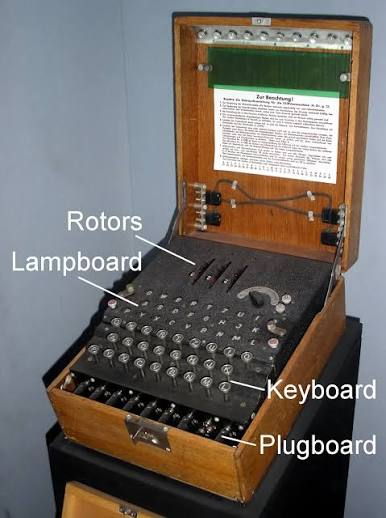
\includegraphics[height=7cm,keepaspectratio]
        {figs/Bayes_figs/Enigma.jpg}
    }

    \caption{A German Enigma machine.
    \href{https://en.wikipedia.org/wiki/Cryptanalysis_of_the_Enigma\#/media/File:EnigmaMachineLabeled.jpg}
    {Source: Wikipedia}.}

    \label{fig:enigma-machine}
\end{minipage}
\hspace{0.04\textwidth}
% --- Turing example ---
\begin{minipage}[t]{0.42\textwidth}
    \centering

    \href{https://arxiv.org/pdf/1505.04714}{
        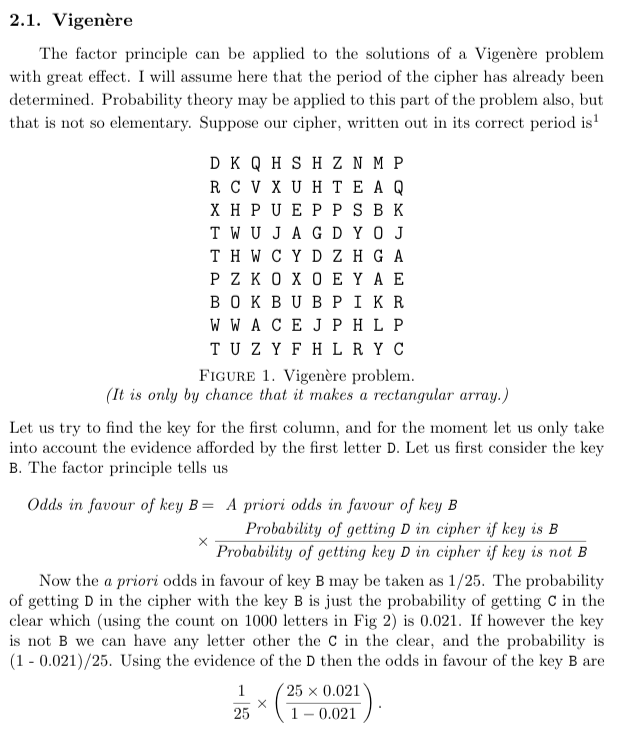
\includegraphics[height=7cm,keepaspectratio]
        {figs/Bayes_figs/Turing_Vigenere_example_bayesfactors.png}
    }

    \caption{Turing's Vigen\`ere cipher example in
    \textit{The Applications of Probability to Cryptography}.
    \href{https://arxiv.org/pdf/1505.04714}
    {Read the original text}.}

    \label{fig:turing-vigenere}
\end{minipage}

\end{figure}

For Naval Enigma, the difficulty could be formulated partly as a problem of \textbf{hypothesis testing}. Cryptanalysts compared pairs of intercepted messages by shifting one ciphertext relative to the other. Each possible alignment corresponded to a hypothesis about the difference between the rotor starting positions used to encrypt the two messages. If an alignment produced an unusually large number of matching letters or repeated patterns, this provided evidence that the messages had been encrypted at corresponding rotor positions, known as being \textit{in depth}. Such evidence could then help favour or eliminate possible rotor positions and rotor orders.

Let $H_1$ and $H_0$ denote two competing hypotheses about the cipher
configuration, and let $E$ denote the observed evidence---for example, the pattern of coincidences produced by a particular message alignment. In odds form, Bayes' theorem gives

\begin{equation}
\boxed{
\underbrace{
\frac{P(H_1\mid E)}{P(H_0\mid E)}
}_{\text{posterior odds}}
=
\underbrace{
\frac{P(H_1)}{P(H_0)}
}_{\text{prior odds}}
\;
\underbrace{
\frac{P(E\mid H_1)}{P(E\mid H_0)}
}_{\substack{\text{Bayes factor}\\\text{(likelihood ratio)}}}
}
\end{equation}


Thus the \textbf{prior odds} are multiplied by a \textbf{likelihood ratio} \textit{measuring how strongly the observed evidence favours one hypothesis over the other}.  Turing described this idea in his wartime manuscript \textit{The Applications of Probability to Cryptography}, calling it the \emph{factor principle (or Bayes' Theorem)} \cite{turing1941cryptography,zabell2012turing}.

% Thus the \textbf{prior odds} are multiplied by a likelihood ratio measuring
% how strongly the observed evidence favours one hypothesis over the other. In
% modern Bayesian terminology, this ratio is closely associated with the
% \textbf{\emph{Bayes factor}}. Turing described this idea in his wartime
% manuscript \textit{The Applications of Probability to Cryptography}, calling
% it the \emph{factor principle (or Bayes' Theorem)}
% \cite{turing1941cryptography,zabell2012turing}.

Because evidence from many message comparisons had to be combined,
multiplying likelihood ratios repeatedly was inconvenient. Turing therefore expressed the weight of evidence on a logarithmic scale using the \textbf{deciban},


% The difficulty was therefore partly one of \textbf{hypothesis testing}.
% Different rotor orders, positions or other proposed settings could be regarded
% as competing hypotheses. Evidence---including message patterns, probable
% plaintext, operator habits and repeated structures---could make some
% possibilities more plausible than others.

% Suppose $H_1$ and $H_0$ are two competing hypotheses about the cipher
% configuration and $E$ is newly observed evidence. In odds form, Bayes'
% theorem gives

% \begin{equation}
% \boxed{
% \frac{P(H_1\mid E)}{P(H_0\mid E)}
% =
% \frac{P(H_1)}{P(H_0)}
% \underbrace{\frac{P(E\mid H_1)}{P(E\mid H_0)}}_{\text{evidence}}
% }.
% \label{eq:turing-bayes-odds}
% \end{equation}

% Thus the \textbf{prior odds} are multiplied by a likelihood ratio measuring
% how strongly the new evidence favours one hypothesis over the other. In
% modern Bayesian terminology this evidence ratio is closely associated with
% the \textbf{\emph{Bayes factor}}. Turing described precisely this idea in his wartime
% manuscript \textit{The Applications of Probability to Cryptography}, calling
% it the \emph{factor principle (or Bayes' Theorem)}
% \cite{turing1941cryptography,zabell2012turing}.

% For Naval Enigma, cryptanalysts compared pairs of intercepted messages by shifting one ciphertext against the other. \textbf{Each possible shift represented a hypothesis} about the difference between the rotor starting positions used to encrypt the two messages. If a particular alignment produced an unusually large number of matching letters or repeated patterns, this provided statistical evidence that the messages had been encrypted at corresponding rotor positions, known as being in \textit{depth}. Evidence from several such comparisons could then be combined to favour or reject possible rotor orders. Turing expressed these likelihood comparisons logarithmically using the \textbf{deciban},

\begin{equation}
\boxed{
D
=
10\log_{10}
\left(
\frac{P(E\mid H_1)}{P(E\mid H_0)}
\right).
}
\end{equation}

On this scale, successive pieces of evidence could be \textbf{added} rather than multiplied. Ten decibans multiplied the odds by $10$, while one deciban changed them by a factor of $10^{0.1}\approx1.26$. These ideas formed part of Turing's statistical procedure known as \emph{Banburismus}, which helped cryptanalysts rank possibilities and reduce the amount of scarce Bombe machine time devoted to unlikely settings \cite{good1979turing,zabell2012turing}.

The importance of Turing's contribution was therefore not the invention of Bayesian hypothesis testing itself, which had earlier roots in the work of Wrinch, Haldane and Jeffreys, but its transformation into a practical method for \textbf{weighing accumulating evidence between competing hypotheses under severe computational constraints}. Good later helped bring these wartime
statistical ideas into the public literature  \cite{good1950,good1979turing}.

% bayes.tex, begins with \chapter{Bayes' Theorem}
% \include{mcmc}           % mcmc.tex, begins with \chapter{...}
% \include{filters}        % filters.tex, begins with \chapter{...}

\newpage


\bibliographystyle{plainnat}
\bibliography{references}
\end{document}